\documentclass[11pt]{article}

\usepackage[utf8]{inputenc}
\usepackage[ngerman]{babel}
\usepackage[T1]{fontenc}
\usepackage{amsmath}
\usepackage{siunitx} 
\usepackage{extarrows}
\sisetup{locale=DE, per-mode=symbol}

\usepackage{tikz}
\usepackage{tikz-cd}
\usepackage{import}

\usepackage{multicol}

\usepackage{graphics}
\usepackage{lipsum,multicol}

\usepackage{pgfplots}
\pgfplotsset{compat=1.12}

\usepackage{calrsfs}
\DeclareMathAlphabet{\pazocal}{OMS}{zplm}{m}{n}

\usepackage{setspace}

\usepackage{cancel}

\usepackage{listings}

\usepackage{subfig}
\usepackage[style=alphabetic, backend=biber]{biblatex}
% sorting=none, alldates=short, abbreviate=false, maxcitenames=2, maxbibnames=99, eprint=false, hyperref=auto,
\usepackage{pdfpages}
\usepackage{epstopdf}
\graphicspath{{images/}}

\usepackage[top=4cm, bottom=4cm, right=2cm, left=2cm]{geometry}

\title{Software Engineering: Wartung und Qualitätssicherung}



\newcommand{\dex}{\Delta x}
\newcommand{\pex}{\partial x}
\newcommand{\delt}{\Delta t}
\newcommand{\pet}{\partial t}
	
\begin{document}
	\maketitle
	\pagestyle{headings} %Kopf- und Fußzeile an
	
% 	\setcounter{tocdepth}{2} %Tiefe des Inhaltsverzeichnisses
% 	\tableofcontents %Inhaltsverzeichnis erstellen

		\section{Software-Entwicklung, Wartung und (Re)Engineering}
	Erstellte Software muss oft geändert werden, entweder aufgrund von geänderten Anforderungen oder neuen Anforderungen, welche eingebaut werden müssen.
	\subsection{Einleitung}
	\subsubsection{Geschichte}
	\begin{itemize}
		\item Softwarekrise 1968
		\item Nato \textbf{Working Conference on Software Engineering}
		\item Zuordnungen
		\begin{itemize}
			\item Praktische Informatik
			\item Theoretische Informatik
			\item Projektplanung
			\item Organisation
			\item Psychologie
			\item ...
		\end{itemize}
	\end{itemize}
	\subsubsection{''Software-Technik'' Definition}
	Software-Engineering(Software-Technik) ist nach \textbf{Entwicklung}, \textbf{Pflege} und \textbf{Einsatz}.
	\par 
	Eingesetzt werden:
	\begin{itemize}
		\item Wissenschaftliche Methoden
		\item Wirtschaftliche Prinzipien
		\item Geplante Vorgehensmodellen
		\item Werkzeuge
		\item Quantifizierbare Ziele
	\end{itemize}
	\subsubsection{50 Jahre nach Beginn der "Software-Krise"}
	\begin{itemize}
		\item 19\% aller Projekte sind gescheitert, früher 25\%
		\item 52\% aller Projekte sind dabei zu scheitern, früher 50\%
		\item 29\% aller betrachteten IT-Projekte sind erfolgreich, früher 25\%
	\end{itemize}
	Hauptgründe fürs Scheitern der Projekte:
	\par 
	Unklare Anforderungen und Abhängigkeiten sowie Problemen beim Änderungsmanagement.
	\subsection{Software-Qualität}
	Ziel der Software-Technik ist die effiziente Entwicklung messbar qualitativ hochwertiger Software.
	\par 
	\subsubsection{Qualitätsdefinition}
	Qualität ist der Grad, in dem ein System, eine Komponente oder ein Prozess die Kundenerwartungen und Kundenbedürfnisse erfüllt. 
	\subsubsection{Softwarequalität}
	Softwarequalität ist die Gesamtheit der Funktionalitäten und Merkmale eines Softwareprodukts, die sich auf dessen Eignung beziehen, festgelegte oder vorausgesetzte Erfordernisse zu erfüllen.
	\subsubsection{Qualitätsmerkmale}
	\begin{itemize}
		\item Funktionalität
	\end{itemize}
	\subsubsection{Nichtfunktionale Merkmale}
	\begin{itemize}
		\item Zuverlässigkeit (Reliability)
		\item Benutzbarkeit (Usability)
		\item Effizienz (Efficiency)
		\item Änderbarkeit (Maintainability)
		\item Übertragbarkeit (Portability)
	\end{itemize}
	\subsubsection{Prinzipien der Qualitätssicherung}
	\begin{itemize}
		\item \textbf{Qualitätszielbestimmung}: Auftraggeber und Auftragnehmer legen vor Beginn der Software-Entwicklung gemeinsames Qualitätsziel für Software-System mit nachprüfbaren Kriterienkatalog fest (als Bestandteil des abgeschlossenen Vertrags zur Software-Entwicklung)
		\item \textbf{Quantitative Qualitätssicherung}: Einsatz automatisch ermittelbaren Metriken zur Qualitätsbestimmung (objektivbare, ingenieursmäßige Vorgehensweise)
		\item \textbf{Konstruktive Qualitätssicherung}: Verwendung geeigneter Methoden, Sprachen und Werkzeuge (Vermeidung von Qualitätsproblemen)
		\item \textbf{Integrierte, frühzeitige, analytische Qualitätssicherung}: Systematische Prüfung aller erzeugter Dokumente (Aufdeckung von Qualitätsproblemen)
		\item \textbf{Unabhängige Qualitätssicherung}: Entwicklungsprodukte werden durch eigenständige Qualitätssicherungsabteilung überprüft und abgenommen (verhindert u.a. Verzicht auf Testen zugunsten Einhaltung des Entwicklungsplans)
	\end{itemize}
	\subsubsection{Konstruktives Qualitätssicherung zur Fehlervermeidung}: 
	\begin{itemize}
		\item Technische Maßnahmen
		\begin{itemize}
			\item Sprachen (UML, Java)
			\item Werkzeuge (UML-CASE-TOOL)
		\end{itemize}
		\item Organisatorische Maßnahmen
		\begin{itemize}
			\item Richtlinien (Gliederungsschema für Pflichtenheft, Programmierrichtlinien)
			\item Standards (für verwendete Sprachen, Dokumentformate, Management)
			\item Checklisten
		\end{itemize}
	\end{itemize}
	\subsubsection{Analytisches Qualitätsmanagement für Fehleridentifikation}
	\begin{itemize}
		\item \textbf{Analysierende Verfahren}: Der "Prüfling" (Programm, Modell, Dokumentation) wird von Menschen oder Werkzeugen auf Vorhandensein/Abwesenheit von Eigenschaften untersucht
		\begin{itemize}
			\item \textbf{Review}: Prüfung durch Menschen
			\item \textbf{Statische Analyse}: Werkzeuggestützte Ermittlung von "Anomalien"
			\item \textbf{Formale Verifikation}: Werkzeuggestützter Beweis von Eigenschaften
		\end{itemize}
		\item \textbf{Testende Vefahren}: Der "Prüfling" wird mit konkreten oder abstrakten Eingabewerten auf einem Rechner ausgeführt
		\begin{itemize}
			\item \textbf{Dynamischer Test}: "normale" Ausführung mit ganz konkreten Eingaben
			\item \textbf{Symbolischer Test}: Ausführung mit symbolischen Eingaben
		\end{itemize}
	\end{itemize}
	\subsection{Iterative Softwareentwicklung}
	Voraussetzung für den sinnvollen Einsatz von Notationen und Werkzeugen zur Software-Entwicklung ist ein:
	\begin{itemize}
		\item \textbf{Vorgehensmodell}, das den Gesamtprozess der Software-Erstellung und pflege in einzelne Schritte aufteilt
		\item Zusätzlich müssen Verantwortlichkeiten der beteiligten Personen in Form von \textbf{Rollen} im Software-Entwicklungsprozess klar geregelt sein.
	\end{itemize}
	\subsubsection{Übersicht der Phasen des Wasserfallmodells}
	\begin{tikzpicture}[
		base/.style = {rectangle, rounded corners, draw=black,
		text centered, font=\sffamily},
		minimum width=4cm,
		blueStyle/.style = {base, fill=blue!30},]
		\node (machbarkeitsstudie) [blueStyle] {Machbarkeitsstudie};
		\node (anforderungsanalyse) [blueStyle, below of=machbarkeitsstudie, yshift=-0.5cm, xshift=1.2cm] {Anforderungsanalyse};
		\node (systementwurf) [blueStyle, below of=anforderungsanalyse, yshift=-0.5cm, xshift=1.2cm] {Systementwurf};
		\node (codieren) [blueStyle, below of=systementwurf, yshift=-0.5cm, xshift=1.2cm] {Codieren und Modultest};
		\node (integration) [blueStyle, below of=codieren, yshift=-0.5cm, xshift=1.2cm] {Integrations und Systemtest};
		\node (auslieferung) [blueStyle, below of=integration, yshift=-0.5cm, xshift=1.2cm] {Auslieferung und Installation};
		\node (wartung) [blueStyle, below of=auslieferung, yshift=-0.5cm, xshift=1.2cm] {Wartung};
		\draw[->] (machbarkeitsstudie) -- (anforderungsanalyse);
		\draw[->] (anforderungsanalyse) -- (systementwurf);
		\draw[->] (systementwurf) -- (codieren);
		\draw[->] (codieren) -- (integration);
		\draw[->] (integration) -- (auslieferung);
		\draw[->] (auslieferung) -- (wartung);
	\end{tikzpicture}
	\subsubsection{Machbarkeitsstudie (feasability study)}
	Die Machbarkeitsstudie schätzt Kosten und Ertrag der geplanten Software-Entwicklung ab. Dazu grobe Analyse des Problems mit Lösungsvorschlägen.
	\begin{itemize}
		\item \textbf{Aufgaben}
		\begin{itemize}
			\item Problem informell und abstrahiert beschreiben
			\item Verschiedene Lösungsansätze erarbeiten
			\item Kostenschätzung durchführen
			\item Angebotserstellung
		\end{itemize}
		\item \textbf{Ergebnisse}
		\begin{itemize}
			\item Lastenheft
			\item Projektkalkulation
			\item Projektplan
			\item Angebot an Auftraggeber
		\end{itemize}
	\end{itemize}
	\subsubsection{Anforderungsanalyse (requirements engineering)}
	In der Anforderungsanalyse wird exakt festgelegt, was die Software leisten soll, aber nicht wie diese Leistungsmerkmale erreicht werden.
	\begin{itemize}
		\item \textbf{Aufgaben}
		\begin{itemize}
			\item genaue Festlegung der Systemeigenschaften wie Funktionalität, Leistung, Benutzungsschnittstelle, Portierbarkeit, … im Pflichtenheft
			\item Bestimmen von Testfällen
			\item Festlegung erforderlicher Dokumentationsdokumente
		\end{itemize}
		\item \textbf{Ergebnisse}
		\begin{itemize}
			\item Pflichtenheft = Anforderungsanalysedokument 
			\item Akzeptanztestplan
			\item Benutzungshandbuch (1-te Version)
		\end{itemize}
	\end{itemize}
	\subsubsection{Systementwurf (system design/programming-in-the-large)}
	Im Systementwurf wird exakt festgelegt, wie die Funktionen der Software zu realisieren sind. Es wird der Bauplan der Software, die Software-Architektur, entwickelt.
	\begin{itemize}
		\item \textbf{Aufgaben}
		\begin{itemize}
			\item Programmieren-im-Großen = Entwicklung eines Bauplans
			\item Grobentwurf, der System in Teilsysteme/Module zerlegt
			\item Auswahl bereits existierender Software-Bibliotheken, Rahmenwerke, …
			\item Feinentwurf, der Modulschnittstellen und Algorithmen vorgibt
		\end{itemize}
		\item \textbf{Ergebnisse}
		\begin{itemize}
			\item Entwurfsdokument mit Software-Bauplan
			\item detaillierte(re) Testpläne
		\end{itemize}
	\end{itemize}
	\subsubsection{Codieren und Modultest (programming-in-the-small)}
	Die eigentliche Implementierungs- und Testphase, in der einzelne Module (in einer bestimmten Reihenfolge) realisiert und validiert werden.
	\begin{itemize}
		\item \textbf{Aufgaben}
		\begin{itemize}
			\item Programmieren-im-Kleinen = Implementierung einzelner Module
			\item Einhaltung von Programmierrichtlinien
			\item Code-Inspektionen kritischer Modulteile (Walkthroughs)
			\item Test der erstellten Module
		\end{itemize}
		\item \textbf{Ergebnisse}
		\begin{itemize}
			\item Menge realisierter Module
			\item Implementierungsberichte (Abweichungen vom Entwurf, Zeitplan, … )
			\item Technische Dokumentation einzelner Module
			\item Testprotokolle
		\end{itemize}
	\end{itemize}
	\subsubsection{Integrations- und Systemtest}
	Die einzelnen Module werden schrittweise zum Gesamtsystem zusammengebaut. Diese Phase kann mit der vorigen Phase verschmolzen werden, falls der Test isolierter Module nicht praktikabel ist.
	\begin{itemize}
		\item \textbf{Aufgaben}
		\begin{itemize}
			\item Systemintegration = Zusammenbau der Module
			\item Gesamtsystemtest in Entwicklungsorganisation durch Kunden (alpha-Test)
			\item Fertigstellung der Dokumentation
		\end{itemize}
		\item \textbf{Ergebnisse}
		\begin{itemize}
			\item Fertiges System
			\item Benutzerhandbuch
			\item Technische Dokumentation
			\item Testprotokolle
		\end{itemize}
	\end{itemize}
	\subsubsection{Auslieferung und Installation}
	Die Auslieferung (Installation) und Inbetriebnahme der Software beim Kunden findet häufig in zwei Phasen statt.
	\begin{itemize}
		\item \textbf{Aufgaben}
		\begin{itemize}
			\item Auslieferung an ausgewählte (Pilot-)Benutzer (Beta-Test)
			\item Auslieferung an alle Benutzer
			\item Schulung der Benutzer
		\end{itemize}
		\item \textbf{Ergebnisse}
		\begin{itemize}
			\item Fertiges System
			\item Akzeptanztestdokument
		\end{itemize}
	\end{itemize}
	\subsubsection{Wartung (Maintenance)}
	Nach der ersten Auslieferung der Software an die Kunden beginnt das Elend der Software-Wartung, das ca. 60\% der gesamten Software-Kosten ausmacht.
	\begin{itemize}
		\item \textbf{Aufgaben}
		\begin{itemize}
			\item ca. 20\% Fehler beheben (corrective maintenance)
			\item ca. 20\% Anpassungen durchführen (adaptive maintenance)
			\item ca. 50\% Verbesserungen vornehmen (perfective maintenance)
		\end{itemize}
		\item \textbf{Ergebnisse}
		\begin{itemize}
			\item Software-Problemberichte (bug reports)
			\item Software-Änderungsvorschläge
			\item Neue Software-Versionen
		\end{itemize}
	\end{itemize}
	\subsubsection{Probleme mit dem Wasserfallmodell}
	\begin{itemize}
		\item zu Projektbeginn sind nur ungenaue Kosten- und Ressourcenschätzungen möglich
		\item ein Pflichtenheft kann nie den Umgang mit dem fertigen System ersetzen, das erste sehr spät entsteht (Risikomaximierung)
		\item es gibt Fälle, in denen zu Projektbeginn kein vollständiges Pflichtenheft erstellt werden kann (weil Anforderungen nicht klar)
		\item Anforderungen werden früh eingefroren, notwendiger Wandel (aufgrund organisatorischer, politischer, technischer, … Änderungen) nicht eingeplant
		\item strikte Phaseneinteilung ist unrealistisch (Rückgriffe sind notwendig)
		\item Wartung mit ca. 60\% des Gesamtaufwandes ist eine Phase
	\end{itemize}
	\begin{figure}[h]
		\centering
		\caption{Andere Darstellung der Aufwandsverteilung}
		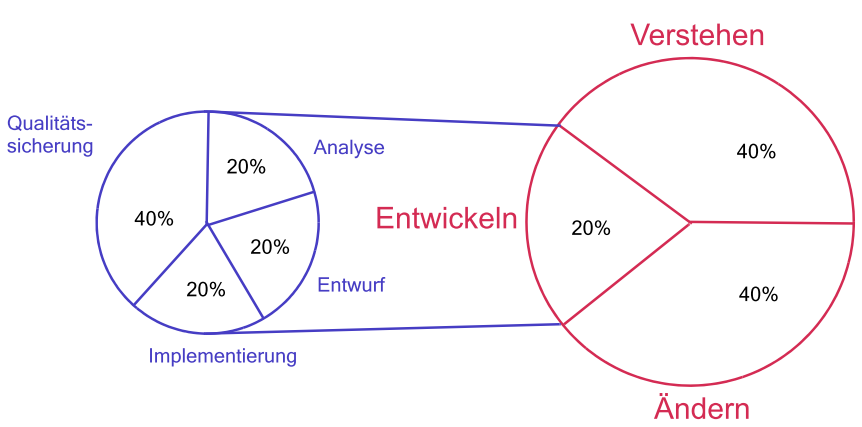
\includegraphics[width=0.65\textwidth]{taskDistribution}
	\end{figure}
	\subsubsection{Typische Probleme in der Wartungsphase}
	\begin{itemize}
		\item Einsatz wenig erfahrenen Personals (nicht Entwicklungspersonal)
		\item Fehlerbehebung führt neue Fehler ein
		\item Stetige Verschlechterung der Programmstruktur
		\item Zusammenhang zwischen Programm und Dokumentation geht verloren
		\item Zur Entwicklung eingesetzte Werkzeuge (CASE-Tools, Compiler, … ) sterben aus
		\item Benötigte Hardware steht nicht mehr zur Verfügung
		\item Resourcenkonflikte zwischen Fehlerbehebung und Anpassung/Erweiterung
		\item Völlig neue Ansprüche an Funktionalität und Benutzeroberfläche
	\end{itemize}
	\subsection{Forward-, Reverse- und Reengineering}
	\subsubsection{Software Evolution}
	\begin{itemize}
		\item Wünsche
		\begin{itemize}
			\item Wartung ändert Software kontrolliert ohne Design zu zerstören
			\item Konsistenz aller Dokumente bleibt erhalten
		\end{itemize}
		\item Wirklichkeit
		\begin{itemize}
			\item Ursprüngliche Systemstruktur wird ignoriert
			\item Dokumentation wird unvollständig oder unbrauchbar
			\item Mitarbeiter verlassen Projekt
		\end{itemize}
	\end{itemize}
	\subsubsection{Forward Engineering}
	Beim Forward Engineering ist das fertige Softwaresystem das Ergebnis des Entwicklungsprozesses. Ausgehend von Anforderungsanalyse (Machbarkeitsstudie) wird ein neues Softwaresystem entwickelt.
	\subsubsection{Reverse Engineering}
	Beim Reverse Engineering ist das vorhandene Software-System der Ausgangspunkt der Analyse. Ausgehend von existierender Implementierung wird meist „nur“ das Design rekonstruiert und dokumentiert. Es wird (noch) nicht das betrachtete System modifiziert.
	\subsubsection{Reengineering}
	Reengineering befaßt sich mit der Sanierung eines vorhandenen Software-Systems bzw. seiner Neuimplementierung. Dabei werden die Ergebnisse des Reverse Engineerings als Ausgangspunkt genommen
	\begin{figure}[h]
		\centering
		\caption{Round Trip Engineering}
		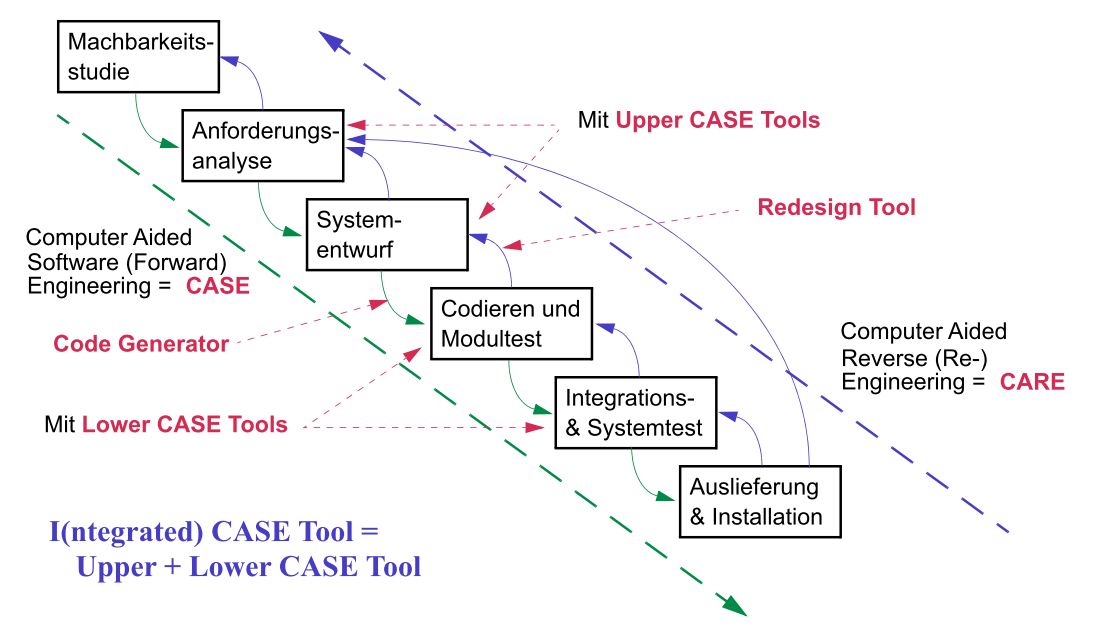
\includegraphics[width=0.85\textwidth]{roundTripEngineering}
	\end{figure}
	\begin{figure}[h]
		\centering
		\caption{Einfaches Software-Lebenszyklus-Prozessmodell für die Wartung}
		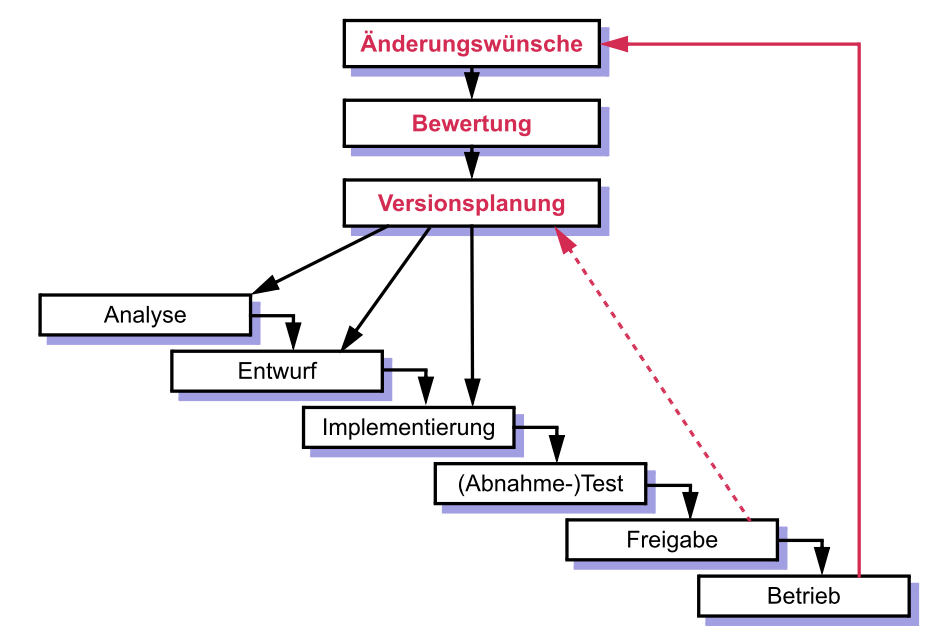
\includegraphics[width=0.85\textwidth]{softwareCycle-1}
	\end{figure}
	\subsubsection{Das V-Modell}
	\begin{itemize}
		\item \textbf{Systemanforderungsanalyse}: Gesamtsystem einschließlich aller Nicht-DV-Komponenten wird beschrieben (fachliche Anforderungen und Risikoanalyse)
		\item \textbf{Systementwurf}: System wird in technische Komponenten (Subsysteme) zerlegt, also die Grobarchitektur des Systems definiert
		\item \textbf{Softwareanforderungsanalyse}: Technischen Anforderungen an die bereits identifizierten Komponenten werden definiert
		\item \textbf{Softwaregrobentwurf}: Softwarearchitektur wird bis auf Modulebene festgelegt
		\item \textbf{Softwarefeinentwurf}: Details einzelner Module werden festgelegt
		\item \textbf{Softwareimplementierung}: Wie beim Wasserfallmodell (inklusive Modultest) 
		\item \textbf{Software-/Systemintegration:}: Schrittweise Integration und Test der verschiedenen Systemanteile
		\item \textbf{Überleitung in die Nutzung:}: Entspricht Auslieferung bei Wasserfallmodell
	\end{itemize}
	\begin{figure}[h]
		\centering
		\caption{Das V-Modell}
		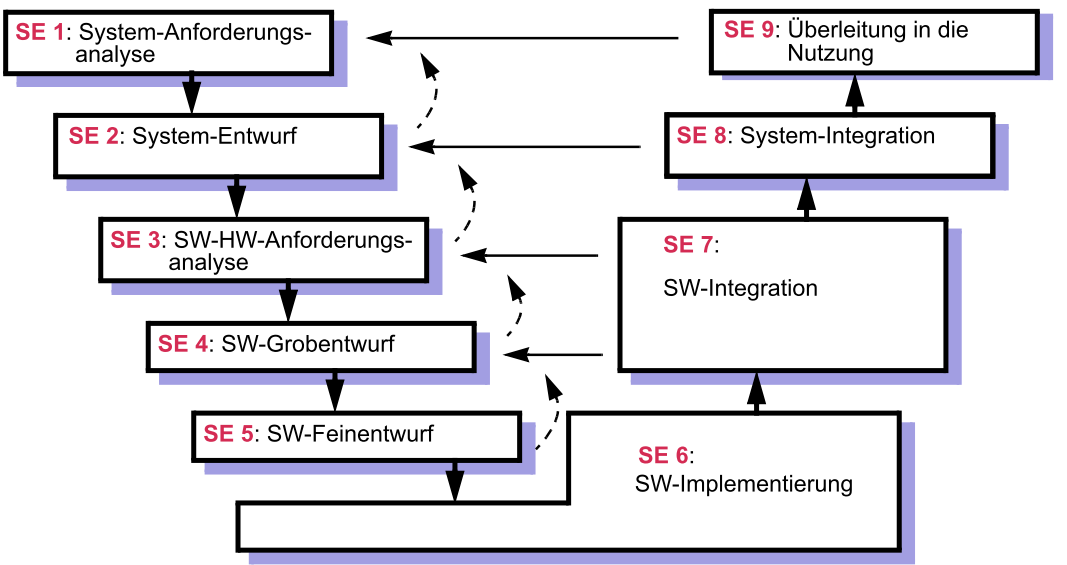
\includegraphics[width=0.85\textwidth]{v-model}
	\end{figure}

	\section{Konfigurationsmanagement}
Beim Konfigurationsmanagement handelt es sich um die Entwicklung und Anwendung von Standards und Verfahren zur Verwaltung eines sich weiterentwickelnden Systemprodukts.
\subsection{Einleitung}
\subsubsection{Fragestellungen}
\begin{itemize}
	\item Das System lief gestern noch; was hat sich seitdem geändert?
	\item Wer hat diese (fehlerhafte?) Änderung wann und warum durchgeführt?
	\item Wer ist von meinen Änderungen an dieser Datei betroffen?
	\item Auf welche Version des Systems bezieht sich die Fehlermeldung?
	\item Wie erzeuge ich Version x.y aus dem Jahre 1999 wieder?
	\item Welche Fehlermeldungen sind in dieser Version bereits bearbeitet?
	\item Welche Erweiterungswünsche liegen für das nächste Release vor?
	\item  Die Platte ist hinüber; was für einen Status haben die Backups?
\end{itemize}
\subsubsection{Definitionen}
\paragraph{Definition von Software-KM nach IEEE-Standard 828-1988}
SCM (Software Configuration Management) constitutes \textbf{good engineering practice } for all software projects, whether phased development, rapid prototyping, or ongoing  maintenance. It enhances the reliability and quality of software by:
\begin{itemize}
	\item Providing structure for \textbf{identifying and controlling} documentation, code, interfaces, and databases to support all life cycle phases
	\item Supporting a chosen \textbf{development/maintenance methodology} that fits the requirements, standards, policies, organization, and management philosophy
	\item Producing \textbf{management and product information} concerning the status of baselines, change control, tests, releases, audits etc.
\end{itemize}
Diese Definition ist jedoch nicht konkret und unabhängig vom Begriff ''Software''
\paragraph{Definition nach DIN EN ISO 10007}
KM (Konfigurationsmanagement) ist eine Managementdisziplin, die über die gesamte Entwicklungszeit eines Erzeugnisses angewandt wird, um Transparenz und Überwachung seiner funktionellen und physischen Merkmale sicherzustellen.
\\
Der KM-Prozess umfasst die folgenden integrierten Tätigkeiten:
\begin{itemize}
	\item \textbf{Konfigurationsidentifizierung}: Definition und Dokumentation der Bestandteile eines Erzeugnisses, Einrichten von Bezugskonfigurationen, ...
	\item \textbf{Konfigurationsüberwachung}: Dokumentation und Begründung von Änderungen, Genehmigung oder Ablehnung von Änderungen, Planung von Freigaben, ...
	\item \textbf{Konfigurationsbuchführung}: Rückverfolgung aller Änderungen bis zur letzten Bezugskonfiguration, ...
	\item \textbf{Konfigurationsauditierung}: Qualitätssicherungsmaßnahmen für Freigabe einer Konfiguration eines Erzeugnisses
	\item \textbf{KM-Planung}: Festlegung der Grundsätze und Verfahren zum KM in Form eines KM-Plans
\end{itemize}
\paragraph{Werkzeugorientierte Sicht auf KM-Aktivitäten}
\begin{enumerate}
	\item \textbf{KM-Planung}: Beschreibung der Standards, Verfahren und Werkzeuge, die für KM benutzt werden; wer darf/muss wann was machen
	\item \textbf{Versionsmanagement}: Verwaltung der Entwicklungsgeschichte eines Produkts; also wer hat wann, wo, was und warum geändert
	\item \textbf{Variantenmanagement}: Verwaltung parallel existierender Ausprägungen eines Produkts für verschiedene Anforderungen, Länder, Plattformen
	\item \textbf{Releasemanagement}: Verwaltung und Planung von Auslieferungsständen; wann wird eine neue Produktversion mit welchen Features auf den Markt geworfen  
	\item \textbf{Buildmanagement}: Erzeugung des auszulieferenden Produkts; wann muss welche Datei mit welchem Werkzeug generiert, übersetzt, ... werden
	\item \textbf{Änderungsmanagement}: Verwaltung von Änderungsanforderungen; also Bearbeitung von Fehlermeldungen und Änderungswünschen (Feature Requests) sowie Zuordnung zu Auslieferungsständen
\end{enumerate}
\begin{figure}[h]
	\caption{Integration des Konfigurationsmanagements im V-Modell}
	\centering
	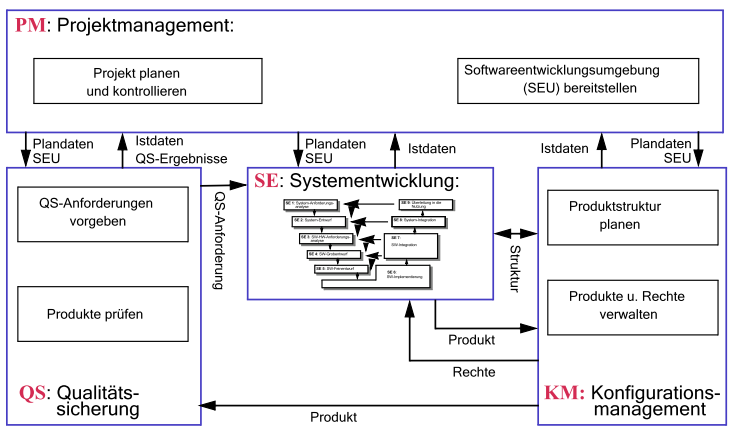
\includegraphics[width=0.85\textwidth]{2_1_1}
\end{figure}
\begin{figure}[h]
	\caption{Grafische Übersicht über Aufgaben- und Rollenverteilung}
	\centering
	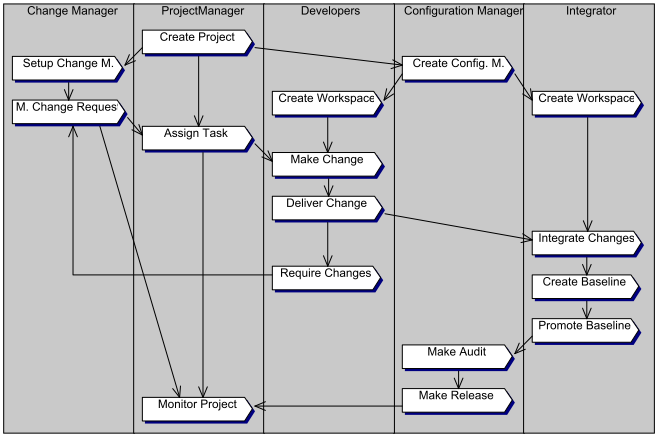
\includegraphics[width=0.85\textwidth]{2_1_2}
\end{figure}
\paragraph{Workspaces für das Konfigurationsmanagement}
\begin{figure}[h]
	\caption{Workspaces für das Konfigurationsmanagement}
	\centering
	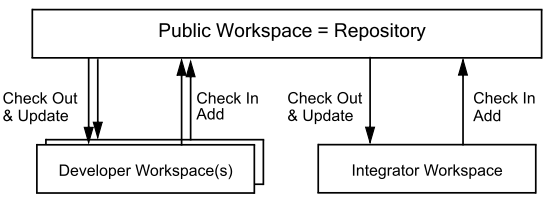
\includegraphics[width=0.6\textwidth]{2_1_3}
\end{figure}
\begin{itemize}
	\item alle Dokumente (Objekte, Komponenten) zu einem bestimmten Projekt werden in	einem gemeinsamen Repository (\textbf{public workspace}) aufgehoben
	\item im Repository werden nicht nur aktuelle Versionen, sondern auch alle \textbf{früheren Versionen} aller Dokumenten gehalten
	\item beteiligte Entwickler bearbeiten ihre eigenen Versionen dieser Dokumente in 
	ihrem privaten Arbeitsbereich (private workspace, \textbf{developer workspace}) 
	\item es gibt genau einen Integrationsarbeitsbereich (\textbf{integrations workspace}) für die Systemintegration
\end{itemize}
\paragraph{Aktivitäten bei der Arbeit mit Workspaces}
\begin{itemize}
	\item Personen holen sich Versionen neuer Dokumente, die von anderen Personen erstellt wurden(\textbf{checkout}), ih ihren privaten Arbeitsbereich
	\item Personen passen ihre Privatversionen ggf. von Zeit zu Zeit an neue Versionen im öffentlichen Repository an (\textbf{update}).
	\item Sie fügen (hoffentlich) nur konsistente Dokumente als neue Versionen in das allgemeine Repository ein (\textbf{checkin = commit}).
	\item Ab und an werden neue Dokumente dem Repository hinzugefügt (\textbf{add}). 
	\item Jede Person kann alte/neue Versionen frei wählen.
\end{itemize}
\paragraph{Probleme}
\begin{itemize}
	\item Wie wird Konsistenz von Gruppen abhängiger Dokumente sichergestellt?
	\item Was passiert bei gleichzeitigen Änderungswünschen für ein Dokument?
	\item Wie realisiert man die Repository-Operationen effizient?
	\item Wie unterstützt man ''Offline''-Arbeit (ohne Zugriff auf Repository)?
\end{itemize}
\paragraph{Weitere Begriffe des Konfigurationsmanagements}
\begin{itemize}
	\item \textbf{Dokument} = Gegenstand, der der Konfigurationsverwaltung unterworfen wird (eine einzelne Datei oder ein ganzer Dateibaum oder ... )
	\item \textbf{(Versions-)Objekt} = Zustand einer Dokument zu einem bestimmten Zeitpunkt in einer bestimmten Ausprägung
	\item \textbf{Varianten} = parallel zueinander (gleichzeitig) existierende Ausprägungen eines Dokuments, die unterschiedliche Anforderungen erfüllen
	\item \textbf{Revisionen} = zeitlich aufeinander folgende Zustände eines Dokuments
	\item  \textbf{Konfiguration} = komplexes Versionsobjekt, eine bestimmte Ausprägung eines Programmsystems (oft hierarchisch strukturierte Menge von Dokumenten)
	\item \textbf{Baseline} = eine Konfiguration, die zu einem Meilenstein (Ende einer Entwicklungsphase) gehört und evaluiert (getestet) wird
	\item \textbf{Release} = eine stabile Baseline, die ausgeliefert wird (intern an Entwickler oder extern an bestimmte Kunden oder ... )
\end{itemize}
\subsection{Versionsmanagement}
Bekannteste ''open source''-Produkte (in zeitlicher Reihenfolge) sind:
\begin{itemize}
	\item Source Code Control System \textbf{SCCS} von AT\&T (Bell Labs):
	\begin{itemize}
		\item effiziente Speicherung von Textdateiversionen als ''Patches''
	\end{itemize}
	\item Revision Control System \textbf{RCS} von Berkley/Purdue University
	\begin{itemize}
		\item schnellerer Zugriff auf Textdateiversionen
	\end{itemize}
	\item Concurrent Version (Control) System \textbf{CVS} (zunächst Skripte für RCS)
	\begin{itemize}
		\item Verwaltung von Dateibäumen
		\item parallele Bearbeitung von Textdateiversionen
	\end{itemize}
	\item Subversion \textbf{SVN} - CVS-Nachfolger von CollabNet initiiert (http://www.collab.net)
	\begin{itemize}
		\item Versionierung von Dateibäumen
	\end{itemize}
	\item \textbf{Git}, Mercurial, ... als verteilte Versionsmanagementsysteme
	\begin{itemize}
		\item jeder Entwickler hat eigene/lokale Versionsverwaltung
	\end{itemize}
\end{itemize}
\subsubsection{Source Code Control System SCCS von AT\&T (Bell Labs)}
Je Dokument (Quelltextdatei) gibt es eine eigene \textbf{History-Datei}, die alle Revisionen als eine Liste jeweils geänderter (Text-)Blöcke speichert:
\begin{itemize}
	\item jeder Block ist ein \textbf{Delta}, das Änderungen zwischen Vorgängerrevision und aktueller Revision beschreibt
	\item jedes Delta hat \textbf{SCCS-Identifikationsnummer} der zugehörigen Revision: <ReleaseNo>.<LevelNo>.<BranchNo>.<SequenceNo>
\end{itemize}
\paragraph{Revisionsbäume von SCSS}
\begin{itemize}
	\item Release 1.1 \ Neuentwicklung
	\item Release 1.1 \ Wartung
	\item Release 1.2 \ Weiterentwicklung
	\item Release 2 \ Weiterentwicklung
\end{itemize}
\paragraph{Erläuterungen zu ''diff'' und ''patch''}
\begin{itemize}
	\item ''\textbf{diff}''-Werkzeug bestimmt Unterschiede zwischen (Text-)Dateien = \textbf{Deltas}
	\item ein Delta(diff) zwischen zwei Textdateien besteht aus einer Folge von ''Hunks'', die jeweils Änderungen eines Zeilenbereichs beschreiben:
	\begin{itemize}
		\item Änderungen von Zeilen: werden mit ''\textbf{!}'' markiert
		\item Hinzufügen von Zeilen: werden mit ''\textbf{+}'' markiert
		\item Löschen von Zeilen: werden mit ''\textbf{-}'' markiert
	\end{itemize}
	\item reale Deltas enthalten unveränderte \textbf{Kontextzeilen} zur besseren Identifikation von Änderungsstellen
	\item ein \textbf{Vorwärtsdelta} zwischen zwei Dateien d1 und d2 kann als ''\textbf{patch}'' zur Erzeugung von Datei d2 auf Datei d1 angewendet werden
	\item inverses \textbf{Rückwärtsdelta} zwischen zwei Dateien d1 und d2 kann als ''patch'' zur Wiederherstellung von Datei d1 auf Datei d2 angewendet werden
	\item SCCS-Deltas sind in einer Datei gespeichert, deshalb weder Vorwärts- noch Rückwärts- sondern \textbf{Inline-Deltas}
\end{itemize}
\paragraph{Genauere Instruktionen zur Erzeugung von Deltas}
Jedes ''diff''-Werkzeug hat seine eigenen Heuristiken, wie es möglichst kleine und/oder lesbare Deltas/Patches erzeugt, die die Unterschiede zweier Dateien darstellen. Ein möglicher (und in den Übungen verwendeter) Satz von Regeln zur Erzeugung von Deltas sieht wie folgt aus:
\begin{enumerate}
	\item Die Anzahl der geänderten, gelöschten und neu erzeugten Zeilen aller Hunks eines \textbf{Deltas} zweier Dateien wird möglichst klein gehalten.
	\item Jeder Hunk beginnt mit genau einer unveränderten \textbf{Kontextzeile} und enthält sonst nur geänderte, gelöschte oder neu eingefügte Zeilen (Ausnahme: Dateianfang).
	\item Aufeinander folgende Hunks sind also durch jeweils \textbf{mindestens eine unveränderte Zeile} getrennt.
	\item Optional: Anstelle von Löschen und Neuerzeugen einer Zeile i verwendet man die 
	\textbf{Änderungsmarkierung ''!''}
\end{enumerate}
\paragraph{Durch diese Regeln nicht gelöstes Problem}
Wie erkenne ich, ob eine Änderung in Zeile i durch Einfügen einer neuen Zeile oder durch Ändern einer alten Zeile zustande gekommen ist?
\paragraph{Create- und Apply-Patch in Eclipse}
Die ''Create Patch''- und ''Apply Patch''-Funktionen in Eclipse benutzen genau das gerade eingeführte ''Unified Diff''-Format. Dabei werden bei der Erzeugung von Hunks wohl folgende Heuristiken/Regeln verwendet:
\begin{itemize}
	\item ein Hunk scheint in der Regel mit drei unveränderten Kontextzeilen zu beginnen (inklusive Leerzeilen).
	\item zwei Blöcke geänderter Zeilen müssen durch mindestens sieben unveränderte Zeilen getrennt sein, damit dafür getrennte Hunks erzeugt werden
\end{itemize}
Bei der Anwendung von Patches werden folgende Heuristiken/Regeln verwendet:
\begin{itemize}
	\item werden der Kontext oder die zu löschenden Zeilen eines Patches so nicht gefunden, dann endet die Patch-Anwendung mit einer Fehlermeldung
	\item befindet sich die zu patchende Stelle eines Textes nicht mehr an der angegebenen Stelle (Zeile), so wird trotzdem der Patch angewendet
	\item gibt es mehrere (identische) Stellen in einem Text, auf die ein Patch angewendet werden kann, so wird die Stelle verändert, die am nächsten zur alten Position ist
\end{itemize}
\paragraph{Eigenschaften von SCSS}
\begin{itemize}
	\item für beliebinge (Text-)Dateien verwendbar (und nur für solche
	\item Schreibsperren auf ''ausgecheckten'' Revisionen
	\item Revisionsbäume mit manuellem Konsistenthalten von Entwicklungszweigen
	\item Rekonstruktionszeit von Revisionen steigt linear mit der Anzahl der Revisionen (Durchlauf durch Blockliste)
	\item Revisionsidentifikation nur durch Nummer und Datum
\end{itemize}
\paragraph{Offene Probleme}
\begin{itemize}
	\item Kein Konfigurationsbegriff und kein Variantenbegriff
	\item Keine Unterstützung zur Verwaltung von Konsistenzbeziehungen zwischen verschiedenen Objekten
\end{itemize}
\paragraph{Probleme mit Schreibsperren}
SCCS realisiert ein sogenanntes ''pessimistisches'' Sperrkonzept. Gleichzeitige Bearbeitung einer Datei durch mehrere Personen wird verhindert:
\begin{itemize}
	\item ein Checkout zum Schreiben (\textbf{single write access})
	\item mehrere Checkouts zum Lesen (\textbf{multiple read access})
\end{itemize}
In der Praxis kommt es aber öfter vor, dass mehrere Entwickler dieselbe Datei zeitgleich verändern müssen (oder Person mit Schreibrecht ''commit'' vergisst...)
\paragraph{Unbefriedigende Lösungen}
\begin{itemize}
	\item Entwickler mit Schreibrecht macht ''commit'' unfertiger Datei, Entwickler mit dringendstem Änderungswunsch macht ''checkout'' mit Schreibrecht
	\begin{itemize}
		\item inkonsistente Zustände in Repository, nur einer darf ''Arbeiten''
	\end{itemize}
	\item weitere Entwickler mir Schreibwunsch ''stehlen'' Datei, machen also ''checkout'' mit Leserecht und modifizieren Datei trotzdem
	\begin{itemize}
		\item Problem: Verschmelzen der verschiedenen Änderungen
	\end{itemize}
\end{itemize}
\subsubsection{Revision Control System RCS von Berkley/Purdue University}Je Dokument (immer Textdatei) gibt es eine eigene History-Datei, die eine neueste Revision vollständig und andere Revisionen als \textbf{Deltas} speichert:
\begin{itemize}
	\item optionale \textbf{Schreibsperren} (verhindern ggf. paralleles Ändern)
	\item \textbf{Revisionsbäume} mit besserem Zugriff auf Revisionen:
	\begin{itemize}
		\item schneller Zugriff auf neueste Revision auf Hauptzweig
		\item langsamer Zugriff auf ältere Revisionen auf Hauptzweig  (mit \textbf{Rückwärtsdeltas})
		\item langsamer Zugriff auf Revisionen auf Nebenzweigen (mit \textbf{Vorwärtsdeltas}).
	\end{itemize}
	\item Versionsidentifikation auch durch frei wählbare Bezeichner
\end{itemize}
\paragraph{Offene Probleme}
Kein Konfigurationsbegriff und kein Variantenbegriff
\begin{figure}[h]
	\caption{Deltaspeicherung von Revisionen als gerichtete Graphen}
	\centering
	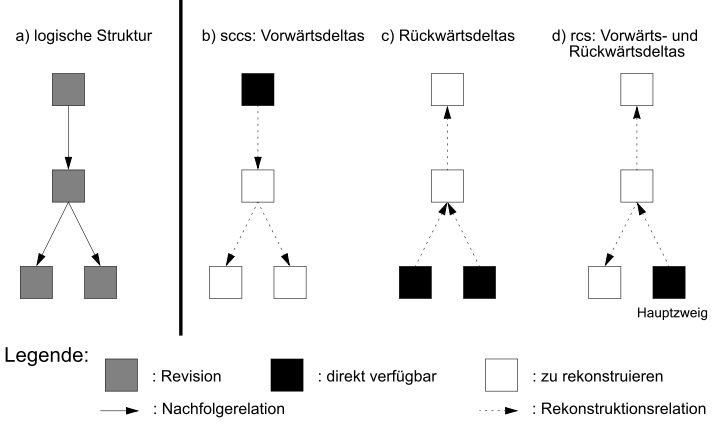
\includegraphics[width=0.85\textwidth]{2_2_1}
\end{figure}
\subsubsection{Concurrent Version (Management) System CVS}
\subsection{Releasemanagement}
\subsection{Buildmanagement}
\subsection{Änderungsmanagement}
\subsection{Zusammenfassung}




	\section{Statische Programmanalyse \& Metriken}
Statische Codeanalyse verlangt ein stures, monotones Anwenden von relativ ein-
fachen Regeln auf oft umfangreichen Code. Diese Aufgabe erfordert keinerlei Kreativität aber eine sehr große Übersicht und Kontrolle. ... Statische Codeanalyse ist daher prädestiniert zur Automatisierung durch Werkzeuge. Ich empfehle Ihnen, diese Techniken entweder werkzeuggestützt oder gar nicht einzusetzen.

\subsection{Einleitung}
\begin{itemize}
	\item Oft (fast immer) finden sich \textbf{80\% aller Probleme} mit einem Softwaresystem in 20\% des entwickelten Codes. 
	\item Die statische Programmanalyse versucht meist werkzeuggestützt frühzeitig die \textbf{problematischen 20\%} eines Softwaresystems zu finden.
	\item Statische Analyseverfahren identifizieren Programmteile von \textbf{fragwürdiger Qualität} und liefern damit Hinweise auf potentielle Fehlerstellen.
	\item Statische Analyseverfahren \textbf{versuchen} die Qualität von Software zu \textbf{messen}, können deshalb zur Festlegung von Qualitätsmaßstäben eingesetzt werden.
	\item Die statische Programmanalyse setzt \textbf{keine vollständig ausführbaren} Programme voraus.
	\item Die statische Programmanalyse kann also \textbf{frühzeitig} bei der Neuentwicklung und kontinuierlich bei der Wartung eines Softwaresystems eingesetzt werden.
\end{itemize}

\paragraph{Analytisches Qualitätsmanagement zur Fehleridentifikation:}
\begin{itemize}
	\item \textbf{analysierende Verfahren:} \\
	der ''Prüfling'' (Programm, Modell, Dokumentation) wird von Menschen oder Werkzeugen auf Vorhandensein/Abwesenheit von Eigenschaften untersucht
	\begin{itemize}
		\item \textbf{Review} (Inspektion, Walkthrough): Prüfung durch (Gruppe v.) Menschen
		\item \textbf{statische Analyse}: werkzeuggestützte Ermittlung von ''Anomalien''
		\item \textbf{(formale) Verifikation}: werkzeuggestützter Beweis von Eigenschaften 
	\end{itemize}
	\item \textbf{testende Verfahren:} \\
	der ''Prüfling'' wird mit konkreten oder abstrakten Eingabewerten auf einem Rechner ausgeführt
	\begin{itemize}
		\item \textbf{dynamischer Test}: ''normale'' Ausführung mit ganz konkreten Eingaben
		\item \textbf{[symbolischer Test}: Ausführung mit symbolischen Eingaben (die oft unendliche Mengen möglicher konkreter Eingaben repräsentieren)]
	\end{itemize}
\end{itemize}

\paragraph{Arten der Programmanalyse}
\begin{itemize}
	\item \textbf{Visualisierung von Programmstrukturen}: unästhetisches Layout liefert Hinweise auf sanierungsbedürftige Teilsysteme
	\item \textbf{manuelle Reviews}: organisiertes Durchlesen u. Diskutieren von Entwicklungsdokumenten durch Menschen
	\item \textbf{Compilerprüfungen}: Syntaxprüfungen, Typprüfungen, ...  
	\item \textbf{Programmverifikation und symbolische Ausführung}: Beweis der Korrektheit eines Programms mit Logikkalkül oder anderen mathematischen Mitteln
	\item \textbf{Stilanalysen}: Programmierkonventionen für Programmiersprachen
	\item \textbf{Kontroll- und Datenflussanalysen}: die Programmstruktur wird untersucht, um potentielle Zugriffe auf undefinierte Variablen, möglicherweise nie ausgeführten Code, etc. zu entdecken.
	\item \textbf{Metriken}: Programmeigenschaften werden gemessen und als Zahl repräsentiert - in der Hoffnung, dass kausaler Zusammenhang zwischen Softwarequalität (z.B. Fehlerzahl) und berechneter Maßzahl besteht.
\end{itemize}

\subsection{Softwarearchitekturen und -visualisierung}
Große Systeme sind immer in Subsysteme gegliedert, von denen jedes eine Anzahl von Diensten bereitstellt. Der fundamentale Prozess zur Definition dieser Subsysteme und zur Errichtung eines Rahmenwerkes für die Steuerung und Kommunikation dieser Subsysteme wird \textbf{Entwurf der Architektur} ... genannt.

\paragraph{Begriffe nach Sommerville:}
\begin{itemize}
	\item Ein \textbf{Softwaresystem} besteht aus Teilsystemen, die zusammengehörige Gruppen von Diensten anbieten und möglichst unabhängig voneinander realisiert sind.
	\item Ein \textbf{Teilsystem} kann wiederum aus Teilsystemen aufgebaut werden, die aus Moduln (Paketen) bestehen.
	\item Ein \textbf{Modul} (Paket) bietet über seine Schnittstelle Dienste an und benutzt (importiert) zu ihrer Realisierung Dienste anderer Module (Pakete).
	\item Ein Modul fasst ''verwandte'' Prozeduren, \textbf{Klassen}, ... zusammen.
\end{itemize}

\paragraph{Softwarearchitekturen sind mehr als Teilsysteme und Module:}
\begin{itemize}
	\item In den 80er Jahren wurden Programmarchitekturen mit sogenannten ''Module Interconnection Languages (\textbf{MIL})'' definiert, die nur Module und Import-Beziehungen kennen.
	\item Seit den 90er Jahren werden auch ''Architecture Description Languages'' (\textbf{ADLs}) eingesetzt, die Komponenten mit Eingängen und Ausgängen und Verbindungen dazwischen verwenden (siehe Vorlesung „Echtzeitsysteme“);
	\item Heute verwendet man einen noch umfassenderen Architekturbegriff; in ''Software Engineering I'' werden folgende \textbf{Architektursichten} im Zusammenhang mit der ''Unified Modeling Language'' (\textbf{UML}) eingeführt:
	\begin{itemize}
		\item Teilsystem-Sicht (Paketdiagramme)
		\item Struktur-Sicht (Klassendiagramme, Kollaborationsdiagramme)
		\item Kontrollfluss-Sicht (Aktivitätsdiagramme, ... )
		\item Datenfluss-Sicht (Aktivitätsdiagramme, ... )
	\end{itemize}
\end{itemize}

\paragraph{Statische Visualisierung von Programmstruktur mit CrocoCosmos:}
\begin{itemize}
	\item grafische Darstellung eines Rahmenwerks für interaktive Anwendungen
	\item Klassen eines Teilsystems besitzen dieselbe Farbe, Beziehungen zwischen Klassen (aus Gründen der Übersichtlichkeit weggelasssen)
\end{itemize}
\begin{figure}[h]
	\centering
	\caption{Grafische Darstellung eines Rahmenwerks für interaktive Anwendungen}
	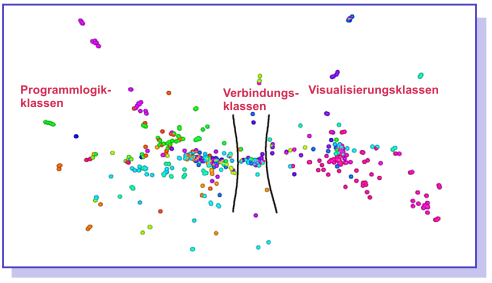
\includegraphics[width=0.85\textwidth]{3_1_1}
\end{figure}
\begin{figure}[h]
\centering
\caption{Ausschnitte der Programmlogik}
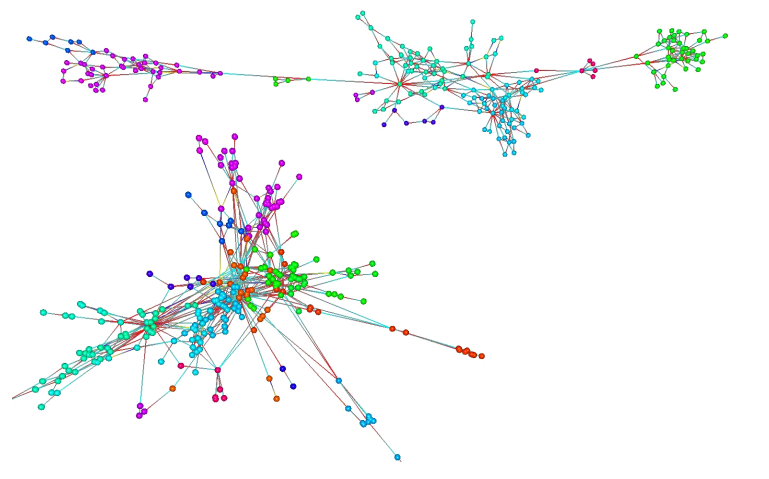
\includegraphics[width=0.85\textwidth]{3_1_2}
\end{figure}

\paragraph{Programmvisualisierung mit Doxygen und Graphviz:}
\begin{itemize}
	\item Doxygen generiert Programmdokumentation, Architekturdiagramme, etc.
	\item Graphviz (dot) ist ein Hilfsprogramm für Layoutberechnung;
\end{itemize}

\subsection{Strukturierte Gruppenprüfungen (Reviews)}
Systematische Verfahren zur gemeinsamen „Durchsicht“ von Dokumenten (wie z.B. erstellte UML-Modelle, implementierten Klassen, … ):
\begin{itemize}
	\item \textbf{Inspektion}: stark formalisiertes Verfahren bei dem Dokument nach genau festgelegter Vorgehensweise durch Gutachterteam untersucht wird
	\item \textbf{Technisches Review}: weniger formale manuelle Prüfmethode; weniger Aufwand als bei Inspektion, ähnlicher Nutzen
	\item \textbf{Informelles Review (Walkthrough)}: unstrukturiertere Vorgehensweise; Autor des Dokuments liest vor, Gutachter stellen spontane Fragen
	\item \textbf{Pair Programming}: Programm wird von vornherein zu zweit erstellt
\end{itemize}
Empirische Ergebnisse zu Programminspektion:
\begin{itemize}
\item Prüfaufwand liegt bei ca. 15 bis 20\% des Erstellungsaufwandes
\item 60 bis 70\% der Fehler in einem Dokument können gefunden werden
\item Nettonutzen: 20\% Ersparnis bei Entwicklung, 30\% bei Wartung
\end{itemize}

\paragraph{Psychologische Probleme bei Reviews:}
\begin{itemize}
	\item \textbf{-}: Entwickler sind in aller Regel von der Korrektheit der erzeugten Komponenten überzeugt (ihre Komponenten werden höchstens falsch benutzt)
	\item \textbf{-}: Komponententest wird als lästige Pflicht aufgefasst, die
	\begin{itemize}
		\item Folgearbeiten mit sich bringt (Fehlerbeseitigung) 
		\item Glauben in die eigene Unfehlbarkeit erschüttert
	\end{itemize}
	\item \textbf{-}: Entwickler will eigene Fehler (unbewusst) nicht finden und kann sie auch oft nicht finden (da ggf. sein Testcode von denselben falschen Annahmen ausgeht)
	\item \textbf{-}: Fehlersuche durch getrennte Testabteilung ist noch ärgerlicher (die sind zu doof zum Entwickeln und weisen mir permanent meine Fehlbarkeit nach)
	\item \textbf{+}: Inspektion und seine Varianten sind u.a. ein Versuch, diese psychologischen Probleme in den Griff zu bekommen
	\item \textbf{+}: Rolle des Moderators ist von entscheidender Bedeutung für konstruktiven Verlauf von Inspektionen
\end{itemize}

\paragraph{Vorgehensweise bei der Inspektion}
\begin{itemize}
	\item \textbf{Inspektionsteam} besteht aus Moderator, Autor (passiv), Gutachter(n), Protokollführer und ggf. Vorleser (nicht dabei sind Vorgesetzte des Autors / Manager)
	\item \textbf{Gutachter} sind in aller Regel selbst (in anderen Projekten) Entwickler
	\item Inspektion \textbf{überprüft}, ob:
	\begin{itemize}
		\item Dokument Spezifikation erfüllt (Implementierung konsistent zu Modell)
		\item für Dokumenterstellung vorgeschriebene Standards eingehalten wurden
	\end{itemize}
	\item Inspektion hat \textbf{nicht zum Ziel}:
	\begin{itemize}
		\item zu untersuchen, wie entdeckte Fehler behoben werden können
		\item Beurteilung der Fähigkeiten des Autors
		\item lange Diskussion, ob ein entdeckter Fehler tatsächlich ein Fehler ist
	\end{itemize}
	\item \textbf{Inspektionsergebnis:}
	\begin{itemize}
		\item formalisiertes Inspektionsprotokoll mit Fehlerklassifizierung
		\item Fehlerstatistiken zur Verbesserung des Entwicklungsprozesses
	\end{itemize}
\end{itemize}

\paragraph{Ablauf einer Inspektion:}
\begin{itemize}
	\item \textbf{Planung} des gesamten Verfahrens durch Management und Moderator
	\item \textbf{Auslösung} der Inspektion durch Autor eines Dokumentes (z.B. durch Freigabe)
	\item \textbf{Eingangsprüfung} durch Moderator (bei vielen offensichtlichen Fehlern wird das Dokument sofort zurückgewiesen) 
	\item \textbf{Einführungssitzung}, bei der Prüfling den Gutachtern vorgestellt wird
	\item \textbf{Individualuntersuchung} des Prüflings (Ausschnitt) durch Gutachter (zur \textbf{Vorbereitung} auf gemeinsame Sitzung) anhand ausgeteilter Referenzdokumente 
	\item auf \textbf{Inspektionssitzung} werden Prüfergebnisse mitgeteilt und protokolliert sowie Prüfling gemeinsam untersucht
	\item \textbf{Nachbereitung} der Sitzung und  \textbf{Freigabe} des Prüflings durch Moderator (oder Rückgabe zur Überarbeitung)
\end{itemize}

\paragraph{Technisches Review (abgeschwächte Form der Inspektion):}
\begin{itemize}
	\item Prozessverbesserung und Erstellung von Statistiken steht nicht im Vordergrund
	\item Moderator gibt Prüfling nicht frei, sondern nur Empfehlung an Manager
	\item kein formaler Inspektionsplan mit wohldefinierten Inspektionsregeln
	\item Ggf. auch Diskussion alternativer Realisierungsansätze
\end{itemize}

\paragraph{Informelles Review (Walkthrough):}
\begin{itemize}
	\item Autor des Prüflings liest ihn vor (ablauforientiert im Falle von Software) 
	\item Gutachter versuchen beim Vorlesen ohne weitere Vorbereitung Fehler zu finden
	\item Autor entscheidet selbst über weitere Vorgehensweise
	\item Zielsetzungen:
	\begin{itemize}
		\item Fehler/Probleme im Prüfling identifizieren
		\item Ausbildung/Einarbeitung von Mitarbeitern
	\end{itemize}
\end{itemize}

\subsection{Kontroll- und Datenflussorientierte Analysen}
Der Kontrollflussgraph ist ... eine häufig verwendete Methode zur Darstellung von Programmen. ... Die Verarbeitungssteuerung übernehmen die Kontrollstrukturen der Software unter Nutzung der Datenwerte. Eingabedaten werden gelesen, um Zwischenergebnisse zu bestimmen, die in den Speicher geschrieben werden, ... . Die Daten „fließen“ quasi durch die Software; von Eingaben zu Ausgaben.
\\
Ein \textbf{gerichteter Graph} G ist ein Tupel (N,E) mit N, eine Menge von \textbf{Knoten} (Nodes) und E einer Menge gerichteter \textbf{Kanten} (Edges).

\paragraph{Kontrollflussgraph - formale Definition:}
Ein \textbf{Kontrollflussgraph} eines Programms (Prozedur) ist ein Gerichteter Graph $ G = (N, E, n_{start}, n_{final})$ mit 
\begin{itemize}
	\item $N$ ist die Menge der \textbf{Anweisungen} (Knoten) eines Programms
	\item $E \subseteq N x N$ ist die Menge der \textbf{Zweige} (Kanten) zwischen den Anweisungen des Programms
	\item $n_{start} \epsilon N $ ist der \textbf{Startknoten} des Programms
	\item $n_{end} \epsilon N $ ist der \textbf{Endknoten} des Programms
\end{itemize}
Es gilt für den Kontrollflussgraphen:
\begin{itemize}
	\item keine in den Startknoten einlaufenden Kanten
	\item keine aus dem Endknoten auslaufenden Kanten
\end{itemize}
Manchmal wird zusätzlich gefordert, dass Kontrollflussgraphen zusammenhängen sind:
\begin{itemize}
	\item es gibt einen Pfad von $n_{start}$ nach $n$
	\item es gibt einen Pfad von $n$ nach $n{final}$
\end{itemize}

\paragraph{Pfade im Kontrollflussgraphen - formale Definition}
Ein \textbf{Pfad der Länge k} in einem Kontrollflussgraphen ist eine Knotenfolge.
\\
Ein \textbf{zyklenfreier Pfad} enthält keinen Knoten zweimal.
\\
Ein \textbf{Zyklus} ist ein Pfad mit $n_{1} = n_{k}$.

\paragraph{Kontrollflussgraphsegmente - formale Definition}
Ein \textbf{Segment} oder \textbf{Block} eines Kontrollflussgraphen ist ein Knoten $s$, der einen Teilgraph ersetzt, der aus einem zyklenfreien Pfad besteht mit genau einer auslaufenden und einer einlaufenden Kante.

\paragraph{Datenflussattribute eines Kontrollflussgraphen}
Die Anweisungen eines Kontrollflussgraphen besitzen Datenflussattribute, die den Zugriffen auf Variable (Parameter,...) in den Anweisungen entsprechen:
\begin{itemize}
	\item $n \epsilon N$ besitzt das Attribut \textbf{def(v)} oder kurz \textbf{d(v)}, falls $n$ eine Zuweisung an $v$ enthält (Wert von $v$ definiert); \\
	gilt auch für Eingabeparameter bei $n_{start}$
	\item $n \epsilon N$ besitzt das Attribut \textbf{c-use(v)} oder kurz \textbf{c(v)}, falls $n$ eine Berechnung mit Zugriff auf $v$ enthält (c=compute); \\
	implizite Zuweisung an Ausgabeparameter am Ende ist auch c-use
	\item $n \epsilon N$ besitzt das Attribut \textbf{p-use(v)} oder kurz \textbf{p(v)}, falls n eine Fallentscheidung mit Zugriff auf $v$ enthält (p=predicative)
	\item $n \epsilon N$ besitzt das Attribut \textbf{r(v)}, falls es das Attribut \textbf{c(v)} oder \textbf{p(v)} besitzt, also lesend auf $v$ zugreift (r=reference); \\
	dient nur der Zusammenfassung von c(v) und p(v), wenn der Unterschied c/p irrelevant ist
	\item $n \epsilon N$ besitzt das Attribut \textbf{u(v)}, falls $v$ in dieser Anweisung (noch) keinen definierten Wert (mehr) besitzen kann
\end{itemize}

\paragraph{Kontrollflussgraphsegmente mit Datenflussattributen}
\begin{itemize}
	\item Sei s ein Kontrollflussgraphsegment mit Pfad $n_{start} = n_{1}, ..., n_{k} = n_{final}$ und $attr(n_{i})$ die Sequenz der Datenflussattribute der $n_{i}$. Dann ist $attr(s) := attr(n_{1}, ..., attr/n_{k})$ die Konkatenierung der Datenflussattributsequenzen von $n_1$ bis $n_k$
	\item Ein Knoten n mit einer Sequenz von Datenflussattributen $attr(n) := attr_{1}, ..., attr_{k}$ ist immer eine abkürzende Schreibweise für einen Pfad von Knoten $n_1, ..., n_{k}$, sodass jeder Knoten $n_{i}$ genau einen Datenflussattribut besitzt $attr(n_{i}) := attr_{i}$
	\item Allen folgenden Definitionen liegt immer ein ''segmentfreier'' Kontrollflussgraph zugrunde, in dem jeder Knoten genau ein Datenflussattribut besitzt
\end{itemize}

\paragraph{Inout-Parameterdiskussion und Aufruf von Prozeduren}
Die meisten Programmiersprachen erlauben \textbf{nicht} die Auszeichnung von Variablen, die reinen Ausgabeparameter-Charakter besitzen; in Pascal/Modula gibt es nur mit VAR gekennzeichnete \textbf{Inout-Parameter}, in Sprachen wie C oder C++ hat man nur die Möglichkeit, out-Parameter als Zeiger/Referenzen auf Variable/Objekte zu simulieren.
\\
\\
Für solche Parameter mit Ein- und Ausgabecharakter müssen wir wie folgt vorgehen:
\begin{itemize}
	\item Deklaration der Prozedur countVowels(IN s:...; INOUT count: ...): für $n_{start}$ wird d(count) sowie d(s) angenommen, da beide Variablen bei der Übergabe einen definierten Wert haben sollten. \\
	Für $n_{final}$ wird c(count) angenommen, da am Ende der Prozedur der Wert von count durch versteckte Zuweisung an Aufrufstelle übergeben wird.
	\item Aufruf der Prozedur countVowels(aSentence, aCounter): \\
	es wird c(aSentence) und c(aCounter) in normaler Anweisung oder p(aSentence) und p(aCounter) in Prädikat gefolgt von d(aCounter) angenommen, da beim Aufruf versteckte Zuweisungen die Werte von aSentence und aCounter an die Parameter s und count zuweisen
\end{itemize}

\paragraph{Felder, globale Variablen und Strukturen}
\begin{itemize}
	\item Zugriff auf \textbf{globale Variablen} in einer Prozedur (Methode): werden bei Ein- und Austritt aus der Prozedur ignoriert und ansonsten wie lokale Variablen behandelt
	\item Zugriff auf \textbf{Felder (Arrays)}:
	\begin{itemize}
		\item anArray[index] := ... wird als r(index) und d(anArray) gewertet
		\item .. := .. anArray[index] ... wird als r(index) und r(anArray) gewertet
	\end{itemize}
	\item Zugriff auf \textbf{Strukturen}: wenn notwendig, können die Bestandteile (Variablen) einer Struktur als einzelne Variablen behandelt werden
\end{itemize}

\paragraph{Datenflussgraph - formale Definition}
Ein \textbf{Datenflussgraph} $D = (V_{d}, E_{d})$ zu einem Kontrollflussgraphen G eines Programms besteht aus
\begin{itemize}
	\item einer Menge von Knoten $V_{d}$ für alle Anweisungen V des Programms
	\item einer Menge von \textbf{Datenflusskanten} $E_{d}$: \\
	$ (n_{1}, n_{2}) \epsilon E_{d} $ genau dann, wenn es einen Pfad p im Kontrollflussgraphen G von $n_{1}$ nach $n_{2}$ gibt, sodass für eine Variable/Parameter v gilt:
	\begin{enumerate}
		\item d(v) für $n_{1}$: Anweisung $n_{1}$ definiert Wert für v
		\item r(v) für $n_{2}$: Anweisung $n_{2}$ benutzt Wert von v
		\item für alle Anweisungen n auf Pfad p (ohne $n_{1}$), gilt nicht d(v) für n: \\
		n ändert also nicht den bei $n_{1}$ festgelegten Wert von v
	\end{enumerate}
\end{itemize}
Die Kanten des Datenflussgraphen verbinden also Zuweisungen an Variablen oder Parameter mit den Anweisungen, in denen die zugewiesenen Werte benutzt werden.

\paragraph{Programm-Slices zur Fehlersuche und Änderungsfolgeschätzung}
Ein \textbf{Abhängigkeitsgraph} $A = (N_{a}, E_{a})$ eines Programms ist ein gerichteter Graph, der
\begin{itemize}
	\item alle Knoten und Kanten des Datenflussgraphen enthält (ohne Zusammenfassung von Teilgraphen zu Segmenten) sowie zusätzlich
	\item Kanten (des Kontrollflussgraphen) von allen Bedingungen zu direkt kontrollierten Anweisungen (das sind die Anweisungen, deren Ausführung von der Auswertung des betrachteten Bedingung abhängt).
\end{itemize}
Es gibt zwei Arten von Ausschnitten (Slices) eines Abhängigkeitsgraphen A:
\begin{itemize}
	\item \textbf{Vorwärts-Slice} für Knoten $n \epsilon N_{a}$ mit Datenflussattribut d(v): \\
	alle Pfade in A, die von Knoten n ausgehen, der Variable v definiert (der Slice-Graph enthält alle Knoten und Kanten der Pfade)
	\begin{itemize}
		\item Ein Vorwärts-Slice zu einer Anweisung n, die einer Variable v einen Wert zuweist, bestimmt alle die Stellen eines Programms, die von einer Änderung des zugewiesenen Wertes (Berechnungsvorschrift) betroffen sein könnten.
		\item Ein Vorwärts-Slice dient der Abschätzung von Folgen einer Programmänderung.
	\end{itemize}
	\item \textbf{Rückwärts-Slice} für Knoten $n \epsilon N_{a}$ mit Datenflussattribut r(v): \\
	alle Pfade in A, die in Knoten n einlaufen, der Variable v referenziert (der Slice-Graph enthält alle Knoten und Kanten der Pfade)
	\begin{itemize}
		\item Ein \textbf{Rückwärts-Slice} zu einer Anweisung n, die eine Variable referenziert, bestimmt alle die Stellen eines Programms, die den Wert der Variable direkt oder indirekt bestimmt haben.
		\item Ein Rückwärts-Slice ist bei der Fehlersuche hilfreich, um schnell irrelevante Programmteile ausblenden zu können.
	\end{itemize}
\end{itemize}

\paragraph{Datenfluss- und Kontrollflussanomalien}
Eine \textbf{Anomalie} eines Programms ist eine verdächtige Stelle in dem Programm. Eine solche verdächtige Stelle ist keine garantiert fehlerhafte Stelle, aber eine potentiell fehlerhafte Stelle im Programm.
\\
\\
\textbf{Datenflussanomalien} (meist deutliche Hinweise auf Fehler) sind etwa:
\begin{itemize}
	\item es gibt einen Pfad im Kontrollflussgraphen, auf dem eine Variable v referenziert wird bevor sie zum ersten Mal definiert wird (Zugriff auf undefinierte Variable)
	\item es gibt einen Pfad im Kontrollflussgraphen, auf dem eine Variable v zweimal definiert wird ohne zwischen den Definitionsstellen referenziert zu werden (nutzlose Zuweisung an Variable)
\end{itemize}
Kontrollflussanomalien sind bei modernen Programmiersprachen von geringerer Bedeutung. Im wesentlichen handelt es sich dabei bei Programmiersprachen ohne ''goto''-Anweisungen um nicht erreichbaren Code (ansonsten beispielsweise Sprünge in Schleifen hinein).

\paragraph{Undefined-Reference-Datenflussanomalie:}
Eine \textbf{ur-Datenflussanomalie} bezüglich einer 
Variable v ist wie folgt definiert:
\begin{itemize}
	\item es gibt einen segmentfreien Pfad $n_{1}, ... n_{k}$
	\item $n_{1}$ hat Attribut u(v), v besitzt also keinen definierten Wert bei $n_{1}$
	\item $n_{2}, ... n_{k-1}$ hat nicht Attribut d(v), v erhält also keinen definierten Wert
	\item $n_{k}$ hat Attribut r(v), auf v wird also lesend zugegriffen
\end{itemize}

\paragraph{Defined-Defined-Datenflussanomalie:}
Eine \textbf{dd-Datenflussanomalie} bezüglich einer Variable v ist wie folgt definiert:
\begin{itemize}
	\item es gibt einen segmentfreien Pfad $n_{1}, ... , n_{k}$
	\item $n_{1}$ hat Attribut d(v), v erhält also bei $n_{1}$ einen neuen Wert
	\item $n_{2}, ... , n_{k-1}$ hat nicht Attribut $[r|d|u](v)$, v wird also nicht bis $n_{k}$ verwendet
	\item $n_{k}$ hat Attribut d(v), alter Wert von v wird bei $n_{k}$ unbenutzt überschrieben
\end{itemize}

\paragraph{Defined-Undefined-Datenflussanomalie:}
Eine \textbf{du-Datenflussanomalie} bezüglich einer Variable v ist wie folgt definiert:
\begin{itemize}
	\item es gibt einen segmentfreien Pfad $n_{1}, ... , n_{k}$
	\item $n_{1}$ hat Attribut d(v), v erhält also einen definierten Wert bei $n_{1}$
	\item $n_{2}, ... , n_{k-1}$ hat nicht Attribut $[r|d|u](v)$, v wird also bis $n_{k}$ nicht verwendet
	\item $n_{k}$ hat Attribut u(v), v wird also auf undefiniert gesetzt
\end{itemize}

\paragraph{Probleme mit statischer Datenflussanalyse für Datenstrukturen}
\begin{itemize}
	\item Funktioniert nicht (gut) für komplexe Datenstrukturen wie Felder (Arrays), bei denen man jede einzelne Komponente wie eigene Variable behandeln müsste
	\item Noch größere Probleme hat man bei berzeigerten Datenstrukturen
	\item Unterscheidung von in-, out- und inout-Parametern (in Java, C++, ...)
\end{itemize}

\paragraph{Probleme mit statischer Datenflussanalyse bei Fallunterscheidungen}
Problem:
\begin{itemize}
	\item reale Programme enthalten oft viele Anomalien, die nicht echte Programmierfehler sind (zu viele nutzlose Warnungen werden erzeugt)
	\item restriktivere Definitionen von sogenannten starken Anomalien übersezen andererseits u.U. zu viele echte Fehler
\end{itemize}
Lösung:
\begin{itemize}
	\item zunächst neue Definitionen \textbf{''starker'' Anomalien} verwenden
	\item dann bisherige Definitionen von \textbf{(schwachen) Anomalien} verwenden
\end{itemize}

\paragraph{Definitionen starker Datenflussanomalien:}
\begin{itemize}
	\item \textbf{starke ur-Anomalie:} zu Anweisungen n mit Attribut u(v) und über einen Pfad von n erreichbarem n' mit r(v) gibt es \textbf{keinen} segmentfreien Pfad in G $n = n_{1}, ... , n_{k} = n'$ in dem $n'$ nur einmal auftritt und für den gilt: \\
	es existiert $i \epsilon 2, ... ,k-1$ mit $n_{i}$ besitzt Attribut d(v) oder u(v) \\
	\textbf{Idee dieser Definition:}
	\begin{itemize}
		\item von n mit u(v) nach $n'$ mit r(v) gibt es \textbf{mindestens} einen Ausführungspfad
		\item ausgeschlossen werden \textbf{zyklische Pfade} durch n', um so die Analyse auf die erste Ausführung einer Anweisung in einer Schleife einzuschränken
		\item auf \textbf{keinem} Pfad wird an Variable v ein Wert zugewiesen, bevor bei n' lesend auf v zugegriffen wird
		\item des weiteren werden Situationen ausgeschlossen, bei denen die gerade betrachtete ur-Anomalie (teilweise) durch irgendeine andere Anomalie ''\textbf{überlagert}'' wird
	\end{itemize}
	\item \textbf{starke du-Anomalie:} zu Anweisungen n mit Attribut d(v) und über einen Pfad von n erreichbarem n' mit u(v) gibt es \textbf{keinen} segmentfreien Pfad in G $n = n_{1}, ... , n_{k} = n'$ in dem n' nur einmal auftritt und für den gilt: \\
	es existiert $i \epsilon 2, ... , k-1$ mit: $n_{i}$ besitzt Attribut d(v) oder u(v) oder r(v) \\
	\textbf{Idee dieser Definition:}
	\begin{itemize}
		\item von n mit d(v) nach n' mit u(v) gibt es \textbf{mindestens} einen Ausführungspfad
		\item ausgeschlossen werden wieder \textbf{bestimmte Zyklen}, um so die Analyse auf die erste Ausführung einer Anweisung in einer Schleife einzuschränken
		\item auf \textbf{keinem} Pfad wird an Variable v bei n zugewiesener Wert verwendet, bevor er bei n' undefiniert wird
		\item des weiteren werden Situationen ausgeschlossen, bei denen die gerade betrachtete du-Anomalie (teilweise) durch irgendeine andere Anomalie ''\textbf{überlagert}'' wird
	\end{itemize}
	\item \textbf{starke dd-Anomalie:} zu Anweisungen n mit Attribut d(v) und über einen Pfad von n erreichbarem n' mit d(v) gibt es \textbf{keinen} segmentfreien Pfad in G $n = n_{1}, ... , n_{k} = n'$ in dem n' nach $n_{1}$ nur einmal auftritt und für den gilt \\
	es existiert $i \epsilon 2, ... ,k-1$ mit: $n_{i}$ besitzt Attribut d(v) oder u(v) oder r(v) \\
	\textbf{Idee dieser Definition:}
	\begin{itemize}
		\item von n mit d(v) nach n' mit d(v) gibt es \textbf{mindestens} einen Ausführungspfad
		\item ausgeschlossen werden wieder \textbf{bestimmte Zyklen}, um so die Analyse auf die erste Ausführung einer Anweisung in einer Schleife einzuschränken 
		\item auf \textbf{keinem} Pfad wird an Variable v bei n zugewiesener Wert verwendet, bevor bei n' erneut ein Wert zugewiesen wird
		\item des weiteren werden Situationen ausgeschlossen, bei denen die gerade betrachtete dd-Anomalie (teilweise) durch irgendeine andere Anomalie ''\textbf{überlagert}'' wird
	\end{itemize}
\end{itemize}

\subsection{Softwaremetriken}

Die Definition von Software-Maßen basiert auf dem Wunsch, einen quantitativen Zugang zum abstrakten Produkt Software zu gewinnen. Dabei ist zwischen der Vermessung von Eigenschaften einer Software und der quantitativen Kontrolle des zugrundeliegenden Entwicklungsprozesses zu unterscheiden
\begin{itemize}
	\item \textbf{Produktmetriken} messen Eigenschaften der Software
	\begin{itemize}
		\item Qualität der Software (z.B. Anzahl der gefundenen Fehler)
		\item Einhaltung von Standards (z.B. als Anzahl Verletzung von Stilregeln)
	\end{itemize}
	\item \textbf{Prozessmetriken} messen Eigenschaften des Entwicklungsprozesses:
	\begin{itemize}
		\item Dauer oder Kosten der Entwicklung (z.B. als Mitarbeitermonate)
		\item Zufriedenheit des Kunden (z.B. als Anzahl Änderungswünsche)
	\end{itemize}
\end{itemize}

\paragraph{Gewünschte Eigenschaften von Maß/Metrik}
\begin{itemize}
	\item \textbf{Einfachheit}: berechnetes Maß lässt sich einfach interpretieren (z.B. Zeilenzahl einer Datei)
	\item \textbf{Eignung} (Validität):  es besteht ein (einfacher) Zusammenhang zwischen der gemessenen Eigenschaft und der interessanten Eigenschaft (z.B. zwischen Programmlänge und Fehleranzahl)
	\item \textbf{Stabilität}:  gemessene Werte sind stabil gegenüber Manipulationen untergeordneter Bedeutung (z.B. die Unterschiede zwischen zwei Projekten, wenn man aus erstem Projekt Rückschlüsse auf zweites Projekt ziehen will)
	\item \textbf{Rechtzeitigkeit}: das Maß kann zu einem Zeitpunkt berechnet werden, zu dem es noch zur Steuerung des Entwicklungsprozesses hilfreich ist (Gegenbeispiel: Programmlänge als Maß für Schätzung des Entwicklungsaufwandes)
	\item \textbf{Reproduzierbarkeit}: am besten automatisch berechenbar ohne subjektive Einflussnahme des Messenden (Gegenbeispiel: Beurteilung der Lesbarkeit eines Programms durch manuelle Durchsicht)
\end{itemize}

\paragraph{Maßskalen:}
\begin{itemize}
	\item \textbf{Nominalskala}: frei gewählte Menge von Bezeichnungen wie etwa Programm in C++, Java, Fortran, ... geschrieben 
	\item \textbf{Ordinalskala}: geordnete Menge von Bezeichnern wie etwa Programm gut lesbar, einigermaßen lesbar, ... , absolut grauenhaft
	\item \textbf{Rationalskala}: Messwerte können zueinander in Relation gesetzt werden und prozentuale Aussagen mit Multiplikation und Division sind sinnvoll wie etwa Programm A besitzt doppelt/halb so viele Programmzeilen wie Programm B
\end{itemize}

\paragraph{Berechnung der Regressionsgeraden:}
Gesucht wird: $Y=b_{0}+b_{1}X$ \\
Gegeben sind paare von Messwerten: $(x_{1},y_{1}),...,(x_{n},y_{n})$
Berechnung der Mittelwerte. \\
Berechnung von Koeffizient $b_{1}$:
\begin{equation}
b_{1}=\frac{\frac{1}{n-1}\cdot\sum_{i=1}^{n}(x_{i}-\overline{x})(y_{i}-\overline{y})}{\frac{1}{n-1}\sum_{i=1}^{n}(x_{i}-\overline{x})^2} = \frac{\sum_{i=1}^{n}(x_{i}-\overline{x})(y_{i}-\overline{y})}{\sum_{i=1}^{n}(x_{i}-\overline{x})^2}
\end{equation}
Berechnung von Koeffizient $b_{0}$: $b_{0} = \overline{y} - b_{1}\overline{x}$

\paragraph{Berechnung des Korrelationskoeffizienten r:}

\begin{equation}
	r = \frac{\sum_{i=1}^{n}(x_{i}-\overline{x})\cdot(y_{i}-\overline{y})}{\sqrt{\sum_{i=1}^{n}(x_{i}-\overline{x})^2\cdot\sum_{i=1}^{n}(y_{i}-\overline{y})^2}}
\end{equation}

\begin{itemize}
	\item man kann zeigen, dass der \textbf{Korrelationskoeffizient} $r \epsilon [-1...+1]$ gilt
	\item die Grenzfälle $r=+1$ und $e=-1$ treten auf, wenn schon alle gemessenen Punkte $(x_{i},y_{i})$ auf einer Gerade liegen
	\item die Regressionsgerade steigt für $r=+1$ und fällt für $r=-1$
	\item für $r=0$ verläuft die Gerade parallel zur X-Achse, es besteht also kein (linearer) Zusammenhang zwischen X- und >-Werten
	\item $r^2$ heißt \textbf{Bestimmtheitsmaß} und lässt sich interpretieren als Anteil der durch die Regression erklärten Streuung der Y-Werte
	\item hat man z.B. r=0.7 erhalten, dann ist $r^2=0.49$ der Streuung der Y-Werte werden durch die lineare Abhängigkeit von X erklärt
\end{itemize}

\paragraph{Auswertung von ordinalen/rationalen Metriken:}
\begin{enumerate}
	\item augrund von Erfahrungswerten sind sinnvolle untere und obere Grenzwerte für einen Messwert bekannt
	\begin{itemize}
		\item alle Komponenten (Module, Klassen, Methoden,...) mit kritischen Werten werden genauer untersucht und ggf. saniert(neu geschrieben)
	\end{itemize}
	\item solche Grenzwerte für Messergebnisse sind nicht bekannt
	\begin{itemize}
		\item alle Komponenten (Module, Klassen, Methoden,...) werden untersucht, deren Messwerte außerhalb des Bereichs liegen, in dem 95\% der Messwerte liegen (oder 80\% oder...)
	\end{itemize}
	\item funktionaler Zusammenhang zwischen Metrik und gewünschtem Qualitätsmerkmal genauer bekannt
	\begin{itemize}
		\item zulässige Werte für Metrik werden aus Qualitätsanforderungen errechnet (ein Wunschtraum...)
	\end{itemize}
	
\end{enumerate}

\paragraph{Gleichzeitige Darstellung mehrerer Messwerte mit Kiviatdiagramm}

\begin{figure}[h]
	\centering
	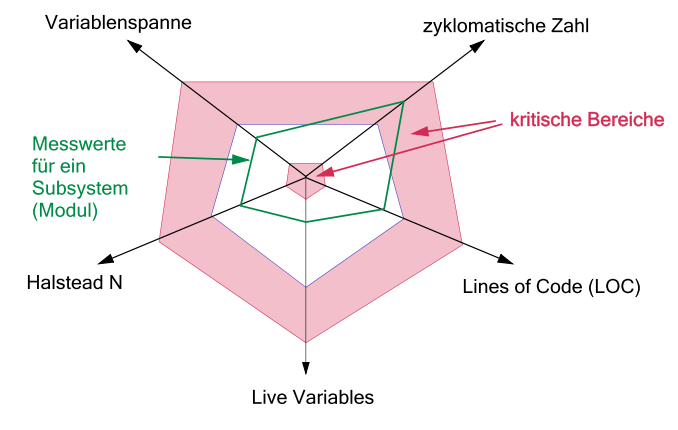
\includegraphics[width=0.85\textwidth]{3_1_3}
\end{figure}

\paragraph{Lines of Code = LOC}

LOC ist die naheliegendste Metrik. Festlegung des LOC:
\begin{itemize}
	\item Anzahl aller Zeilen der Textdatei(en) des betrachteten Programmteils
	\item Anzahl Zeilen der Textdatei(en) ohne Kommentare und Leerzeilen
	\item Anzahl Trennzeichen zwischen Anweisungen, also '';'' oder ...
	\item Anzahl Trennzeichen wie '';'' plus Schlüsselwörter wie ''IF'',...
	\item Knoten im Kontrollflussgraphen
	\item Programmlänge nach Halstead
\end{itemize}

\paragraph{LOC(Programmteil) = Anzahl der Knoten im Kontrollflussgraphen} 
Idee dieser Maßzahl:
\begin{itemize}
	\item betrachtete Programmteile oder ganze Programme mit hoher LOC sind zu komplex (no separation of concerns) und deshalb fehlerträchtig
	\item Programmteile mit geringer LOC sind zu klein und führen zu unnötigen Schnittstellenproblemen
\end{itemize}
Probleme mit dieser Maßzahl:
\begin{itemize}
	\item Kanten = Kontrollflusslogik spielen keine Rolle
	\item wie bewertet man geerbten Code einer Klasse
\end{itemize}

\paragraph{Zyklomatische Zahl(Komplexität) nach McCabe:}
\textbf{ZZ(Programmteil) = |E| - |N| + 2k} mit G als Kontrollflussgraph des Untersuchten Programmteils und
\begin{itemize}
	\item |E|:= Anzahl Kanten von G
	\item |N|:= Anzahl Knoten von G
	\item k:= Anzahl Zusammenhangskomponenten von G (Anzahl der nicht miteinander verbundenen Teilgraphen von G)
\end{itemize}

\textbf{Regel von McCabe:} ZZ eines in sich abgeschlossenen Teilprogramms (Zusammenhangskomponente) sollte nicht höher als 10 sein, da sonst Programm zu komplex und zu schwer zu testen ist

\paragraph{Interpretation und Probleme mit der zyklomatischen Zahl (Komplexität):}

\begin{itemize}
	\item es wird die Anzahl der Verzweigungen (unabhängigen Pfade) in einem Programm gemessen
	\begin{itemize}
		\item es wird davon ausgegangen, dass jede Zusammenhangskomponente (Teilprogramm) genau einen Eintritts- und einen Austrittsknoten hat
		\item damit besitzt jede Zusammenhangskomponente mit n Knoten mindestens n-1 Kanten; diese immer vorhandenen Kanten werden nicht mitgezählt
		\item die kleinste Komplexität einer Zusammenhangskomponente soll 1 sein, also wird von der Anzahl der Kanten n abgezogen und 2 addiert
	\end{itemize}
	\item in GOTO-freien Programmen wird damit genau die Anzahl der bedingten Anweisungen und Schleifen (if/while-Statements) gemessen
	\item die Zahl ändert sich nicht beim Einfügen normaler Anweisungen
	\item deshalb ist die Regel von McCabe mit \textbf{ZZ(Komponente) < 11} umstritten, da allenfalls eine Aussage über Testaufwand (Anzahl der zu testenden unabhängigen Programmpfade) getroffen wird
\end{itemize}

\paragraph{Halstead-Metriken - Eingangsgrößen:}

Die Halstead-Metriken messen verschiedene Eigenschaften einer Software-komponente. Als Eingabe dienen immer:
\begin{itemize}
	\item $\eta_{1}$: Anzahl der unterschiedlichen Operatoren eines Programms (verwendete arithmetische Operatoren, Prozeduren, Methoden, ... )
	\item $\eta_{2}$: Anzahl der unterschiedlichen Operanden eines Programms (verwendete Variablen, Parameter, Konstanten, ... )
	\item $N_{1}$: Gesamtzahl der verwendeten Operatoren in einem Programm (jede Verwendungsstelle wird separat gezählt)
	\item $N_{2}$:  Gesamtzahl der verwendeten Operanden in einem Programm (jede Verwendungsstelle wird separat gezählt)
	\item $\eta := \eta_{1}+\eta_{2}$:  Anzahl der verwendeten Deklarationen \textbf{(Programmvokabular)}
	\item $N := N_{1} + N_{2}$:Anzahl der angewandten Auftreten von Deklarationen (wird auch „normale“ Programmlänge genannt)
\end{itemize}

In der Literatur vorgeschlagene Zählregeln für Operatoren in Java:
\begin{itemize}
	\item Arithmetische und logische Standardoperatoren
	\item Sonderzweichen (Zuweisung, Konkatenation, Attributselektion)
	\item Reservierte Java-Schlüsselwörter
	\item Definitionen von Methoden und Funktionen
\end{itemize}

\paragraph{Halstead-Metriken - Definition:}
\begin{enumerate}
	\item \textbf{Berechnete Programmlänge} $L := \eta_{1}log_{2}\eta_{1} + \eta_{2}log_{2}\eta_{2}$ (hängt also nur von Anzahl verwendeter Operatoren und Operanden ab; postuliert wird, dass man  mit einer festen Anzahl von Operatoren und Operanden immer Programme einer bestimmten logischen Größe schreibt)
	\item \textbf{Programmgröße} $V=N log_{2} \eta$ (Programme Volume) (optimale Codierung des Programms als Bitvektor)
	\item ...
\end{enumerate}

\textbf{Bewertung:} Es gibt eine ganze Reihe weiterer Halstead-Metriken, deren Nutzen umstritten ist, und die versuchen zu bewerten:
\begin{itemize}
	\item \textbf{Schwierigkeit} der Erstellung eines Programms
	\item \textbf{Adäquatheit} einer bestimmten Programmiersprache für Problemstellung
	\item \textbf{Aufwand} für Erstellung eines Programms
\end{itemize}

\paragraph{''Live Variable''-Definition:}
Die \textbf{''Live Variables''}-Metrik berechnet für eine Programmkomponente die durchschnittliche Anzahl lebendiger Variablen dieser Komponente je Knoten des zugehörigen Kontrollflussgraphen; eine Variable ist dabei von ihrer ersten Definitionsstelle (vom Startknoten aus) bis zur letzten Definitions- oder Referenzierungsstelle (vor dem Endknoten) \textbf{lebendig}. 
\\
\\
\textbf{Zusammenfassung:} Live Variables einer Komponente ist durchschnittliche Anzahl lebendiger Variablen in einem Programm pro Zeile (Knoten im Kontrollflussgraphen). Eine Variable ist von ihrer ersten Definitionsstelle (vom Startknoten aus) bis zur letzten Definitions- oder Referenzierungsstelle (vor dem Endknoten) lebendig.

\paragraph{''Variablenspanne''-Definition:}

Die \textbf{''Variablenspannen''}-Metrik einer Programmkomponente berechnet die durchschnittliche Spanne zweier direkt aufeinander folgender definierender oder referenzierender Auftreten derselben Variable im zugehörigen Kontrollflussgraphen; die Spanne zweier Knoten in einem Kontrollflussgraphen entspricht der Länge des kürzesten Pfades (Anzahl Kanten dieses Pfades) zwischen diesen beiden Knoten.
\\
\\
\textbf{Zusammenfassung:} Variablenspanne einer Komponente ist die durchschnittliche Spanne zweier direkt aufeinander folgender definierender oder referenzierender Auftreten derselben Variable

\paragraph{Anmerkung zu Live Variables und Variablenspanne:}

Mit diesen beiden Metriken versucht man nicht die ''Kontrollflusskomplexität'' oder einfache Größe einer Softwarekomponente, sondern die Komplexität des Datenflusses zu bewerten (wieviele Variablen muss man wie lange beim Erstellen von Programmteilen oder beim Nachvollziehen des Programmablaufs ''im Kopf behalten'').

\paragraph{Überlegungen zu Metriken für objektorientierte Programme:}

Betrachtet wird oft Kopplung von Klassen = Benutzt-Beziehungen zwischen Klassen:
\begin{itemize}
	\item \textbf{geringer fan-out} (wenige auslaufende Benutzt-Beziehungen) ist positiv, da sich dann eine Klasse auf wenige andere Klassen abstützt
	\item \textbf{hoher fan-in} (viele einlaufende Benutzt-Beziehungen) ist positiv, da dann eine Klasse von vielen Klassen (wieder-)verwendet wird
	\item beides kann nicht maximiert werden, da über alle Klassen hinweg gilt: \textbf{Summe fan-in = Summe fan-out}
\end{itemize}
Eine Klasse A benutzt eine Klasse B, wenn:
\begin{itemize}
	\item in A ein Verweis auf Objekt der Klasse B verwendet wird
	\item in A eine Operation einen Parameter der Klasse B verwendet
	\item in A eine Operation der Klasse B aufgerufen wird
\end{itemize}
Gesucht werden Metriken, die neben der Kopplung von Klassen folgende Aspekte in Maßzahlen zusammenfassen:
\begin{itemize}
	\item die Methoden einer Klasse sollten \textbf{enge Bindung (high cohesion)} besitzen, also einem ähnlichen Zweck dienen (wie misst man das?)
	\item die Klassen einer Vererbungshierarchie sollten ebenfalls \textbf{enge Bindung} besitzen
	\item die in einem Modul bzw. Paket zusammengefassten Klassen oder die in einer Klasse zusammengefassten Methoden sollten \textbf{enge Bindung} besitzen
	\item Klassen in verschiedenen Modulen bzw. Paketen sollte lose gekoppelt sein (wie misst man das?) \textbf{(loose coupling)}
	\item Klassen und Module bzw. Pakete sollten ein Implementierungsgeheimnis verbergen \textbf{(data abstraction, encapsulation)} 
	\item ...
\end{itemize}

\paragraph{Bindungsmetriken - LOCOM (Low Cohesion Metric)}
Die Bindung der Methoden einer Klasse wird untersucht. Methoden sind eng miteinander gebunden, wenn sie auf viele gemeinsame Attribute oder Felder zugreifen. 
\\
\\

\textbf{LOCOM1}
\begin{itemize}
	\item P := Anzahl der Paare von Methoden ohne gemeinsame Attributzugriffe
	\item  := Anzahl der Paare von Methoden mit gemeinsamen Attributzugriffen
	\item LOCOM1 := if P>Q then P-Q else 0
	\item Gewünscht wird Wert von LOCOM1 nahe 0
\end{itemize}
\textbf{LOCOM2}
\begin{itemize}
\item m := Anzahl Methoden $m_{i}$ einer Klasse \\
$m(a_{i})$ := Anzahl Methoden die auf Attribut $a_{i}$ zugreifen
\item  n := Anzahl Attribute $a_{i}$ einer Klasse
\item LOCOM1 := 1 - (m($a_{1}$)+...+m($a_{n}$))/(m*n)
\item Gewünscht wird kleiner Wert von LOCOM2
\end{itemize}

\paragraph{Weitere Metriken}
\begin{itemize}
	\item \textbf{Afferent Coupling (Ca/AC)}: Die Anzahl der Klassen ausserhalb eines betrachteten Teilsystems (Kategorie), die von den Klassen innerhalb des Teilsystems abhängen
	\item \textbf{Efferent Coupling (Ce/EC):} Die Anzahl der Klassen innerhalb eines betrachteten Teilsystems (Kategorie), die von Klassen ausserhalb des betrachteten Teilsystems abhängen
	\item \textbf{Instabilität (I)}:   I = Ce / (Ce+Ca)
	\begin{itemize}
		\item I hat einen Wert zwischen 0 und 1, falls nicht Ce + Ca = 0 gilt mit 0 = max. stabil u. 1 = max. unstabil
		\item der Wert 1 besagt, dass Ca = 0 ist; das betrachtete Teilsystem exportiert also nichts nach außen (keine Klassen und deren Methoden) 
		\item der Wert 0 besagt, dass Ce = 0 ist; das betrachtete Teilsystem importiert also nichts von außen (keine Klassen und deren Methoden)
		\item Der ''undefinierte'' Fall Ca = 0 und Ce = 0 kann nur auf ein (sinnloses) isoliertes Teilsystem zutreffen, das weder importiert noch exportiert 
	\end{itemize}
	\item \textbf{Coupling als Change Dependency between Classes (CDBC)}. CDBC bewertet Aufwand, der mit Überarbeitung von CC wegen Änderung in SC verbunden sein könnte (Anzahl potentiell zu überarbeitender Methoden in CC).
	\begin{itemize}
		\item  n falls SC Oberklasse von CC ist (n = Anzahl Methoden in CC)
		\item n falls CC ein Attribut des Typs SC hat
		\item j falls SC in j Methoden von CC benutzt wird (als Typ lokaler Variable, Parameter oder Methodenaufruf von SC)
	\end{itemize}
	\item \textbf{Encapsulation als Attribute Hiding Factor (AHF)}.
	\begin{itemize}
		\item Sind alle Attribute als „private“ definiert, dann ist AHF = 1.
		\item Summe der Unsichtbarkeiten aller Attribute in allen Klassen geteilt durch die Anzahl aller Attribute
		\item Unsichtbarkeit eines Attributs := Prozentzahl der Klassen, für die das Attribut nicht sichtbar ist (abgesehen von eigener Klasse)
	\end{itemize}
	\item \textbf{Tiefe von Vererbungshierarchien:} zu tiefe Hierarchien werden unübersichtlich; man weiss nicht mehr, was man erbt
	\item \textbf{Breite von Vererbungshierarchien:} zu breite Vererbungshierarchien deuten auf Fehlen von zusammenfassenden Klassen hin
	\item \textbf{Anzahl Redefinitionen in einer Klassenhierarchie:} je mehr desto gefährlicher
	\item \textbf{Anzahl Zugriffe auf geerbte Attribute:} sind ebenfalls gefährlich, da beim Ändern von Attributen oder Attributzugriffen in Oberklasse die Zugriffen in den Unterklassen oft vergessen werden
\end{itemize}

\paragraph{Komplexitätsmaße:}
\begin{itemize}
	\item \textbf{Response for Class (RFC):}
	die Anzahl der in der Klasse deklarierten Methoden + die Anzahl der geerbten Methoden + die Anzahl sichtbarer Methoden anderer Klassen (Alle Methoden, die aufgerufen werden können? Sehr schwammig definiert!!!)
	\item \textbf{Weighted Methods Per Class (WMPC1):} \\
	die Summe der zyklomatischen Zahlen ZZ aller Methoden der Klasse (ohne geerbte Methoden)
	\item \textbf{Number of Remote Methods (NORM):}
	die Anzahl der in einer Klasse gerufenen Methoden ''fremder'' Klassen (also nicht die Klasse selbst oder eine ihrer Oberklassen)
	\item \textbf{Attribute Complexity (AC):}
	die gewichtete Summe der Attribute einer Klasse wird gebildet; Gewichte werden gemäß Typen/Klassen der Attribute vergeben. 
\end{itemize}


\subsection{Zusammenfassung}
Die \textbf{Visualisierung von Software} ist sowohl beim ''Forward Engineering'' für den Entwurf neuer Programmarchitekturen als auch beim „Reverse Engineering“ für das Studium von ''Legacy Software'' mit unbekannter Programmstruktur sehr hilfreich.
\\
\\
Werkzeugunterstützte \textbf{statische Analyseverfahren} helfen frühzeitig bei der Identifikation kritischer Programmstellen. Es sollten folgende Analyseverfahren immer eingesetzt werden:
\begin{itemize}
	\item \textbf{Stilanalyse} (Überprüfung vereinbarter Programmierkonventionen)
	\item \textbf{''dead code''-Analyse} (oft in Compiler eingebaut): nie verwendete Methoden, Variablen, Parameter, ... (wurde bisher nicht angesprochen)
	\item \textbf{Datenflussanalyse} (wenn Werkzeug verfügbar)
\end{itemize}
Weitere Analyseverfahren und vor allem \textbf{Metriken} sollten in großen Projekten zumindest versuchsweise eingesetzt werden.

\paragraph{Vorgehensweise beim Einsatz von Maßen}
\begin{enumerate}
	\item Fragen zur Ausgangssituation
	\begin{itemize}
		\item  In welcher Phase (Aktivitätsbereich) des Softwareentwicklungsprozesses soll eine Verbesserung eingeführt werden (z.B. Design, Codierung, ... )?
		\item Was soll damit erreicht werden bzw. welche Art von Fehler soll reduziert werden (z.B. Reduktion C++ Codierungsfehler)?
		\item Welche Methode soll eingesetzt werden (z.B. OO-Metriken)?
		\item Welche Technik/Werkzeug soll eingesetzt werden
	\end{itemize}
	\item \textbf{Bewertung des aktuellen Standes} des Entwicklungsprozesses:
	\begin{itemize}
		\item Welche Kosten u. welcher Aufwand entstehen  in welcher Phase?
		\item Wie ist die Qualität  der Ergebnisse jeder Phase?
		\item In welcher Phase entsteht welcher Anteil an Fehlern und welcher Teil der Fehlerbeseitigungskosten?
	\end{itemize}
	\item Mittel zur Bestimmung des aktuellen Standes, \textbf{zu messende Aspekte:}
	\begin{itemize}
		\item Kosten- und Zeitverfolgung beim Entwicklungsprozess
		\item  Definition von Qualitätsmaßen für Produkt pro Phase
		\item Erhebung von Fehlerstatistiken
	\end{itemize}
	\item \textbf{Analyse der Ergebnisse} und Erarbeitung von Verbesserungsvorschlägen:
	\begin{itemize}
		\item Auswertung der Maße
		\item Definition von Zielen auf Basis der Messwerte
		\item Entscheidung für Verbesserung in bestimmten Phasen
		\item Auswahl geeigneter Methoden und Werkzeuge
		\item Einführung der Methoden und Werkzeuge in Entwicklungsprozess
	\end{itemize}
	\item Bewertung der durchgeführten Änderungen:
	\begin{itemize}
		\item Kontinuierliche Weiterauswertung der Maße
		\item erneute Analyse nach ''Abklingen von Einschwingvorgängen''
	\end{itemize}
\end{enumerate}










	\section{Dynamische Programmanalysen und Testen}
The older I get, the more aggressive I get about testing. I like Kent Beck’s rule of thumb that a developer should write at least as much test code as production code. Testing should be a continuous process. No code should be written until you know how to test it. Once you have written it, write the tests for it. Until the test works, you cannot claim to have finished writing the code.

\subsection{Einleitung}

\begin{figure}[h]
	\centering
	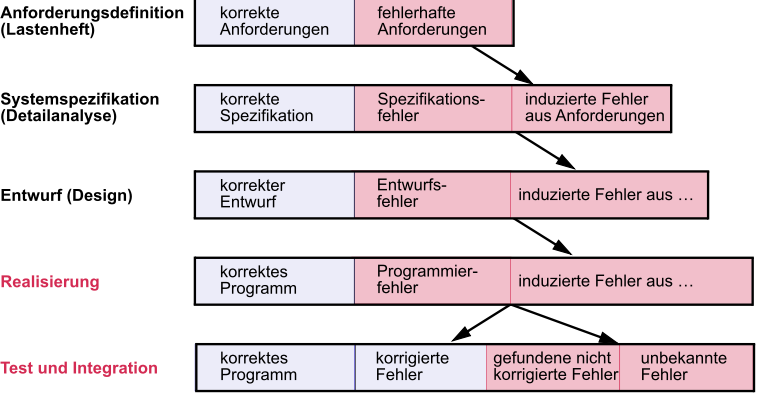
\includegraphics[width=0.85\textwidth]{4_1}
\end{figure}

\paragraph{Fehlerzustand, Fehlerwirkung und Fehlhandlung (DIN 66271):}

\begin{itemize}
	\item \textbf{Fehlerzustand (fault) - direkt erkennbar durch statische Tests: }
	\begin{itemize}
		\item inkorrektes Teilprogramm, inkorrekte Anweisung oder Datendefinition, die Ursache für Fehlerwirkung ist
		\item Zustand eines Softwareprodukts oder einer seiner Komponenten, der unter spezifischen Bedingungen eine geforderte Funktion beeinträchtigen kann
	\end{itemize}
	\item \textbf{Fehlerwirkung (failure) - direkt erkennbar durch dynamische Tests: }
	\begin{itemize}
		\item Wirkung eines Fehlerzustandes, die bei der Ausführung des Testobjektes nach ''außen'' in Erscheinung tritt
		\item Abweichung zwischen spezifiziertem Soll-Wert (Anforderungsdefinition) und beobachtetem Ist-Wert (bzw. Soll- und Ist-Verhalten)
	\end{itemize}
	\item \textbf{Fehlhandlung (error): }
	\begin{itemize}
		\item menschliche Handlung (des Entwicklers), die zu einem Fehlerzustand in der Software führt
		\item \textbf{NICHT einbezogen:} menschliche Handlung eines Anwenders, die ein unerwünschtes Ergebnis zur Folge hat
	\end{itemize}
\end{itemize}

\paragraph{Ursachenkette für Fehler (in Anlehnung an DIN 66271):}

\begin{itemize}
	\item jeder Fehler (\textbf{fault}) oder Mangel ist seit dem Zeitpunkt der Entwicklung in der Software vorhanden - Software nützt sich nicht ab
	\item er ist aufgrund des fehlerhaften Verhaltens (\textbf{error}) eines Entwicklers entstanden (und wegen mangelhafter Qualitätssicherungsmaßnahmen nicht entdeckt worden)
	\item ein Softwarefehler kommt nur bei der Ausführung der Software als Fehlerwirkung (\textbf{failure}) zum Tragen und führt dann zu einer ggf. sichtbaren Abweichung des tatsächlichen Programmverhaltens vom gewünschten Programmverhalten
	\item Fehler in einem Programm können durch andere Fehler \textbf{maskiert} werden und kommen somit ggf. nie zum Tragen (bis diese anderen Fehler behoben sind)
\end{itemize}

\paragraph{Validation und Verifikation (durch dynamische Tests):}
\begin{itemize}
	\item \textbf{Validation von Software: }
	\begin{itemize}
		\item Prüfung, ob die Software das vom Anwender „wirklich“ gewünschte Verhalten zeigt (in einem bestimmten Anwendungsszenario)
		\item Haben wir das richtige Softwaresystem realisiert?
	\end{itemize}
	\item \textbf{Verifikation von Software: }
	\begin{itemize}
		\item Prüfung, ob die Implementierung der Software die Anforderungen erfüllt, die vorab (vertraglich) festgelegt wurden
		\item Haben wir das Softwaresystem richtig realisiert?
	\end{itemize}
\end{itemize}
\textbf{Achtung:} Eine ''richtig realisierte'' = korrekte Software (erfüllt die spezifizierten Anforderungen) 
muss noch lange nicht das ''wirklich'' gewünschte Verhalten zeigen!

\paragraph{Typische Programmierfehler nach [BP84]:}

\begin{itemize}
	\item \textbf{Berechnungsfehler}: Komponente berechnet falsche Funktion
	\begin{itemize}
		\item z.B. Konvertierungsfehler in Fortran bei Variablen, die mit I, J oder K anfangen und damit implizit als Integer deklariert sind
	\end{itemize}
	\item \textbf{Schnittstellenfehler}: Inkonsistenz (bezüglich erwarteter Funktionsweise) zwischen Aufrufsstelle und Deklaration
	\begin{itemize}
		\item Übergabe falscher Parameter, Vertauschen von Parametern
		\item Verletzung der Randbedingungen, unter denen aufgerufene Komponente funktioniert
	\end{itemize}
	\item \textbf{Kontrollflussfehler}: Ausführung eines falschen Programmpfades 
	\begin{itemize}
		\item Vertauschung von Anweisungen
		\item falsche Kontrollbedingung (z.B. ''kleiner'' statt ''kleiner gleich''), ''off by one'': Schleife wird einmal zuwenig oder zu oft durchlaufen
	\end{itemize}
	\item \textbf{Datenflussfehler}: falscher Zugriff auf Variablen und Datenstrukturen
	\begin{itemize}
		\item Variable wird nicht initialisiert (Initialisierungsfehler)
		\item falsche Arrayindizierung
		\item Zuweisung an falsche Variable
		\item Zugriff auf Nil-Pointer oder bereits freigegebenes Objekt
		\item Objekt wird nicht freigegeben
	\end{itemize}
	\item \textbf{Zeitfehler}: gefordertes Zeitverhalten wird nicht eingehalten
	\begin{itemize}
		\item Implementierung ist nicht effizient genug
		\item wichtige Interrupts werden zu lange blockiert
	\end{itemize}
	\item \textbf{Redefinitionsfehler:} geerbte Operation wird nicht semantikerhaltend redefiniert
	\begin{itemize}
		\item ein ''Nutzer'' der Oberklasse geht von Eigenschaften der aufgerufenen Operation aus, die Redefinition in Unterklasse nicht (mehr) erfüllt
	\end{itemize}
\end{itemize}

\paragraph{Was wird also getestet:}
Testverfahren für Softwarekomponenten (Operation, Klasse, Modul/Paket, System) können danach klassifiziert werden, was getestet wird:
\begin{itemize}
	\item \textbf{Funktionalitätstest}: das Ein-/Ausgabeverhalten der Software; das steht beim Testen (zunächst) stark im Vordergrund
	\item \textbf{Benutzbarkeitstest}: es geht um die „gute“ Gestaltung der Benutzeroberfläche; schwieriges Thema, das hier nicht weiter vertieft wird
	\item \textbf{Performanztest}: Laufzeitverhalten und Speicherplatzverbrauch einer Komponente werden gemessen und dabei oft durchlaufene ineffiziente Programmteile oder Speicherlecks identifiziert
	\item \textbf{Lasttest}: die Komponente wird mit schrittweise zunehmender Systemlast \textbf{innerhalb des zugelassenen/spezifizierten Bereiches} (für Eingabedaten) getestet  
	\item \textbf{Stresstest}: die Systemlast wird solange erhöht, bis sie \textbf{außerhalb des zugelassenen/spezifizierten Bereiches} (für Eingabedaten) liegt; damit wird das Verhalten 
	des Systems unter Überlast beobachtet
\end{itemize}

\paragraph{Wie wird getestet - Aufbau eines Testrahmens}

\begin{figure}[h]
	\centering
	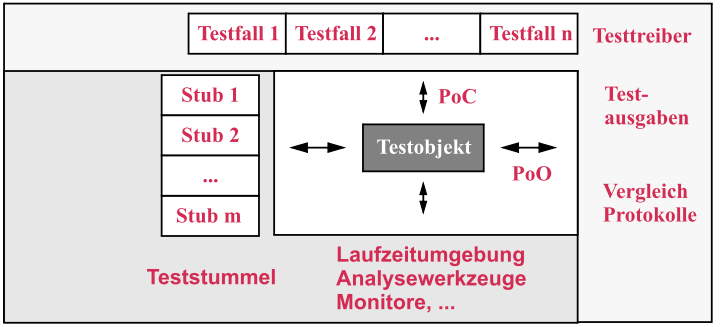
\includegraphics[width=0.85\textwidth]{4_1_1}
\end{figure}

\begin{itemize}
	\item \textbf{Point of Control (PoC): }
	\begin{itemize}
		\item Schnittstelle, über die Testobjekt mit Testdaten versorgt wird
	\end{itemize}
	\item \textbf{Point of Observation (PoO)}
	\begin{itemize}
		\item Schnittstelle, über die Reaktionen/Ausgaben des Testobjekts beobachtet werden
	\end{itemize}
\end{itemize}

\paragraph{Wie wird getestet - Arten von Testverfahren:}

\begin{itemize}
	\item \textbf{Funktionstest}(black box test): die interne Struktur der Komponente wird nicht betrachtet; getestet wird Ein-/Ausgabeverhalten gegen Spezifikation (informell oder formal);
	\item \textbf{Strukturtest}  (white box test): interne Struktur der Komponente wird zur Testplanung und -Überwachung herangezogen:
	\begin{itemize}
		\item Kontrollflussgraph
		\item Datenflussgraph
		\item Automaten
	\end{itemize}
	\item \textbf{Diversifikationstest} Verhalten einer Komponentenversion wird mit Verhalten anderer Komponentenversionen verglichen
\end{itemize}

\paragraph{Diversifikationstestverfahren:}

Das Verhalten verschiedener Varianten eines Programms wird verglichen
\begin{itemize}
	\item \textbf{Mutationstestverfahren}: ein Programm wird absichtlich durch Transformationen verändert und damit in aller Regel mit Fehlern versehen
	\begin{itemize}
		\item Einbau von Fehlern lässt sich (mehr oder weniger) automatisieren
		\item eingebaute Fehler entsprechen oft nicht tatsächlich gemachten Fehlern
		\item eingebaute Fehler stören Suche nach echten Fehlern
	\end{itemize}
	\item \textbf{N-Versionen-Programmierung}: verschiedene Versionen eines Programms werden völlig unabhängig voneinander entwickelt
	\begin{itemize}
		\item sehr aufwändig, da man mehrere Entwicklerteams braucht (und gegebenfalls sogar Hardware mehrfach beschaffen muß)
		\item Fehler der verschiedenen Teams nicht unabhängig voneinander (z.B. haben alle Versionen dieselben Anforderungsdefinitionsfehlern)
	\end{itemize}
\end{itemize}

\paragraph{Mutationstestverfahren:}

\textbf{Erzeugung von Mutationen durch:} \\
Vertauschen von Anweisungsfolgen, Umdrehen von Kontrollflussbedingungen, Löschen von Zuweisungen, Ändern von Konstanten, …
\\
\\
\textbf{Zielsetzungen:}
\begin{itemize}
	\item I\textbf{dentifikation fehlender Testfälle}: für jeden Mutanten sollte mindestens ein Testfall existieren, der Original und Mutant unterscheiden kann
	\item \textbf{Eliminination nutzloser Testfälle}: Gruppe von Testfällen verhält sich bezüglich der Erkennung von Mutanten völlig gleich
	\item Schätzung der Restfehlermenge RF: RF \~ GF*(M/GM-1) \\
	\textbf{Annahme:}  GF/F ~ GM/M (Korrelation gilt allenfalls für bestimmte Fehler) \\
	mit:
	\begin{itemize}
		\item GM = Anzahl gefundener eingebauter Fehler (Mutationen)
		\item M  = Gesamtzahl absichtlich eingebauter Fehler
		\item GF  = Anzahl gefundener echter Fehler
		\item F = Gesamtzahl echter Fehler = GF + RF
	\end{itemize}
\end{itemize}

\paragraph{N-Versionen-Programmierung (Back-to-Back-Testing):}

\textbf{Zielsetzungen:}
\begin{itemize}
	\item eine Version kann als Orakel für die Korrektheit der Ausgaben einer anderen Version herangezogen werden (geht ab 2 Versionen)
	\item Robustheit der ausgelieferten Software kann erhöht werden durch gleichzeitige Berechnung eines benötigten Ergebnisses durch mehrere Versionen einer Software
	\item Liefern verschiedene Versionen unterschiedliche Ergebnisse, so wird Mehrheitsentscheidung verwendet (geht ab 3 Versionen)
\end{itemize}
\textbf{Probleme:}
\begin{itemize}
	\item N Versionen enthalten mehr Fehler als eine Version: falsche Versionen können richtige überstimmen oder gemeinsame Ressourcen blockieren
	\item Fehler verschiedener Versionen sind nicht immer unabhängig voneinander: Fehler aus der Anforderungsdefinition oder typische Programmiersprachenfehler oder falsche Algorithmen können alle Versionen enthalten
\end{itemize}

\paragraph{Exkurs zur Berechnung von Ausfallwahrscheinlichkeiten:}

Für die Berechnung der Ausfallwahrscheinlichkeit eines (Software-)Systems wird der innere Aufbau des Systems wie folgt als ein gerichteter (Kontrollfluss-)Graph bzw. Abhängigkeitsgraph $S=(N,E,n_{start},n_{final})$ dargestellt:
\begin{itemize}
	\item die Knoten N sind die \textbf{Komponenten}, aus denen das System besteht
	\item die Kanten E beschreiben \textbf{Berechnungsabhängigkeiten} bzw. -pfade zwischen den Komponenten des Systems
	\item eine zusätzlich gegebene Funktion A: N ->[0..1] legt für jede Komponente n deren \textbf{Ausfallwahrscheinlichkeit} A(n) fest, die unabhängig von den Ausfallwahrscheinlichkeiten anderer Komponenten sein soll
\end{itemize}
Ein solches System gilt im einfachsten Fall als genau dann \textbf{ausgefallen}, sobald es keinen Pfad von $n_{start}$ nach $n_{final}$ gibt, af dem keine Komponente ausgefallen ist.

\paragraph{Einfache Rechenregeln für System-Ausfallwahrscheinlichkeit:}

Eine \textbf{''Parallelschaltung''} zweier unabhängiger Komponenten $n_{1}$  und $n_{2}$  fällt dann aus, wenn beide Komponenten ausfallen. Das Bild rechts 
zeigt die Ersetzung der Parallelschaltung der beiden Komponenten $n_{1}$  und $n_{2}$  durch eine Komponente n mit gleicher Ausfallwahrscheinlichkeit.
\\
\\
Eine \textbf{''Reihenschaltung''} zweier unabhängiger Komponenten $n_{1}$  und $n_{2}$  ist dann nicht ausgefallen, wenn beide Komponenten nicht ausgefallen sind. Das Bild rechts zeigt die Ersetzung der Reihenschaltung von $n_{1}$  und $n_{2}$  durch eine Komponente n mit gleicher Ausfallwahrscheinlichkeit.

\paragraph{Rekursive Rechenregel für System-Ausfallwahrscheinlichkeit}

Die Berechnung der Ausfallwahrscheinlichkeit eines Systems S lässt sich bei Fokus auf den Status einer bestimmten Komponente n in zwei Fälle zerlegen:
\begin{enumerate}
	\item Berechnung der Ausfallwahrscheinlichkeit von S unter der Annahme, dass die \textbf{Komponente n ausgefallen} ist $=A(S)_{n ist ausgefallen}$; n ist ausgefallen  ; dabei sei A(n) die Wahrscheinlichkeit, dass Komponente n ausgefallen ist.
	\item Berechnung der Ausfallwahrscheinlichkeit von S unter der Annahme, dass die \textbf{Komponente n nicht ausgefallen} ist $=A(S)_{n ist nicht ausgefallen}$; dabei sei 1-A(n) die Wahrscheinlichkeit, dass Komponente n nicht ausgefallen ist.
\end{enumerate}
Damit ergibt sich 
\begin{equation}
	A(S)=A(n) \cdot A(s)_{n ist ausgefallen} + (a-A(n)) \cdot A(S)_{n ist nicht ausgefallen}
\end{equation}
Als Komponente n für die Fallunterscheidung wählt man geschickterweise eine Komponente, die ansonsten die vollständige Dekomposition des betrachteten Graphen in  einfach zu behandelnde Serien- und Parallelschaltungen verhindert. Die Berechnung erfolgt durch die Berechnung der Ausfallwahrscheinlichkeiten zweier ''Ersatzschaltbilder'':
\begin{enumerate}
	\item $A(S)_{n ist ausgefallen}=A(S1)$
	\item $A(S)_{n ist nicht ausgefallen}=A(S2)$
\end{enumerate}

\begin{figure}[h]
	\centering
	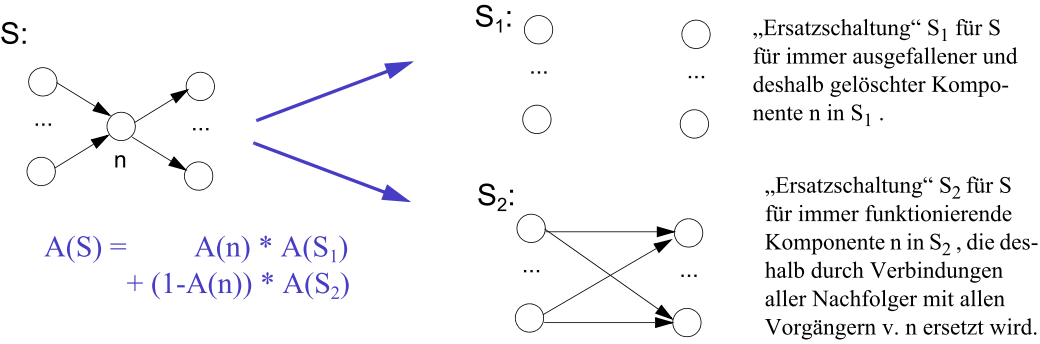
\includegraphics[width=0.85\textwidth]{4_1_2}
\end{figure}

In einigen Fällen muss man auch Komponenten behandeln, die nur dann ''funktionieren'', wenn alle ihre Eingänge korrekte Eingaben erhalten (und damit alle ihre Vorgängerkomponenten nicht ausgefallen sind). Wenn bei einer solchen Komponente eine Vorgängerkomponente ausfällt, fällt die Komponente selbst auch aus.

\paragraph{Alternative Berechnung der Ausfallwahrscheinlichkeit von n Versionen:}

n parallel geschaltete Versionen enthalten in etwa n-mal so viele Fehler wie eine Version, aber falls Wahrscheinlichkeit A für fehlerhafte Arbeitsweise einer Version v unabhängig vom Ausfall anderer Versionen ist, dann gilt:
\begin{itemize}
	\item Richtiges Ergebnis werde berechnet, solange höchstens $\lfloor(n+1)/2\rfloor$ Versionen fehlerhaft arbeiten (n ist sinnvoller Weise ungerade Zahl; ansonsten abrunden)
	\item Wahrscheinlichkeit für gleichzeitigen Ausfall von k unabhängigen Versionen: \\
	$\left(
	\begin{array}{c}
	n \\
	k
	\end{array} x A^k x (1-A)^{(n-k)} =
	\frac{\prod_{i=n-k+1}^{v}i}{\prod_{i=1}^{k}i} x A^k x (1-A)^{(n-k)}
	\right)$
	\item Wahrscheinlichkeit für \textbf{Ausfall des Gesamtsystems} mit n Versionen (bei n=3: Wahrscheinlichkeit für Ausfall von 2 oder 3 Versionen): \\
	$\sum_{\lfloor(n+1)/2\rfloor}^{n\left(
		\begin{array}{c}
		n \\
		k
		\end{array} \right) x A^k x (1-A)^{(n-k)}}$ 
\end{itemize}


\begin{figure}[h]
	\centering
	\caption{Der Testprozess als Bestandteil des Softwareentwicklungsprozesses}
	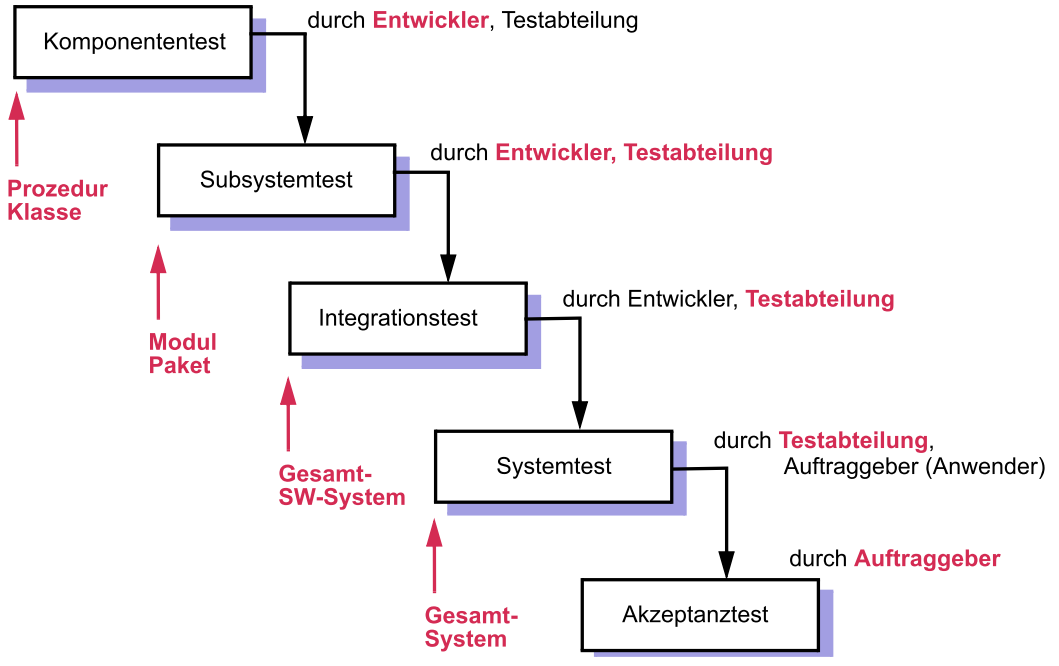
\includegraphics[width=0.85\textwidth]{4_1_3}
\end{figure}


\begin{figure}[h]
	\centering
	\caption{Der Testprozess als Bestandteil des Softwareentwicklungsprozesses}
	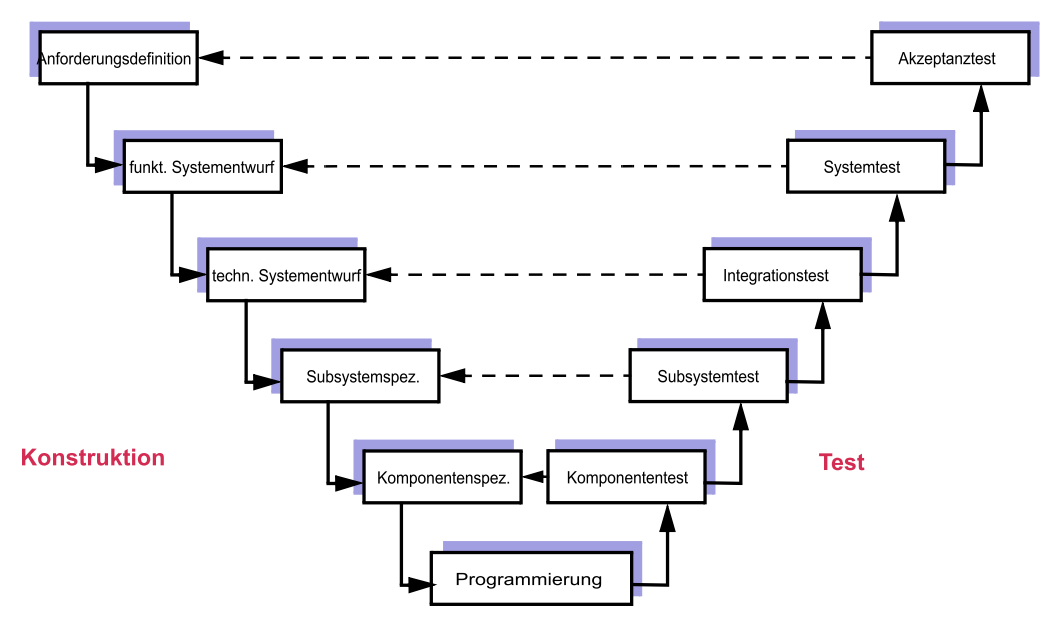
\includegraphics[width=0.85\textwidth]{4_1_4}
\end{figure}

\paragraph{Komponententest (Unit-Test) und Subsystemtest:}

\begin{itemize}
	\item jeweils ein \textbf{einzelner Softwarebaustein} wird überprüft, isoliert von anderen Softwarebausteinen des Systems
	\item die betrachtete Komponente (Unit) kann eine Klasse, Paket (Modul) sein
	\item \textbf{Subsystemtest} kann als Test einer besonders großen Komponente aufgefasst werden
	\item getestet wird gegen die Spezifikation der Schnittstelle der Komponente, dabei betrachtet werden funktionales Verhalten, Robustheit, Effizienz, ...
	\item Testziele sind das Aufdecken von Berechnungsfehlern, Kontrollflussfehlern, ...
	\item getestet wird in jedem Fall die Komponente für sich mit
	\begin{itemize}
		\item \textbf{Teststummel} (Platzhalter, Dummies, Stubs) für benötigte Dienste anderer Komponenten
		\item \textbf{Testtreibern}(Driver) für den (automatisierten) Test der Schnittstelle (für Eingabe von Parametern, Ausgabe von Parametern, ... )
	\end{itemize}
\end{itemize}

\paragraph{Integrationtest:}

\begin{itemize}
	\item das gesamte Software-System (oder ein abgeschlossenes Teilsystem) wird getestet; Schwerpunkt liegt dabei auf Test des \textbf{Zusammenspiels} der Einzelkomponenten
	\item normalerweise wird vorausgesetzt, dass Einzelkomponenten vorab bereits getestet wurden
	\item auch hier müssen wieder \textbf{Testtreiber} (Testwerkzeuge) verwendet werden, die die zu testende Komponente aufrufen bzw. steuern
	\item auf \textbf{Teststummel} kann meist verzichtet werden, da alle benötigten Teilsysteme zusammen getestet werden
	\item \textbf{Testziel} ist vor allem das Aufdecken von \textbf{Schnittstellenfehlern} und insbesondere Fehler beim Austausch von Daten
\end{itemize}

\paragraph{Gängige Integrationsteststrategien:}
\begin{itemize}
	\item \textbf{''Big Bang''-Strategie}: alle Teile sofort integrieren und nur als Gesamtheit testen
	\begin{itemize}
		\item Lokalisierung von Fehlern schwierig
		\item Arbeitsteilung kaum möglich
		\item Testen beginnt zu spät
	\end{itemize}
	\item \textbf{''Top-down''-Testverfahren:} zuerst A mit Dummies für B,C und D; dann B mit Dummies für E und F,...
	\begin{itemize}
		\item Erstellung ''vernünftiger'' Dummies schwierig
		\item Test der Basisschicht sehr spät
	\end{itemize}
	\item \textbf{''Bottom-Up''-Testverfahren:} zuerst E,F,G und H mit Testtreibern, die Einbindung in B,C und D simulieren, dann B,C und D mit Testtreiber...
	\begin{itemize}
		\item Test des Gesamtverhaltens des Systems gegen Lastenheft erst am Ende
		\item Designfehler und Effizienzprobleme werden oft erst spät entdeckt
	\end{itemize}
	\item \textbf{Ad-Hoc-Integration:} die Komponenten werden in der (zufälligen) Reihenfolge ihrer Fertigstellung integriert und getestet
	\item \textbf{Backbone-Integration (Inkrementelle Vorgehensweise):} zunächst wird Grundgerüst erstellt, weitere Komponenten werden stückweise hinzugefügt
	\begin{itemize}
		\item wie erstellt und testet man Grundgerüst (z.B. Top-Down-Testen)
		\item Hinzufügen von Komponenten kann bisherige Testergebnisse entwerten
	\end{itemize}
	\item \textbf{Regressionstest (für inkrementelle Vorgehensweise):} da Änderungen neue Fehlerzustände in bereits getesteten Funktionen verursachen (oder bislang maskierte Fehlerzustände sichtbar machen) können werden
	\begin{itemize}
		\item möglichst viele Tests automatisiert
		\item bei jeder Änderung werden alle vorhandenen Tests durchgeführt
		\item neue Testergebnisse mit alten Testergebnissen verglichen
	\end{itemize}
\end{itemize}


\begin{figure}[h]
	\centering
	\caption{Gängige Integrationsteststrategien}
	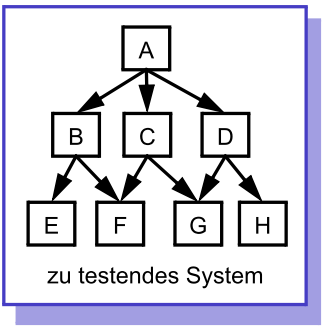
\includegraphics[width=0.3\textwidth]{4_1_5}
\end{figure}

\paragraph{Systemtest - grundsätzliche Vorgehensweise:}
\begin{itemize}
	\item Nach abgeschlossenem Integrationstest und vor dem Abnahmetest erfolgt der Systemtest beim Softwareentwickler durch Kunden $\alpha-Test$
	\item Variante: Systemtests bei ausgewählten Pilotkunden vor Ort $\beta-Test$
	\item Systemtest überprüft aus der \textbf{Sicht des Kunden}, ob das Gesamtprodukt die an es gestellten Anforderungen erfüllt (nicht mehr aus Sicht des Entwicklers)
	\item anstelle von Testtreibern und Teststummeln kommen nun soweit möglich immer die realen (Hardware-)Komponenten zum Einsatz
	\item Systemtest sollte nicht beim Kunden in der Produktionsumgebung stattfinden, sondern in möglichst realitätsnaher Testumgebung durchgeführt werden
	\item beim Test sollten die \textbf{tatsächlichen Geschäftsprozesse} beim Kunden berücksichtigt werden, in das getestete System eingebettet wird
	\item dabei durchgeführt werden: Volumen- bzw. Lasttests (große Datenmengen), Stresstests (Überlastung), Test auf Sicherheit, Stabilität, Robustheit, ...
\end{itemize}

\paragraph{Systemtest - nichtfunktionale Anforderungen:}
\begin{itemize}
	\item  \textbf{Lasttest}: Messung des Systemverhaltens bei steigender Systemlast
	\item \textbf{Performanztest}: Messung der Verarbeitungsgeschwindigkeit unter bestimmten Randbedingungen
	\item \textbf{Kompatibilität}: Verträglichkeit mit vorhandenen anderen Systemen, korrekter Import und Export externer Datenbestände, ...
	\item \textbf{Benutzungsfreundlichkeit}: übersichtliche Oberfläche, verständliche Fehlermeldungen, Hilfetexte, ... - für die jeweilige Benutzergruppe
	\item \textbf{Benutzerdokumentation}: Vollständigkeit, Verständlichkeit, ...
	\item \textbf{Änderbarkeit, Wartbarkeit}: modulare Systemstruktur, verständliche Entwicklerdokumentation, ...
	\item ...
\end{itemize}

\paragraph{Akzeptanztest (Abnahmetest):}
\begin{itemize}
	\item Es handelt sich um eine \textbf{spezielle Form des Systemtests}
	\begin{itemize}
		\item der Kunde ist mit einbezogen bzw. führt den Test durch
		\item der Test findet beim Kunden, aber in Testumgebung statt (Test in Produktionsumgebung zu gefährlich)
	\end{itemize}
	\item auf Basis des Abnahmetests entscheidet Kunde, ob das bestellte Softwaresystem \textbf{mangelfrei} ist und die im Lastenheft festgelegten Anforderungen erfüllt
	\item die durchgeführten Testfälle sollten bereits im \textbf{Vertrag} mit dem Kunden spezifiziert sein
	\item im Rahmen des Abnahmetests wird geprüft, ob System von allen relevanten Anwendergruppen \textbf{akzeptiert} wird
	\item im Rahmen von sogenannten \textbf{Feldtests} wird darüber hinaus ggf. das System in verschiedenen Produktionsumgebungen getestet
\end{itemize}

\paragraph{Testen, testen, ... - wann ist Schluss damit?}
\begin{itemize}
	\item \textbf{nie} - nach jeder Programmänderung wird eine große Anzahl von Testfällen automatisch ausgeführt (siehe Regressionstest)
	\item Testbudget verbraucht bzw. Auslieferungszeitpunkt für Software erreicht (der Kunde testet unfreiwillig weiter ... )
	\item je Testfall (Zeiteinheit) gefundene Fehlerzahl sinkt unter gegebene Grenze (in der Hoffnung, dass die Anzahl der im Programm verbliebenen Fehler mit der Anzahl der pro Zeiteinheit gefundenen Fehler korreliert)
	\item n\% absichtlich von einer Gruppe implantierter Fehler (seeded bugs) wurden von Testgruppe gefunden (siehe auch Mutationstestverfahren)
	\item gemäß systematischen Verfahren werden aus allen möglichen Eingabedatenkombinationen typische Repräsentanten ausgewählt und genau diese getestet
	\item Testfälle decken hinreichend viele (relevante) Programmdurchläufe ab
\end{itemize}

\paragraph{Die sieben Grundsätze des Testens nach [SL19]:}
\begin{enumerate}
	\item Testen zeigt die Anwesenheit von Fehlern (und nie die Abwesenheit)
	\item Vollständiges Testen ist nicht möglich
	\item Mit dem Testen frühzeitig beginnen
	\item Häufung von Fehlern (in bestimmten Programmteilen)
	\item Zunehmende Testresistenz (gegen existierende Tests)
	\item Testen ist abhängig vom Umfeld
	\item \textbf{Trugschluss}: Keine Fehler bedeutet ein brauchbares System
\end{enumerate}

\subsection{Laufzeit- und Speicherplatzverbrauchsmessungen}
Gemeinsame Eigenschaft aller hier vorgestellten Werkzeuge/Verfahren ist:
\begin{itemize}
	\item Objektcode für untersuchte Software wird vor Ausführung ''instrumentiert'' (um zusätzliche Anweisungen ergänzt)
	\item zusätzliche Anweisungen erzeugen während der Ausführung statistische Daten über Laufzeitverhalten, Speicherplatzverbrauch, ...
\end{itemize}


\begin{figure}[h]
	\centering
	\caption{Laufzeit- und Speicherplatzverbrauchsmessungenn}
	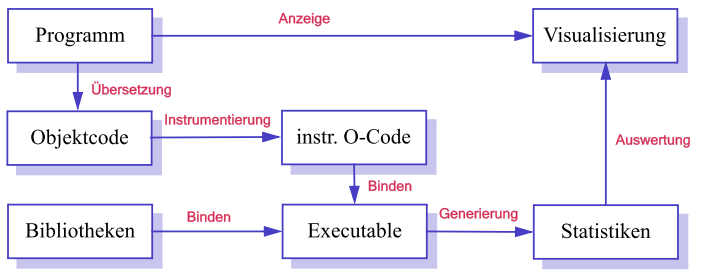
\includegraphics[width=0.85\textwidth]{4_2}
\end{figure}

\paragraph{Untersuchung des Laufzeitverhaltens eines Programms:}
\begin{itemize}
	\item wie oft wird jede Operation aufgerufen (oder Quellcodezeile durchlaufen)
	\item welche Operation ruft wie oft welche andere Operation (\textbf{descendants}) auf oder von welchen Operationen (\textbf{callers}) wird ein Programm wie oft gerufen
	\item wieviel Prozent der Gesamtlaufzeit wird mit Ausführung einer bestimmten Operation verbracht (ggf. aufgeteilt nach callers und descendants)
	\item ...
\end{itemize}

\paragraph{Nutzen der ermittelten Daten:}
\begin{itemize}
	\item  Operationen, die am meisten Laufzeit in Anspruch nehmen, können leicht identifiziert (und optimiert) werden
	\item tatsächliche Aufrufabhängigkeiten werden sofort sichtbar
	\item ...
\end{itemize}

\paragraph{Untersuchung des Speicherplatzverhaltens eines Programms:}
\begin{itemize}
	\item welche Operationen fordern wieviel Speicherplatz an (geben ihn frei)
	\item wo wird Freigabe von Speicherplatz vermutlich bzw. bestimmt vergessen (memory leak = Speicherloch):
	\begin{itemize}
		\item bestimmt vergessen: Objekt lebt noch, kann aber nicht mehr erreicht werden (Garbage Collector von Java würde es entsorgen)
		\item vermutlich vergessen: Objekt lebt noch und ist erreichbar, wird aber nicht mehr benutzt (Garbage Collector von Java kann es nicht freigeben)
	\end{itemize}
	\item wo wird auf bereits freigegebenen Speicherplatz zugegriffen (nur für C++) bzw. wo wird Speicherplatz mehrfach freigegeben (nur für C++)
	\item wo wird auf nicht initialisierten Speicherplatz zugegriffen; anders als bei der statischen Programmanalyse wird für jede Feldkomponente (Speicherzelle) getrennt Buch darüber geführt 
	\item wo finden Zugriffe jenseits der Grenzen von Arrays statt (Laufzeitfehler in guter Programmiersprache)
\end{itemize}

\subsection{Funktionsorientierte Testverfahren (Blackbox)}

Sie testen Implementierung gegen ihre Spezifikation und lassen die interne Programmstruktur unberücksichtigt (Programm wird als ''Black-Box'' behandelt):
\begin{itemize}
	\item für \textbf{Abnahmetest} ohne Kenntnis des Quellcodes geeignet
	\item setzt (eigentlich) vollständige und widerspruchsfreie \textbf{Spezifikation} voraus (zur Auswahl von Testdaten und Interpretation von Testergebnissen)
	\item \textbf{repräsentative Eingabewerte} müssen ausgewählt werden (man kann im allgemeinen nicht alle Eingabekombinationen testen)
	\item man braucht ''Orakel'' für Überprüfung der Korrektheit der Ausgaben (braucht man allerdings bei allen Testverfahren)
\end{itemize}

Eingaben -> Testobjekt -> Ausgaben -> Orakel -> Ausgabe ok?

\paragraph{Kriterien für die Auswahl von Testdaten:}

An der Spezifikation orientierte \textbf{Äquivalenzklassenbildung}, so dass für alle Werte einer Äquivalenzklasse (Eingabewertklasse) sich das Softwareprodukt ''gleich'' verhält:
\begin{itemize}
	\item Unterteilung in Klassen von Eingabewerten, für die das Programm sich laut Spezifikation gleich verhalten muss
	\item Alle Klassen von Eingabewerten zusammen müssen den ganzen möglichen Eingabewertebereich des betrachteten Programms abdecken
	\item Aus jeder Äquivalenzklasse wird mindestens ein repräsentativer Wert getestet
	\item Unterteilung in gültige und ungültige Eingabewerte (fehlerhafte Eingaben, ... ) wird durchgeführt und später bei der Auswahl von Testwerten berücksichtigt
	\item Oft gibt es auch eine gesonderte Betrachtung von Äquivalenzklassen für besonders ''große'' oder besonders ''kleine'' gültige Eingaben (Lasttest)
	\item Hier nicht mit betrachtet wird die Problematik der Suche nach Eingabewerteklassen, die zu bestimmten (Klassen von) Ausgabewerten führen 
\end{itemize}

\paragraph{Regeln für die Festlegung von Eingabewerteklassen:}
\begin{itemize}
	\item für geordnete Wertebereiche:
	\begin{itemize}
		\item $]uv..ov[$ ist ein offenes Intervall aller Werte zwischen $uv$ und $ov$ ($uv$ und $ov$ selbst gehören nicht dazu)
		\item $[uv..ov]$ ist ein geschlossenes Intervall aller Werte zwischen $uv$ und $ov$ ($uv$ und $ov$ selbst gehören dazu)
		\item Mischformen $]uv...ov]$ und $[uv..ov[$ sind natürlich erlaubt
	\end{itemize}
	\item für ganze Zahlen (Integer):
	\begin{itemize}
		\item $[MinInt..ov]$ für Intervalle mit kleinster darstellbarer Integer-Zahl
		\item $[uv..MaxInt]$ für Intervalle mit größter darstellbarer Integer-Zahl
		\item offene Intervallgrenzen sind natürlich erlaubt
	\end{itemize}
	\item für reelle Zahlen (Float) mit Voraussetzung kleinste/größte Zahl nicht darstellbar:
	\begin{itemize}
		\item $]-\infty..ov]$ oder $]-\infty..ov[$ für nach unten offene Intervalle
		\item $[uv..\infty[$ oder $]uv..\infty$ für nach oben offene Intervalle
		\item alle Mischformen von Intervallen mit festen unteren und oberen Grenzen
	\end{itemize}
	\item für Zeichenketten (String):
	\begin{itemize}
		\item Definition über reguläre Ausdrücke oder Grammatiken
		\item Aufzählung konkreter Werte (siehe nächster Punkt)
	\end{itemize}
	\item für beliebige Wertebereiche:
	\begin{itemize}
		\item {v1 v2 v3 ... vn} für Auswahl von genau n verschiedenen Werten
	\end{itemize}
	\item für zusammengesetzte Wertebereiche:
	\begin{itemize}
		\item Anwendung der obigen Prinzipien auf die einzelnen Wertebereiche
		\item ggf. braucht man noch zusätzliche Einschränkungen (Constraints), die nur bestimmte Wertekombinationen für die Teilkomponenten zulassen
	\end{itemize}
	\item Eingabewerteklassen, die aus genau einem Wert bestehen:
	\begin{itemize}
		\item [v] es ist aber auch die Repräsentation {v} oder v üblich
	\end{itemize}
\end{itemize}

\paragraph{Auswahl von Testdaten aus Eingabewerteklassen:}

\begin{itemize}
	\item aus jeder Eingabewerteklasse wird mindestens ein Wert ausgewählt (Fehler- und Lasttestklassen werden später gesondert behandelt) 
	\item gewählt werden meist nicht nur die Grenzen selbst, sondern auch die um eins größeren und kleineren Werte (siehe ISTQB-Prüfung; im Folgenden werden aus Platzgründen bei den Beispielen aber nur Grenzwerte selbst ausgewählt)
	\item als Intervalle dargestellte Eingabewerteklassen werden oft durch die so genannte \textbf{Grenzwertanalyse} nochmal in Unterklassen/Teilintervalle zerlegt:
	\begin{itemize}
		\item $]uv..ov[$ wird zerlegt $[inc(uv)] ]inc(uv)..dec(ov)[ [dec(ov)]$
		\item $[uv..ov]$ wird zerlegt in $[uv] ]uv..ov[ [ov]$
		\item ...
		\item $inc(uv)$ liefert den nächstgrößeren Wert zu uv
		\item $dec(ov)$ liefert den nächstkleineren Wert zu ov
		\item Achtung: bei Float muss für inc und dec die gewünschte Genauigkeit festgelegt werden, mit der aufeinanderfolgende Werte gewählt werden
	\end{itemize}
\end{itemize}

\paragraph{Zusätzliche Wahl von Testdaten durch Grenzwertanalyse:}

Bilden Eingabewerteklassen einen Bereich (Intervall), so selektiert die Grenzwertanalyse also immer Werte um die Bereichsgrenzen herum:
\begin{itemize}
	\item gewählt werden meist nicht nur die Grenzen selbst, sondern auch die um eins größeren und kleineren Werte (im Folgenden aus Platzgründen weggelassen)
	\item Idee dabei: oft werden Schleifen über Intervallen gebildet, die genau für die Grenzfälle falsch programmiert sind
\end{itemize}

\paragraph{Auswahl von Testeingaben für countVowels (mit Zeichenketten!):}
s = sentence
\begin{itemize}
	\item Klasse 1: s endet nicht mit einem Punkt (oh je, das geht schief)
	\item Klasse 2: s endet mit einem Punkt und enthält keine Vokale
	\begin{itemize}
		\item s besteht nur aus einem Punkt
		\item s besteht aus einem Konsonanten gefolgt von einem Punkt
		\item s enthält sonstige Sonderzeichen
	\end{itemize}
	\item Klasse 3: s endet mit einem Punkt und enthält einen Vokal:
	\begin{itemize}
		\item 3a: s enthält ein a, e, i, o, u
		\item 3b: s enthält ein A, E, I, O, U (oh je, dieser Fall wurde auch vergessen)
	\end{itemize}
	\item Klasse 4: s enthält mehrere Vokale:
	\begin{itemize}
		\item 4a: mehrere gleiche Vokale
		\item 4b: mehrere verschiedene Vokale
	\end{itemize}
	\item Klasse 5: Eingabe ist sehr lang und enthält ganz viele Vokale
\end{itemize}

\paragraph{Weitere Regeln für die Bildung von Äquivalenzklassen bei Intervallen:}
\begin{itemize}
	\item aus Äquivalenzklassen, die (geschlossene) Intervalle sind, werden jeweils die beiden Grenzwerte und ein weiterer Wert (z.B. aus der Mitte des Intervalls) ausgewählt (ohne platzraubenden Zwischenschritt der Zerlegung in drei Teilintervalle)
	\item einelementige Äquivalenzklasse und Wert aus dieser Äquivalenzklasse werden nicht unterschieden, also statt [v] schreiben wir gleich v
	\item reguläre Ausdrücke werden zur Definition v. String-Äquivalenzklassen eingesetzt
\end{itemize}

\paragraph{Grafische Darstellung von Äquivalenzklassen als Klassifikationsbaum:}

\begin{figure}[h]
	\centering
	\caption{Grafische Darstellung von Äquivalenzklassen als Klassifikationsbaum}
	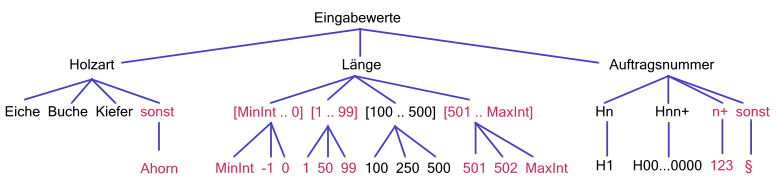
\includegraphics[width=0.85\textwidth]{4_3}
	
\end{figure}
\begin{itemize}
	\item zunächst wird ''Eingabewerte'' in alle Eingabeparameter des Programms zerlegt
	\item zusammengesetzte Eingabeparameter werden weiter zerlegt
	\item schließlich wird der Wertebereich eines atomaren Eingabeparameters betrachtet
	\item der Wertebereich wird in Äquivalenzklassen „ähnlicher“ Werte zerlegt
	\item dabei werden auch nicht erlaubte Eingabewerte (Fehlerklassen) betrachtet
	\item ebenso werden ''extreme'' erlaubte Werte (Lasttestklassen) betrachtet
	\item aus jedem Wertebereich werden Repräsentanten für den Test ausgewählt
\end{itemize}

\paragraph{Unvollständige/fehlerhafte Auswahl von Eingabewertekombinationen:}

\begin{figure}[h]
	\centering
	\caption{Unvollständige/fehlerhafte Auswahl von Eingabewertekombinationen}
	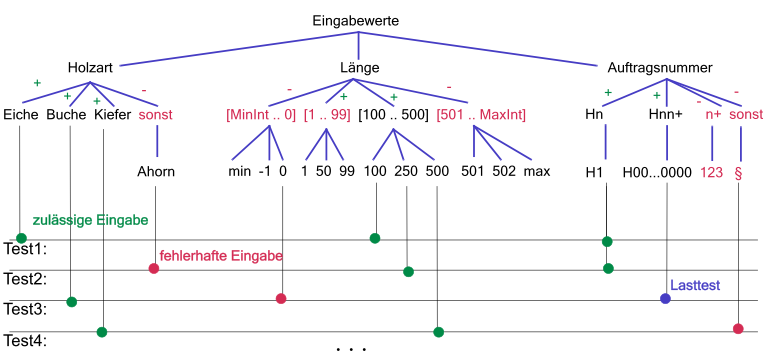
\includegraphics[width=0.85\textwidth]{4_3_1}
\end{figure}

\textbf{Problem:} trotz Bildung von Äquivalenzklassen bleiben (zu) viele mögliche Eingabewertekombinationen (im Beispiel sind 4 * 12 * 4 verschiedene Testläufe möglich).

\paragraph{Heuristiken für die Reduktion möglicher Eingabewertekombinationen:}

\begin{itemize}
	\item aus jeder \textbf{Äquivalenzklasse} wird mindestens einmal ein Wert ausgewählt; es gibt also jeweils mindestens einen Testfall, in dem ein Eingabewert der Äquivalenzklasse verwendet wird (bei Grenzwertanalyse werden drei Werte ausgewählt)
	\item bei \textbf{abhängigen Eingabeparametern} müssen Testfälle für \textbf{alle Kombinationen} ihrer jeweiligen ''normalen'' Äquivalenzklassen aufgestellt werden; Parameter sind abhängig, wenn sie gemeinsam das Verhalten des Programms steuern (und deshalb nicht unabhängig voneinander betrachtet werden können)
	\item der ausgewählte \textbf{Wert} einer \textbf{Fehleräquivalenzklasse} wird in genau einem Testfall verwendet (Fehleräquivalenzklassen sind solche Äquivalenzklassen, die unzulässige Eingabewerte zusammenfassen)
	\item der ausgewählte \textbf{Wert} einer \textbf{Lasttestklasse} wird ebenfalls genau einmal in einem Testfall verwendet  (Lasttestklassen sind solche Äquivalenzklassen, die besonders ''große/lange/...'' zulässige/gültige Eingabewerte zusammenfassen)
	\item hat man mehrere Eingabeparameter, wird \textbf{höchstens einer} mit einem Wert aus einer Fehler- oder Lasttestklasse belegt (verhindert Verdeckung von Fehlern)
\end{itemize}

\paragraph{''Normierter'' Aufbau von Klassifikationsbäumen für Übung/Klausur:}


\begin{enumerate}
	\item Ebene: alle Parameter(-namen) der betrachteten Funktion
	\item Ebene: die Typen bzw. Wertebereiche der Parameter
	\item Ebene: die Zerlegung der Wertebereiche in
	\begin{itemize}
		\item Äquivalenzklassen für erlaubte Werte (mit ''+'' markiert)
		\item Fehleräquivalenzklassen (mit ''-'' markiert)
	\end{itemize}
	\item Ebene:  weitere Zerlegung der Wertebereiche mit Grenzwertanalyseverfahren
	\item Ebene:  konkrete Repräsentanten (Werte) der jeweiligen Äquivalenzklassen
\end{enumerate}

\paragraph{Paarweiser Testansatz (Pairwise Testing):}

Die Praxis zeigt, dass ca. 80\% aller von bestimmten Parameterwertkombinationen ausgelösten Softwarefehler bereits durch Wahl bestimmter Paarkombinationen beobachtet werden können. Also werden beim ''paarweisen'' Testen einer Funktion mit n Parametern nicht alle möglichen Kombinationen überprüft, sondern nur alle paarweisen Kombinationen.

\paragraph{Bewertung der funktionalen Äquivalenzklassenbildung:}

\begin{itemize}
	\item Güte des Verfahrens hängt stark von \textbf{Güte der Spezifikation} ab (Aussagen über erwartete/zulässige Eingabewerte und Ergebnisse)
	\item Verwaltung von Äquivalenzklassen und Auswahl von Testfällen kann durch \textbf{Werkzeugunterstützung} vereinfacht werden
	\item \textbf{ausführbare Modelle} (z.B. in UML erstellt) können bei der Auswahl von Äquivalenzklassen, Testfällen helfen (und als Orakel verwendet werden)
	\item Test von Benutzeroberflächen, zeitlichen Beschränkungen, Speicherplatzbeschränkungen etc. (\textbf{nichtfunktionale Anforderungen}) wird kaum unterstützt
	\item mindestens \textbf{einmalige Ausführung} jeder Programmzeile wird nicht garantiert
	\item Test \textbf{zustandsbasierter Software} (Ausgabeverhalten hängt nicht nur von Eingabe, sondern auch von internem Zustand ab) geht so nicht
	\begin{itemize}
		\item später Spezifikation und Testplanung mit Hilfe von Automaten/Statecharts
		\item Grenzfall zwischen funktionalem und strukturorientiertem Softwaretest
	\end{itemize}
\end{itemize}

\paragraph{Weitere Black-Box-Testverfahren}
\begin{itemize}
	\item \textbf{Erfahrungsbasierte Testverfahren:}
	\begin{itemize}
		\item \textbf{Intuitives Testen (Error Guessing)}: ein Testansatz, bei dem Testfälle auf Basis des Wissens der Tester über frühere Fehler oder allgemeines Wissen über Fehlerwirkungen (irgendwie) abgeleitet werden
		\item \textbf{Exploratives Testen}: ein Testansatz bei dem die Tester, basierend auf ihrem Wissen, der Erkundung des Testobjekts und dem Ergebnis früherer Tests, dynamisch neue Tests entwickeln
		\item \textbf{Checklistenbasiertes Testen}: ein Testansatz bei dem erfahrene Tester eine Liste von Kontrollpunkten (Checkliste) bzw. Regeln oder Kriterien (für das Testobjekt) zur Steuerung des Testprozesses nutzen
	\end{itemize}
	\item \textbf{Zufallstest}: wählt aus Menge der möglichen Werte eines Eingabedatums zufällig Repräsentanten aus (ggf. gemäß bekannter statistischer Verteilung)
	\begin{itemize}
		\item zur Ergänzung gut geeignet, generiert oft ''unerwartete'' Testdaten
	\end{itemize}
	\item \textbf{Smoke-Test:} es wird nur Robustheit des Testobjekts getestet, berechnete Ausgabewerte spielen keine Rolle (auf Tastatur hämmern, ... )
	\item \textbf{Syntax-Test}: ist für Eingabewerte der erlaubte syntaktische Aufbau bekannt (als Grammatik angegeben) kann man daraus systematisch Testfälle generieren; Beispiele:
	\begin{itemize}
		\item syntaktisch korrekte Email-Adressen
		\item zulässige Dateinamen, Verzeichnispfade
		\item Aufbau von Zahlen (Integers, Floats)
		\item ...
	\end{itemize}
	\item \textbf{Zustandsbezogener Test}
	\item \textbf{Ursache-Wirkungs-Graph-Analyse / Entscheidungstabellenbasiertes Testen}
	\item \textbf{Anwendungsfallbasiertes Testen}
\end{itemize}

\paragraph{Ursache-Wirkungs-Graph-Analyse-Verfahren aus [SL19]}

Es handelt sich eigentlich um eine Kombination von zwei Verfahren. Die Basis bilden sogenannte \textbf{''Entscheidungstabellen''}, die Bedingungen an Eingaben und ausgelöste Aktionen eines Systems miteinander verknüpfen. Für die systematische Erstellung einer Entscheidungstabelle wird zunächst ein \textbf{''Ursache-Wirkungs-Graph''} erstellt.
\\
\\
Ein Ursache-Wirkungs-Graph verknüpft Eingaben = \textbf{Ursachen} / Bedingungen mit daraus resultierenden Ausgaben = \textbf{Wirkungen} / Aktionen (durch grafische Darstellung aussagenlogischer Ausdrücke). Die weitere Vorgehensweise ist wie folgt:
\begin{enumerate}
	\item Eine Wirkung wird ausgewählt.
	\item Zu der Wirkung werden alle Kombinationen von Ursachen gesucht, die diese Wirkung hervorrufen.
	\item Für jede gefundene Ursachenkombination wird eine Spalte der Entscheidungstabelle erzeugt.
	\item Die Spalten der Entscheidungstabelle entsprechen Testfällen.
	\item Die Zeilen der Entscheidungstabelle entsprechen allen Ursachen und Wirkungen.
\end{enumerate}

\paragraph{Anwendungsfallbasiertes Testen aus [SL19]:}

Ausgangspunkt für diese Testmethodik ist die Beschreibung von sogenannten \textbf{Anwendungsfällen} (Nutzungsszenarien, Geschäftsvorfällen) eines Systems im Zuge der Anforderungsanalyse. Dabei kommt in der Regel die ''Unified Modeling Language'' (UML) mit ihren Anwendungsfalldiagrammen zum Einsatz.
\begin{itemize}
	\item Anwendungsfalldiagramme erlauben die Beschreibung von Nutzungsszenarien (und damit von Akzeptanztestfällen) auf sehr hohem Abstraktionsniveau sowie die Unterscheidung zwischen normalen Abläufen und Ausnahmen.
	\item Werden einzelne Anwendungsfälle informell / in natürlicher Sprache beschrieben, so werden die dazugehörigen Testfälle \textbf{''manuell''} erstellt.
	\item Werden für die Beschreibung einzelner Anwendungsfälle formalere Notationen wie Sequenz- oder Aktivitätsdiagramme der UML eingesetzt, so können Testwerkzeuge daraus \textbf{automatisch} Code für die Testfallausführung und -bewertung generieren.
\end{itemize}

\paragraph{Bewertung der Ursache-Wirkungs-Graph- und Anwendungsfall-Testens:}
\begin{itemize}
	\item Beide Methoden lassen sich sehr früh im Software-Lebenszyklus einsetzen und eignen sich insbesondere für die Erstellung von Akzeptanztestfällen.
	\item Die Ursache-Wirkungsgraph-Methode erlaubt die bei der Äquivalenzklassenbildung fehlende Verknüpfung von Eingaben und Ausgaben (Ursachen und Wirkungen).
	\item Das Anwendungsfallbasierte Testen erlaubt hingegen nicht nur die Beschreibung einzelner Testvektoren (Eingabewertkombinationen), sondern auch die Spezifikation ganzer Interaktionssequenzen zwischen Umgebung und zu testendem System.
	\item Insbesondere das Anwendungsfallbasierte Testen unterstützt aber nicht die systematische Identifikation fehlender Testfälle (für bestimmte Eingabetestvektoren).
\end{itemize}

\paragraph{Fazit:}
Alle vorgestellten ''Black-Box''-Testmethoden (Funktionsorientierte Testverfahren) besitzen ihre Stärken und Schwächen und ergänzen einander!!!

\subsection{Kontrollflussbasierte Testverfahren (Whitebox)}

\paragraph{Grundideen des kontrollflussbasierten Testens:}
\begin{itemize}
	\item mit im Grunde zunächst beliebigen Verfahren werden \textbf{Testfälle festgelegt}
	\item diese Testfälle werden alle \textbf{ausgeführt} und dabei wird notiert, welche Teile des Programms durchlaufen wurden
	\item es gibt (meist) ein \textbf{Test-Orakel}, dass für jeden ausgeführten Testfall ermittelt, ob die berechnete Ausgabe (Verhalten des Programms) korrekt ist
	\item schließlich wird festgelegt, ob die vorhandenen Testfälle den Kontrollfluss des Programms hinreichend \textbf{überdecken}
	\item ggf. werden solange \textbf{neue Testfälle aufgestellt}, bis hinreichende Überdeckung des Quelltextes (Kontrollflusses) erreicht wurde
	\item ggf. werden \textbf{alte Testfälle gestrichen}, die dieselben Teile des Quelltextes (Kontrollflusses) überdecken
\end{itemize}

\paragraph{Kontrollflusstest - Anweisungsüberdeckung (C0-Test):}
Jeder Knoten des Kontrollflussgraphen muss mindestens einmal ausgeführt werden.
\begin{itemize}
	\item Minimalkriterium, da nicht mal alle Kanten des Kontrollflussgraphen traversiert werden
	\item viele Fehler bleiben unentdeckt
\end{itemize}

\paragraph{Kontrollflusstest - Zweigüberdeckung (C1-Test):}
Jede Kanten des Kontrollflussgraphen muss mindestens einmal ausgeführt werden.
\begin{itemize}
	\item realistisches Minimalkriterium
	\item umfasst Anweisungsüberdeckung
	\item Fehler bei Wiederholung oder anderer Kombination von Zweigen bleiben unentdeckt
\end{itemize}

\paragraph{Kontrollflusstest - Entscheidungs-/Bedingungsüberdeckung:}

Jede Teilbedingung einer Kontrollflussbedingung (z.B. von if- oder while-Anweisung) muss einmal den Wert true und einmal den Wert false annehmen.
\\
\\
\textbf{atomare Bedingungsüberdeckung/-test:}
\begin{itemize}
	\item keine Anforderung an Gesamtbedingung
	\item umfasst nicht mal Anweisungsüberdeckung
\end{itemize}
\textbf{minimale Mehrfachbedingungsüberdeckung/-test:}
\begin{itemize}
\item jede Teil- und Gesamtbedingung ist einmal true und einmal false
\item Orientierung an syntaktischer Struktur von Kontrollflussbedingungen
\item Bedingung umfasst Zweigüberdeckung
\item trotzdem werden viele Bedingungsfehler nicht entdeckt
\end{itemize}

\paragraph{Modifizierter Bedingungsüberdeckungstest (MCDC):}

Der \textbf{modifizierte Bedingungsüberdeckungstest} (Definierter Bedingungstest, Modified Condition Decision Coverage) benötigt wie die bisherigen Überdeckungskriterien eine linear mit der Anzahl der atomaren Teilbedingungen steigende Anzahl von Testfällen. Es werden aber i.A. ''bessere'' Testfälle als bei der minimalen Mehrfachbedingungsüberdeckung gewählt. Die Bedingungen sind:
\begin{itemize}
	\item jeder atomaren Teilbedingung lassen sich zwei Testfälle zuordnen (verschiedene Teilbedingungen dürfen aber die selben Testfälle nutzen)
	\item die Werte aller Teilbedingungen, die für das Gesamtergebnis der Bedingung irrelevant sind und deshalb ggf. wegen ''short circuit''-Evaluation des Compilers nicht ausgewertet werden, werden als irrelevant gekennzeichnet (mit Zeichen ''-'')
	\item die beiden Testfälle zu einer atomaren Teilbedingung setzen diese einmal auf true und einmal auf false und unterscheiden sich nur in der gerade betrachteten atomaren Teilbedingung (irrelevant kann mit true u. false gleichgesetzt werden)
	\item die beiden Testfälle zu einer atomaren Teilbedingung setzen die Gesamtbedingung einmal auf  true und einmal auf false
\end{itemize}

\paragraph{Kontrollflusstest - Pfadüberdeckung (C-unendlich-Test):}
Jeder mögliche Pfad des Kontrollflussgraphen muss einmal durchlaufen werden.
\begin{itemize}
	\item rein theoretisches Kriterium, sobald Programm Schleifen enthält (unendliche viele verschiedene Pfade = Programmdurchläufe möglich)
	\item dient als Vergleichsmaßstab für andere Testverfahren
	\item findet trotzdem nicht alle Fehler (z.B. Berechnungsfehler), da kein erschöpfender Test aller möglichen Eingabewerte
	\item davon abgeleitetete in der Praxis durchführbare Verfahren:
	\begin{itemize}
		\item \textbf{boundary test}: alle Pfade auf denen Schleifen maximal einmal durchlaufen werden (ohne besondere praktische Bedeutung)
		\item \textbf{boundary interior test}: alle Pfade auf denen Schleifen maximal zweimal (in direkter Folge) durchlaufen werden (Achtung: Anzahl Pfade explodiert bei geschachtelten Schleifen und vielen bedingten Anweisungen)
		\item \textbf{modifizierter boundary interior test}: bei geschachtelten Schleifen wird beim Durchlauf einer äußeren Schleife die Anzahl der inneren Schleifendurchläufe nicht unterschieden
	\end{itemize}
\end{itemize}

\paragraph{Bewertung der Kontrollflusstests:}
\begin{itemize}
	\item Anweisungsüberdeckung wird durch RTCA DO-178B-Standard für Software-Anwendungen in der Luftfahrt der \textbf{Kritikalitätsstufe C} gefordert (Software, deren Ausfall zu einer bedeutenden, aber nicht kritischen Fehlfunktion führen kann)
	\item Zweigüberdeckung wird durch RTCA DO-178B-Standard für Software-Anwendungen in der Luftfahrt der \textbf{Kritikalitätsstufe B} gefordert (Software, deren Ausfall zu schwerer aber noch nicht katastrophaler Systemfehlfunktion führen kann)
	\item modifizierte Bedingungsüberdeckung wird durch RTCA DO-178B-Standard für Software-Anwendungen in der Luftfahrt der \textbf{Kritikalitätsstufe A} gefordert (Software, deren Ausfall zu katastrophaler Systemfehlfunktion führen kann)
	\item Zweigüberdeckung sollte für uns Mindestanforderung beim Testen darstellen (Kontrollflussfehler/Bedingungsfehler werden relativ gut gefunden, Datenflussfehler natürlich weniger gut)
	\item Einfache Variante von ''modified boundary interior test'' zur Ergänzung: für jede Schleife gibt es Testfälle/Pfade, die sie gar nicht, genau einmal und (mindestens) zweimal ausführen (die Randbedingung ''alle Pfade'' wird komplett aufgegeben)
\end{itemize}

\subsection{Datenflussbasierte Testverfahren}

Ausgangspunkt ist der Datenflussgraph einer Komponente bzw. der mit Datenflussattributen annotierte Kontrollflussgraph. Bei der Auswahl von Testfällen wird darauf geachtet, dass:
\begin{itemize}
	\item für jede Zuweisung eines Wertes an eine Variable \textbf{mindestens eine} (berechnende, prädikative) Benutzung dieses Wertes getestet wird
	\item oder für jede Zuweisung eines Wertes an eine Variable \textbf{alle} (berechnenden, prädikativen) Benutzungen dieses Wertes getestet werden
\end{itemize}
Die datenflussbasierten Testverfahren haben folgende Vor- und Nachteile:
\begin{itemize}
	\item Vorteile:
	\begin{itemize}
		\item einige Verfahren enthalten die Zweigüberdeckung und finden sowohl Datenflussfehler \textbf{als auch} Kontrollflussfehler
		\item besser geeignet für objektorientierte Programme mit oft einfachem Kontrollfluss aber komplexem Datenfluss
	\end{itemize}
	\item Nachteile:
	\begin{itemize}
		\item es gibt kaum Werkzeuge, die datenflussbasierte Testverfahren unterstützen
	\end{itemize}
\end{itemize}

\paragraph{Kriterien für den Datenflusstest}
\begin{itemize}
	\item \textbf{all-defs-Kriterium}: für jede Definitionsstelle d(x) einer Variablen muss \textbf{ein} definitionsfreier Pfad zu \textbf{einer} Benutzung r(x) existieren (und getestet werden)
	\begin{itemize}
		\item Kriterium kann statisch überprüft werden (entdeckt sinnlose Zuweisungen)
		\item umfasst weder Zweig- noch Anweisungsüberdeckung
		\item bei countVowels reichen Testbeispiele '.' und 'a.'
		\item Verfahren findet einige Berechnungsfehler und kaum Kontrollflussfehler
	\end{itemize}
	\item \textbf{all-p-uses-Kriterium}: für jede Definitionsstelle d(x) wird jeweils ein definitionsfreier Pfad zu \textbf{allen} (erreichbaren) prädikativen Benutzungen p(x) getestet
	\begin{itemize}
		\item entdeckt vor allem Kontrollflussfehler
		\item Berechnungsfehler bleiben oft unentdeckt
		\item \textbf{Anmerkung}: manchmal wird auch Test \textbf{aller} definitionsfreien Pfade von d(x) zu allen p(x) gefordert, die Schleifen nicht mehrfach durchlaufen müssen (dann ist Zweigüberdeckung enthalten)
	\end{itemize}
	\item \textbf{all-c-uses-Kriterium}: für jede Definitionsstelle d(x) wird jeweils \textbf{ein} definitionsfreier Pfad zu \textbf{allen} (erreichbaren) berechnenden Benutzungen c(x) getestet
	\begin{itemize}
		\item entdeckt vor allem Berechnungsfehler
		\item Kontrollflussfehler bleiben oft unentdeckt
		\item lässt sich wegen Bedingungen oft nicht erzwingen
	\end{itemize}
	\item \textbf{all-p-uses-some-c-uses-Kriterium}: für jede Definitionsstelle d(x) wird jeweils \textbf{ein} definitionsfreier Pfad zu \textbf{allen} (erreichbaren) prädikativen Benutzungen p(x) getestet; gibt es keine prädikate Benutzung p(x), so wird wenigstens ein Pfad zu einem berechnenden Zugriff c(x) betrachtet
	\begin{itemize}
		\item entdeckt Kontrollfluss- und auch Berechnungsfehler
		\item umfasst all-def- und all-p-uses-Kriterium
	\end{itemize}
	\item \textbf{all-c-uses-some-p-uses-Kriterium}: … (wird kaum benutzt)
	\item \textbf{all-uses-Kriterium}: all-p-uses- + all-c-uses-Kriterium (wird kaum benutzt)
\end{itemize}

\paragraph{Zusammenfassung des überdeckungsbasierten Testens:}
\begin{itemize}
	\item man wählt ein oder mehrere Überdeckungskriterien aus, die der ''Kritikalität'' der zu entwickelnden Software gerecht werden
	\item Kombination von einem kontrollflussbasierten und einem datenflussbasierten Überdeckungskriterium sinnvoll
	\item man wählt nach beliebiger Methodik initiale Menge von Testfällen aus
	\item dann wird (durch Code-Überdeckungsanalyse-Werkzeug) überprüft, zu wieviel Prozent die gewählten Kriterien erfüllt sind
	\item es werden solange Testfälle hinzugefügt, bis eine vorab festgelegte Prozentzahl für alle gewählten Überdeckungskriterien erfüllt ist (90\% oder ... )
	\item Achtung: 100\% lässt sich in vielen Fällen nicht erreichen (wegen Anomalien
\end{itemize}

\subsection{Testen objektorientierter Programme (zustandsbez. Testen)}
Prinzipiell lassen sich in objektorientierten Sprachen geschriebene Programme wie alle anderen Programme testen. Allerdings gibt es einige Besonderheiten, die das Testen sowohl erschweren als auch erleichtern (können):
\begin{itemize}
	\item Positiv
	\begin{itemize}
		\item die Datenkapselung konzentriert Zugriffsoperationen auf Daten an einer Stelle und erleichtert damit das Testen (Einbau von Konsistenzprüfungen)
		\item die Vererbung mit Wiederverwendung bereits getesteten Codes reduziert die Menge an neu geschriebenem zu testenden Code
	\end{itemize}
	\item Negativ
	\begin{itemize}
		\item die Datenkapselung erschwert das Schreiben von Testtreibern, die auf interne Zustände von Objekten zugreifen müssen
		\item die Vererbung ist eine der Hauptfehlerquellen (falsche Interaktion mit geerbten Code bzw. falsche Redefinition von geerbten Methoden)
		\item dynamisches Binden erschwert die Definition sinnvoller Überdeckungsmetriken ungemein (beim White-Box-Test)
		\item Verhalten von Objektmethoden ist (fast) immer zustandsabhängig
	\end{itemize}
\end{itemize}

\paragraph{Prinzipien beim Tests objektorientierter Programme:}
\begin{itemize}
	\item beim \textbf{''Black-Box''-Test} wie bisher vorgehen (Objekte als Eingabeparameter werden gemäß interner Zustände verschiedenen Äquivalenzklassen zugeordnet)
	\item beim \textbf{''White-Box''-Test} werden Kontrollflussgraphen erweitert, um so Effekte des dynamischen Bindens mit zu berücksichtigen (wird hier nicht weiter verfolgt)
	\item \textbf{Zustandsautomaten} werden zusätzlich zu Kontrollflussgraphen zur Testplanung herangezogen (dieses Verfahren wird meist dem ''Black-Box''-Test zugeordnet)
	\item Einbau von \textbf{Konsistenzüberprüfungen} (Plausibilitätsüberprüfungen, assert in Java), in Methoden (zu Beginn und nach Abarbeitung von Methodencode)
	\item \textbf{defensive Programmierung}: Code fängt alle erkennbaren Inkonsistenzen ab
	\item \textbf{geerbter Code} wird wie neu geschriebener Code behandelt und immer vollständig im Kontext der erbenden Klasse neu getestet (Variation des Regressionstests)
	\item inkrementelles Testen mit \textbf{Regressionstests} unter Verwendung von Frameworks wie JUnit
\end{itemize}

\paragraph{Prinzipien beim Test einzelner Klassen}

\begin{enumerate}
	\item \textbf{Nicht-modale Klassen}: Methoden der Klasse können immer (zu beliebigen Zeitpunkten) aufgerufen werden; interner Zustand der Objekte spielt dabei keine Rolle
	\begin{itemize}
		\item Methoden können isoliert für sich getestet werden; bei der Auswahl der Testfälle muss Objektzustand nicht mit berücksichtigt werden
		\item Beispiel: Gerätesteuerung mit setStatus-Methode u. getStatus-Methode, die Zustand liefert (Beispiel ist Grenzfall; besser Klasse ohne Attribute)
	\end{itemize}
	\item \textbf{Uni-modale Klasse}: Methoden können nur - unabhängig vom internen Zustand der Objekte - in einer bestimmten Reihenfolge aufgerufen werden (warum?)
	\begin{itemize}
		\item Testfälle müssen alle zulässigen und nicht zulässigen Reihenfolgen von Methodenaufrufen durchprobieren; interne Objektzustände nicht relevant (Automaten mit zulässigen Methodenaufrufen als Transitionen werden zur Testplanung herangezogen)
		\item Beispiel: Gerätesteuerung mit init-, setStatus- und getStatus-Methoden; init-Methode muss zuerst aufgerufen werden
	\end{itemize}
	\item \textbf{Quasi-modale Klasse}: Zustand der Objekte bestimmt Zulässigkeit von Methodenaufrufen (und nur dieser)
	\begin{itemize}
		\item Methoden werden isoliert getestet, aber für alle zu unterscheidenden Äquivalenzklassen des internen Objektzustandes (Automaten mit Objektzuständen werden zur Testplanung herangezogen)
		\item Beispiel: Gerätesteuerung mit setStatus-Methode und getStatus-Methode, die nur 100.000 Status-Wechsel zulässt und dann den Dienst verweigert (nach Wartung verlangt)
	\end{itemize}
	\item Modale Klasse: Methoden können nur in fest vorgegebenen Reihenfolgen aufgerufen werden; zusätzlich hat Objektzustand Einfluss auf Zulässigkeit von Aufrufen
	\begin{itemize}
		\item Kombination der Testmethoden für uni-modale und quasi-modale Klassen notwendig; Testplanung mit Automaten
		\item Beispiel: Gerätesteuerung mit init-, setStatus- und getStatus-Methode mit zusätzlicher Beschränkung auf 100.000 Status-Wechsel
	\end{itemize}
\end{enumerate}


\begin{figure}[h]
	\centering
	\caption{Tabellarische Übersicht über verschiedene Arten von Klassen beim Testen:}
	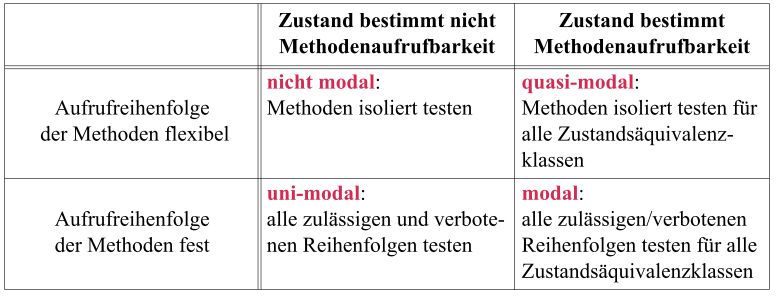
\includegraphics[width=0.85\textwidth]{4_6}
\end{figure}

\paragraph{Vorüberlegungen zur Realisierung von Invarianten,...:}
\begin{itemize}
	\item die teuere Überprüfung von Invarianten, ... muss durch ''Compile''-Flag abschaltbar sein (entweder systemweit oder je Subsystem)
	\item die Überprüfungen dürfen das Verhalten des ausführbaren Programms (abgesehen von Laufzeit und Speicherplatzverbrauch) nicht veränder 
	\item bei abgeschalteten Überprüfungen sollte soweit möglich der Code für diese Überprüfungen nicht Bestandteil des ausführbaren Programms sein
	\item die Reaktion auf fehlgeschlagene Überprüfungen muss an einer Stelle (veränderbar) festgelegt werden (Programmabbruch, Ausnahmeerweckung, ... )
	\item die Überprüfungen sollten möglichst lesbar niedergeschrieben werden
	\item Invarianten werden auch vor der Ausführung einer Methode und nach der Ausführung von ''Observer''-Methoden überprüft (um illegale Objektzugriffe entdecken zu können)
\end{itemize}

\paragraph{Zusicherungen (Assertions) in Java:}
\begin{itemize}
	\item Java besitzt ab Version 1.4 „assert“-Statement, das für den Einbau von Überprüfungen (Vor-/Nachbedingungen, Invarianten) genutzt wird
	\item die Überprüfung von ''assert''-Statements kann durch Runtime-Flags generell oder klassenweise an- bzw. abgeschaltet werden (''-enableassertions'' = ''-ea'' und ''.-disableassertions'' = ''-da'')
	\item die Überprüfungen sollten das Verhalten des ausführbaren Programms (abgesehen von Laufzeit und Speicherplatzverbrauch) nicht verändern (der Programmierer muss das sicherstellen)
	\item soll der Code für ''assert''-Statements nicht Bestandteil des ausführbaren Programms sein, so muss der Compiler davon ''überzeugt'' werden, dass der Code wegoptimiert werden kann
	\item ''assert''-Verletzungen können als ''AssertionError''-Ausnahmen abgefangen werden (und damit im Code festgelegte Reaktionen auslösen)
\end{itemize}

\paragraph{Einsatz von Automaten (Statecharts) zur Testplanung:}

Oft lassen sich die Vorbedingungen für den Aufruf von Methoden besser durch ein Statechart (hierarchischer Automat, siehe Software Eng. - Einführung) darstellen. Ein solches Statechart kann dann - ähnlich wie ein Kontrollflussgraph - zur Planung von Testfällen zur Berechnung von Testüberdeckungsmetriken herangezogen werden.

\begin{figure}[h]
	\centering
	\caption{Einsatz von Automaten (Statecharts) zur Testplanung}
	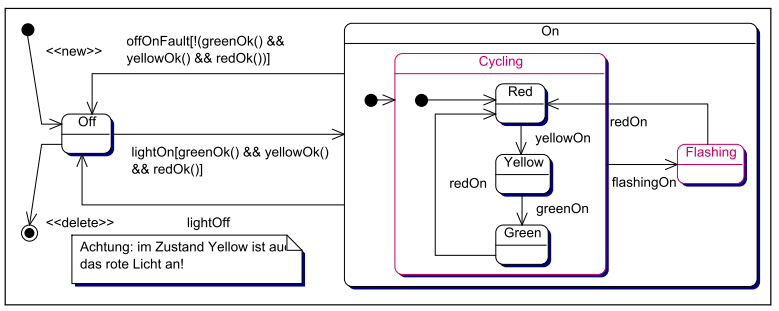
\includegraphics[width=0.85\textwidth]{4_6_1}
\end{figure}

\paragraph{Präzisierung der vier verschiedenen Arten von Klassen:}
\begin{itemize}
	\item Nicht modale Klasse:
	\begin{itemize}
		\item keine Methode der Klasse hat eine Vorbedingung über Attributen
		\item der Zustandsautomat der Klasse besteht aus einem Zustand
	\end{itemize}
	\item Quasimodale Klasse:
	\begin{itemize}
		\item mindestens eine Methode hat eine Vorbedingung über Attributen
		\item der Zustandsautomat der Klasse besteht aus einem Zustand
	\end{itemize}
	\item Unimodale Klasse:
	\begin{itemize}
		\item keine Methode der Klasse hat eine Vorbedingung über Attributen
		\item der Zustandsautomat der Klasse besteht aus mehreren Zuständen
	\end{itemize}
	\item Modale Klasse:
	\begin{itemize}
		\item mindestens eine Methode hat eine Vorbedingung über Attributen
		\item der Zustandsautomat der Klasse besteht aus mehreren Zuständen
	\end{itemize}
\end{itemize}

\paragraph{Definition von Testüberdeckungsmetriken für Statecharts:}
\begin{itemize}
	\item Tests müssen garantieren, dass alle Zustände mindestens einmal erreicht werden
	\item Tests müssen garantieren, dass jede Transition mindestens einmal ausgeführt wird
	\item Tests müssen garantieren, dass jede Transition mit allen sich wesentlich unterscheidenden Belegungen ihrer Bedingung ausgeführt wird
	\item Tests müssen alle möglichen Pfade durch Statechart (bis zu einer vorgegebenen Länge oder vorgegebenen Anzahl von Zyklen) ausführen
	\item zusätzlich zum Test aller explizit aufgeführten Transitionen werden für jeden Zustand alle sonst möglichen Ereignisse (Methodenaufrufe) ausgeführt 
\end{itemize}

\paragraph{Testplanung mit Transitionsbaum (Übergangsbaum) aus [Bi00]:}
\begin{enumerate}
	\item das gegebene Statechart wird in einen flachen Automaten übersetzt
	\item Transitionen mit komplexen Boole’schen Bedingungen werden in mehrere Transitionen mit Konjunktion atomarer Bedingungen übersetzt (Transition mit [(a1 \&\& a2) || (b1 \&\& b2)] wird ersetzt durch Transition mit [a1 \&\& a2] und Transition mit [b1 \&\& b2]
	\item ein Baum wird erzeugt, der
	\begin{itemize}
		\item initialen Zustand als Wurzelknoten (ersten, obersten Knoten) besitzt
		\item Zustandsknoten im Baum werden expandiert, indem alle Transitionen zu anderen Zuständen (und sich selbst) als Kindknoten hinzugefügt werden
		\item jeder Zustand wird nur einmal als Knoten im Transitionsbaum expandiert
	\end{itemize}
	\item jeder Pfad in dem Baum (von Wurzel zu einem Blatt) entspricht einer Testsequenz
	\item zusätzlich werden in jedem Zustand alle Ereignisse ausgelöst, die nicht im Transitionsbaum aufgeführt sind (spezifikationsverletzende Transitionen)
\end{enumerate}

\paragraph{Behandlung ereignisloser Transitionen:}

Automatenmodelle für die Verhaltensbeschreibung wie UML-Statecharts erlauben oft auch die Definition ereignisloser Transitionen. Diese werden wie folgt beim Testen behandelt:


\begin{itemize}
	\item Transition \textbf{ohne Ereignis mit Bedingung} [b]: sobald die Bedingung erfüllt ist, schaltet die Transition; beim Aufstellen von Testsequenzen sind zwei Fälle zu unterscheiden (zwei Unterbäume im Transitionsbaum):
	\begin{itemize}
		\item Bedingung b ist bereits erfüllt, wenn Startzustand der Transition betreten wird (Transition wird mit der Bedingung ''[b == true]'' markiert und schaltet sofort bei der Testausführung)
		\item Bedingung ist nicht erfüllt, wenn Startzustand betreten wird; wird später aber erfüllt (Transition wird mit Ereignis ''b -> true'' markiert und schaltet sobald die Bedingung b erfüllt ist)
	\end{itemize}
	\item Transition \textbf{ohne Ereignis und ohne Bedingung}: die Transition schaltet, sobald der Startzustand betreten wird: der Startzustand erhält im Transitionsbaum eine ausgehende Kante/Transition ohne Markierung
\end{itemize}

\paragraph{Ausführung der Testsequenzen:}
\begin{itemize}
	\item \textbf{Testvorbereitung}: Objekt muss in initialen Zustand (zurück-)versetzt werden
	\item \textbf{Testausführung} einer Sequenz von Methodenaufrufen (Testvektor): es wird unterschieden 
	\begin{itemize}
		\item \textbf{white-box-Sicht}: es gibt Zugriffsoperationen für Abfrage des internen Zustands; man kann also am Ende einer Testsequenz abfragen, ob richtiger Zustand erreicht wurde (interne Zustände der Implementierung müssen mit ''extern'' definierten Zuständen korrespondieren)
		\item \textbf{black-box-Sicht}: Aussenverhalten muss überprüft werden
	\end{itemize}
	\item \textbf{Testbeendigung}: ggf. wird Sequenz von Methodenaufrufen so vervollständigt, dass am Ende der Ausführung Objekt sich in einem ''terminalen'' Zustand befindet
	\item \textbf{Kombination} von Testsequenzen: um Aufwand für Initialisierung zu reduzieren, werden möglichst lange Testsequenzen generiert bzw. kombiniert
\end{itemize}

\paragraph{Abschließende Checkliste für Klassentest nach [Bi00]:}
\begin{itemize}
	\item jede Methode (auch die geerbten) wird mindestens einmal ausgeführt
	\item  alle Methodenparameter und alle nach aussen sichtbaren Attribute werden mit geeigneter Äquivalenzklassenbildung durchgetestet
	\item alle auslösbaren (ausgehenden) Ausnahmen werden mindestens einmal ausgelöst
	\item alle von gerufenen Methoden auslösbaren (eingehenden) Ausnahmen werden mindestens einmal behandelt (oder durchgereicht)
	\item alle identifizierten Objektzustände (auch hier Äquivalenzklassenbildung) werden beim Testen erreicht
	\item jede zustandsabhängige Methode wird in jedem Zustand ausgeführt (auch in den Zuständen, in denen ihr Aufruf nicht zulässig ist)
	\item alle möglichen Zustandsübergänge (mit allen Kombinationen von Bedingungen an den Übergängen) werden aktiviert
	\item zusätzlich werden die üblichen Performanz-, Last-, ... -Tests durchgeführt
\end{itemize}

\subsection{Mutationsbasierte Testverfahren}

\paragraph{Hypothesen}
\begin{itemize}
	\item Programmierer erstellen (oft) annährend korrekte Programme (Competent Programmer Hypothesis)
	\item Komplexe Fehler bedingen häufig die Existenz von simplen Fehlern (Coupling Effect)
\end{itemize}
\paragraph{Schlussfolgerungen}
\begin{itemize}
	\item Typische Programmierfehler lassen sich oft auf kleine syntaktische Änderungen (Mutationen) eines korrekten Programmes zurückführen
	\item Solche Programmmutationen lassen sich automatisiert durchführen
	\item Testfälle sind ''gut'', die bei gleichen Eingaben zu unterschiedlichen Ausgaben (unterschiedlichem Verhalten) eines Programms und eines seiner Mutanten führen
\end{itemize}

\paragraph{Anforderungen an (stark-)mutationserkennende Testfälle}

Der gesuchte Testfall soll bei seiner Ausführung
\begin{itemize}
	\item die fehlerhafte Stelle erreichen (\textbf{Reachability Condition}),
	\item der Programmzustand soll infiziert werden (\textbf{Infection Condition}), also während der Ausführung zu veränderten Variablenbelegungen führen
	\item und der infizierte Programmzustand soll in das Ergebnis propagiert werden (\textbf{Propagation Condition}), dieses also verändern.
\end{itemize}
\textbf{Achtung:}
\begin{itemize}
	\item Ist die ''Propagation Condition'' erfüllt, dann ist auch die ''Infection Condition'' zwangsläufig erfüllt.
	\item Ist die ''Infection Condition'' erfüllt, dann ist auch die ''Reachability Condition'' zwangsläufig erfüllt.
	\item Bislang für die Auswahl von Testfällen benutzte Programmüberdeckungs kriterien konzentrieren sich auf die ''Reachability Conditions''
\end{itemize}

\paragraph{Mutationsbasierte Testsuite-Bewertung:}
\begin{itemize}
	\item gegeben ist ein potentiell fehlerhaftes Programm p und eine \textbf{Test-Suite} TS, die aus einer Menge von Testfällen ${tc1, tc2, ... }$ besteht
	\item zunächst wird eine Menge von \textbf{Mutanten} $M = {m1, m2, ... }$ erzeugt, die sich in der Regel jeweils nur an einer Programmstelle vom Originalprogramm p unterscheiden (Programme mi mit mehreren Unterschieden gegenüber p werden \textbf{Mutanten höherer Ordnung} genannt)
	\item dann werden alle Testfälle der Test-Suite TS auf dem Programm $p$ und der Menge seiner Mutanten $M$ ausgeführt
	\item die Test-Suite bzw. ein Testfall tötet einen Mutanten $m_i$ , falls die Ausführung von $p$ und $m_i$ unterschiedliche Ausgaben erzeugen
	\item \textbf{Effektivität} einer Test-Suite: Anzahl der getöteten Mutanten
	\item \textbf{Effizienz} einer Test-Suite: Anzahl der benötigten Testfälle
	\item Erhöhung der Effizienz einer Test-Suite ohne Reduktion ihrer Effektivität: Testfälle, die keinen Mutanten töten, werden eliminiert; gleiches gilt für Teilmengen von Testfällen, die alle den selben Mutanten töten)
\end{itemize}

\paragraph{Mutationsbasierte Testsuite-Generierung:}

Die werkzeuggestützte Erzeugung von Testfällen, die bestimmte Mutanten töten, ist ein ''schwieriges'' Problem (i.A. nicht berechenbar).

\begin{itemize}
	\item naiver Ansatz: zufallsgesteuerte Erzeugung von Testfällen
	\item verifikationsbasierter Ansatz: das Problem der Erzeugung eines (fehlenden) Testfalles, der einen bestimmten Mutanten m eines Programms p tötet, wird in ein Verifikationsproblem übersetzt:
	\begin{itemize}
		\item erzeugt wird ein neues Programm, das p und m  hintereinander ausführt und die Ausgaben der Ausführung von p und m in verschiedenen Variablen speichert
		\item verifiziert wird dann die Eigenschaft des neuen Programms, für alle möglichen Eingaben bei der Ausführung von p und m immer die gleichen Ausgaben zu produzieren
		\item jedes von einem Verifikationswerkzeug produzierte Gegenbeispiel zu dieser Eigenschaft legt einen Testfall fest, der den Mutanten m tötet
	\end{itemize}
\end{itemize}

\paragraph{Bewertung des Ansatzes [ABL05]:}
\begin{itemize}
	\item Ähnlichkeit zwischen mechanisch erzeugten Mutanten und realen Fehlern ist größer als zwischen manuell eingebauten Fehlern und realen Fehlern
	\item bei manuell eingebauten Fehlern wird die Erkennungsrate einer Test-Suite unterschätzt (manuell eingebaute Fehler sind oft schwerer zu detektieren als mechanisch erzeugte Mutationen)
	\item (ausgewählte) Mutanten sind nicht einfacher oder schwerer zu detektieren als reale Fehler
\end{itemize}

\subsection{Testmanagement und Testwerkzeuge}
Testen wird nach [SL19] immer wie folgt durchgeführt:
\begin{itemize}
	\item \textbf{Testplanung}: es werden die zum Einsatz kommenden Methoden und Werkzeuge sowie die zu testenden Objekte  in einem Testkonzept festgelegt
	\item \textbf{Testüberwachung und Teststeuerung}: Durchführung, Protokollierung und Bewertung der folgenden Aktivitäten inklusive Entscheidung über Testende
	\item \textbf{Testanalyse}: es wird festgelegt was genau zu testen ist durch Überprüfung vorhandener Anforderungspezifikationen, Testobjekte, ...
	\item \textbf{Testentwurf}: es wird festgelegt wie getestet wird; dabei werden abstrakte (mit Bedingungen für Eingabewerte) oder konkrete Testfälle (mit konkreten Eingabewerten) spezifiziert
	\item \textbf{Testrealisierung}: es werden die spezifizierten Testfälle implementiert
	\item \textbf{Testdurchführung}: die ausgewählten Testfälle werden ausgeführt
	\item \textbf{Testabschluss}: es werden die Ergebnisse der vorangegangenen Aktivitäten zusammengetragen und konsolidiert
\end{itemize}

\paragraph{Aufgaben, Qualifikationen und Rollen nach [SL19]:}
\begin{itemize}
	\item \textbf{Testmanager} (Leiter): ist für Management der Testaktivitäten, der Testressourcen und die Bewertung des Testobjekts (gegenüber Projektmanager) verantwortlich
	\item \textbf{Testdesigner} (Analyst): erstellt Testspezifikationen und ermittelt Testdaten [ Ergänzung: könnte beim modellbasierten Testen auch für die Erstellung von Testmodellen und Festlegung von Überdeckungskriterien zuständig sein ]
	\item \textbf{Testfallgenerator}: werden Testfälle aus Modellen bzw. Spezifikationen automatisch erzeugt, so bedarf es einer weiteren Rolle, die die Testfallgenerierung mit Werkzeugunterstützung durchführt
	\item \textbf{Testautomatisierer}: realisiert die automatisierte Durchführung der spezifizierten Testfälle durch ausgewählte Testwerkzeuge
	\item \textbf{Testadministrator}: stellt die Testumgebung mit ausgewählten Testwerkzeugen zur Verfügung (zusammen Systemadministratoren etc.)
	\item \textbf{Tester}: ist für Testdurchführung, -protokollkierung und -auswertung zuständig (entspricht ''Certified Tester Foundation Level''-Kompetenzen) 
\end{itemize}


\paragraph{Weitere Aspekte des Testmanagements nach [SL19]:}
\begin{itemize}
	\item Betrachtung von \textbf{Kosten- und Wirtschaftlichkeitsaspekten}
	\begin{itemize}
		\item Ermittlung und AbschätzunTeststrategieg von Fehlerkosten
		\item Ermittlung und Abschätzung von Testkosten / Testaufwand
	\end{itemize}
	\item Wahl einer \textbf{}
	\begin{itemize}
		\item proaktiv vs. reaktiv (Testmanagement startet mit Projektbeginn vs. Testaktivitäten werden erst nach der Erstellung der Software gestartet)
		\item Testerstellungsansatz / Überdeckungskriterien / ...
		\item Orientierung an Standards für Vorgehensmodelle
	\end{itemize}
	\item Testen und \textbf{Risiko}
	\begin{itemize}
		\item Risiken beim Testen (Ausfall von Personal, ... )
		\item Risikobasiertes Testen (Fokus auf Minimierung von Produktrisiken)
	\end{itemize}
\end{itemize}

\paragraph{Meldung von Fehlern/Fehlermanagement:}
Es müssen alle Informationen erfasst werden, die für das Reproduzieren eines Fehlers notwendig sind. Eine Fehlermeldung kann wie folgt aufgebaut sein:
\begin{itemize}
	\item \textbf{Status}: Bearbeitungsfortschritt der Meldung (Neu, Offen, Analyse, Abgewiesen, Korrektur, Test, Erledigt)
	\item \textbf{Klasse}: Klassifzierung der Schwere des Problems (Menschenleben in Gefahr, Systemabsturz mit Datenverlust, ... , Schönheitsfehler)
	\item \textbf{Priorität}: Festlegung der Dringlichkeit, mit der Fehler behoben werden muss (sofort, da Arbeitsablauf blockiert beim Anwender, ... )
	\item \textbf{Anforderung}: die Stelle(n) in der Anforderungsspezifikation, auf die sich der Fehler bezieht
	\item \textbf{Fehlerquelle}: in welcher Softwareentwicklungsphase wurde der Fehler begangen
	\item \textbf{Fehlerart}: Berechnungsfehler, ...
	\item \textbf{Testfall}: genaue Beschreibung des Testfalls, der Fehler auslöst
	\item ...
\end{itemize}

\paragraph{Arten von Testwerkzeugen:}
Testwerkzeuge werden oft ''\textbf{Computer-Aided Software Test}''-Werkzeuge genannt (\textbf{CAST-Tools}). Man unterscheidet folgene Arten von CAST-Tools:
\begin{itemize}
	\item Werkzeuge zum \textbf{Testmanagement} und zur Testplanung: Erfassen von Testfällen, Abgleich von Testfällen mit Anforderungen, Verwaltung und (statistische) Auswertung von Fehlermeldungen, ...
	\item Werkzeuge zur \textbf{Testspezifikation}: Testdaten und Soll-Werte für zugehörige Ergebnisse werden (manuell) festgelegt und verwaltet
	\item \textbf{Testdatengeneratoren}: aus Softwaremodellen, Code, Grammatiken, ... werden automatisch Testdaten generiert
	\item \textbf{Testtreiber}: passend zu Schnittstellen von Testobjekten werden Testtreiber bzw. Testrahmen zur Verfügung gestellt, die die Aufruf von Tests mit Übergabe von Eingabewerten, Auswertung der Ergebnisse etc. abwickeln
	\item \textbf{Simulatoren}: bilden möglichst realitätsnah Produktionsumgebung nach (mit Simulation von anderen Systemen, Hardware, ... )
	\item \textbf{Testroboter} (Capture \& Replay-Werkzeug): zeichnet interaktive Benutzung einer Bedienungsoberfläche auf und kann Dialog wieder abspielen (solange sich Oberfläche nicht zu stark verändert)
	\item Werkzeuge für Last- und \textbf{Performanztests} (dynamische Analysen): Laufzeitmessungen, Speicherplatzverbrauch, ...
	\item \textbf{Komparatoren}: vergleichen erwartete mit tatsächlichen Ergebnissen, filtern unwesentliche Details, können ggf. auch Zustand von Benutzeroberflächen prüfen
	\item \textbf{Code-Überdeckungsanalysatoren}: für gewählte Überdeckungsmetriken wird Buch darüber geführt, wieviel Prozent Überdeckung erreicht ist, welche Programmausschnitte noch nicht überdeckt sind
	\item Werkzeuge für \textbf{statische Analysen}: Berechnung von Metriken, Kontroll- und Datenflussanomalien, ...
\end{itemize}

\subsection{Zusammenfassung}
Dynamische Programmanalysen und das ''traditionelle'' Testen sind die wichtigsten Mittel der analytischen Qualitätssicherung. Mindestens folgende Maßnahmen sollten immer durchgeführt werden:
\begin{itemize}
	\item Suche nach Speicherlecks und Zugriff auf nichtinitialisierte Speicherbereiche (oder falsche Speicherbereiche) mit geeigneten Werkzeugen
	\item automatische Regressions-Testdurchführung mit entsprechenden Frameworks zur Testautomatisierung
	\item Überprüfung der Zweigüberdeckung durch Testfälle anhand von Kontrollflussgraph (durch Werkzeuge)
	\item Verwendung von ''Black-Box''-Testverfahren mit Äquivalenzklassenbildung für Eingabeparameter (Objekte) zur Bestimmung von Testfällen
	\item Einbau möglichst vieler abschaltbarer Konsistenzprüfungen in Code (Vor- und Nachbedingungen) und ggf. defensive Programmierung
\end{itemize}





	\section{Management der Software-Entwicklung}

\paragraph{Themen dieses Kapitels}
\begin{itemize}
	\item bessere/modernere Prozessmodelle
	\item Verbesserung/Qualität von Softwareprozessmodellen
	\item Projektmanagement(-werkzeuge)
	\item optional: Kostenschätzung für Softwareprojekte
\end{itemize}

Viele im folgenden vorgestellten Überlegungen sind nicht ausschließlich für \textbf{Software} Entwicklungsprozesse geeignet, sondern werden ganz allgemein für die Steuerung komplexer technischer Entwicklungsprozesse eingesetzt.

\paragraph{Aufgaben des Managements:}
\begin{itemize}
	\item \textbf{Planungsaktivitäten}: Ziele definieren, Vorgehensweisen auswählen, Termine fest legen, Budgets vorbereiten, ...
	\begin{itemize}
		\item Vorgehensmodelle, Kostenschätzung, Projektpläne
	\end{itemize}
	\item \textbf{Organisationsaktivitäten}: Strukturieren von Aufgaben, Festlegung organisatorischer Strukturen, Definition von Qualifikationsprofilen für Positionen, ...
	\begin{itemize}
		\item Rollenmodelle, Team-Modelle, Projektpläne
	\end{itemize}
	\item \textbf{Personalaktivitäten}: Positionen besetzen, Mitarbeiter beurteilen, weiterbilden, ...
	\begin{itemize}
		\item nicht Thema dieser Vorlesung
	\end{itemize}
	\item  \textbf{Leitungsaktivitäten}: Mitarbeiter führen, motivieren, koordinieren, ...
	\begin{itemize}
		\item nicht Thema dieser Vorlesung
	\end{itemize}
	\item  \textbf{Kontrollaktivitäten}: Prozess- und Produktstandards entwickeln, Berichts- und Kontrollwesen etablieren, Prozesse und Produkte vermessen, Korrekturen, ...
	\begin{itemize}
		\item Qualititätsmanagement, insbesondere für Software-Entwicklungsprozesse
	\end{itemize}
\end{itemize}

\paragraph{Ziele des Managements}

Hauptziel des Projektmanagements ist die \textbf{Erhöhung der Produktivität}! 
\\ 
\\
\textbf{Allgemeine Definition von Produktivität:} Produktivität = Produktwert / Aufwand (oder: Leistung / Aufwand)
\\
\\
\textbf{Für Software-Entwicklung oft verwendete Definition:} Produktivität = Größe der Software / geleistete Mitarbeitertage
\begin{itemize}
	\item Maß für Größe der Software
	\item Berücksichtigung der Produktqualität
	\item Aufwand = Mitarbeitertage ?
	\item Nutzen (Return Of Investment) = Größe der Software ?
\end{itemize}

\paragraph{Einflussfaktoren für Produktivität [ACF97]:}
Angabe der Form ''+ 1 : X'' steht für Produktivitätssteigerung um maximal Faktor X \\
Angabe der Form ''- 1 : Y'' steht für Produktivitätsminderung um maximal Faktor Y.
\begin{itemize}
	\item Werkzeug-Einsatz: + 1 : 1,6
	\item Geeignete Methoden: + 1 : 1,9
	\item Produktkomplexität: - 1 : 2,4
	\item Hohe Zuverlässigkeitsanforderung: - 1 : 1,9
	\item Firmenkultur (corporate identity): + 1 : 11
	\item Arbeitsumgebung (eigenes Büro, abschaltbares Telefon, ... ): + 1 : ???
	\item Begabung der Mitarbeiter: + 1 : 10
	\item Erfahrung im Anwendungsgebiet: + 1 : 1,6
	\item Bezahlung, Berufserfahrung: kein messbarer Einfluss
\end{itemize}

\subsection{''Neuere'' Vorgehensmodelle}
Die naheliegendste Idee zur Verbesserung des Wasserfallmodells ergibt sich durch die Einführung von \textbf{Zyklen} bzw. \textbf{Rückgriffen}. Sie erlauben Wiederaufnehmen früherer Phasen, wenn in späteren Phasen Probleme auftreten.
\paragraph{Weitere Vorgehensmodelle:}
\begin{itemize}
	\item das V-Modell (umgeklapptes Wasserfallmodell)
	\item das evolutionäre Modell (iteriertes Wasserfallmodell)
	\item Rapid Prototyping (Throw-Away-Prototyping)
\end{itemize}

\paragraph{Probleme mit dem Wasserfallmodell insgesamt:}
\begin{itemize}
	\item Wartung mit ca. 60\% des Gesamtaufwandes ist eine Phase
	\begin{itemize}
		\item andere Prozessmodelle mit Wartung als eigener Entwicklungsprozess
	\end{itemize}
	\item zu Projektbeginn sind nur ungenaue Kosten- und Ressourcenschätzungen möglich
	\begin{itemize}
		\item Methoden zur Kostenschätzung anhand von Lastenheft (Pflichtenheft)
	\end{itemize}
	\item ein Pflichtenheft kann nie den Umgang mit dem fertigen System ersetzen, das erst sehr spät entsteht (Risikomaximierung)
	\begin{itemize}
		\item andere Prozessmodelle mit Erstellung von Prototypen, ...
	\end{itemize}
	\item Anforderungen werden früh eingefroren, notwendiger Wandel (aufgrund organisatorischer, politischer, technischer, ... Änderungen) nicht eingeplant
	\begin{itemize}
		\item andere Prozessmodelle mit evolutionärer Software-Entwicklung
	\end{itemize}
	\item strikte Phaseneinteilung ist unrealistisch (Rückgriffe sind notwendig)
	\begin{itemize}
		\item andere Prozessmodelle mit iterativer Vorgehensweise
	\end{itemize}
\end{itemize}

\begin{figure}[h]
	\centering
	\caption{Evolutionäres Modell (evolutionäres Prototyping)}
	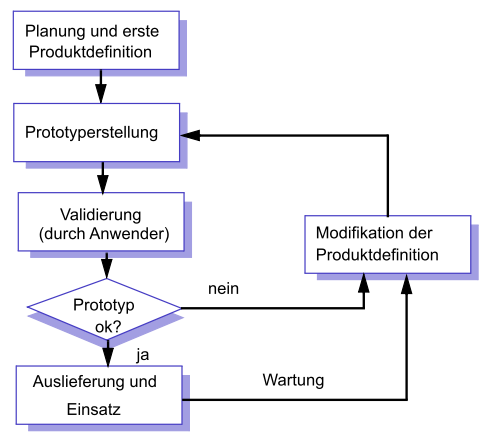
\includegraphics[width=0.5\textwidth]{5_1_1}
\end{figure}

\paragraph{Bewertung des evolutionären Modells:}
\begin{itemize}
	\item \textbf{Vorteile:}
	\begin{itemize}
		\item es ist sehr früh ein (durch Kunden) evaluierbarer Prototyp da
		\item Kosten und Leistungsumfang des gesamten Softwaresystems müssen nicht zu Beginn des Projekts vollständig festgelegt werden
		\item Projektplanung vereinfacht sich durch überschaubarere Teilprojekte
		\item  Systemarchitektur muss auf Erweiterbarkeit angelegt sein
	\end{itemize}
	\item \textbf{Nachteile:}
	\begin{itemize}
		\item es ist schwer, Systemarchitektur des ersten Prototypen so zu gestalten, dass sie alle später notwendigen Erweiterungen erlaubt
		\item Prozess der Prototyperstellung nicht festgelegt: Spiralmodell von Berry Böhm integriert Phasen des Wasserfallmodells
		\item evolutionäre Entwicklung der Anforderungsdefinition birgt Gefahr in sich, dass bereits realisierte Funktionen hinfällig werden
		\item  Endresultat sieht ggf. wie Software nach 10 Jahren Wartung aus
	\end{itemize}
\end{itemize}

\paragraph{Rapid Prototyping (Throw-Away-Prototyping):}
Mit Generatoren, ausführbaren Spezifikationssprachen, Skriptsprachen etc. wird:
\begin{itemize}
	\item Prototyp des Systems (seiner Benutzeroberfläche) realisiert
	\item dem Kunden demonstriert
	\item und anschließend weggeschmissen
\end{itemize}
\textbf{Bewertung:}
\begin{itemize}
	\item erlaubt schnelle Klärung der Funktionalität und Risikominimierung
	\item Vermeidung von Missverständnissen zwischen Entwickler und Auftraggeber
	\item früher Test der Benutzerschnittstelle
\end{itemize}

\subsection{Rational Unified Process für UML}
\begin{figure}[h]
	\centering
	\caption{Firma IBM (ehemals Rational) dominiert(e) Entwicklung der Standard-OO-Modellierungssprache UML und des zugehörigen Vorgehensmodells.}
	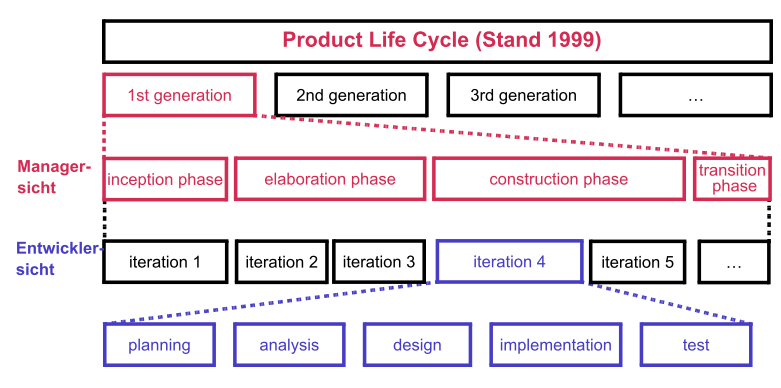
\includegraphics[width=0.85\textwidth]{5_2}
\end{figure}

\paragraph{Phasen der Lebenszyklusgeneration}
\begin{itemize}
	\item \textbf{Inception (Vorbereitung)}: Definition des Problembereichs und Projektziels für Produktgeneration mit Anwendungsbereichsanalyse (Domain Analysis) und Machbarkeitsstudie (für erste Generation aufwändiger)
	\begin{itemize}
		\item bei Erfolg weiter zu ...
	\end{itemize}
	\item \textbf{Elaboration (Entwurf)}: erste Anforderungsdefinition für Produktgeneration mit grober Softwarearchitektur und Projektplan (ggf. mit Rapid Prototyping)
	\begin{itemize}
		\item bei Erfolg weiter zu ...
	\end{itemize}
	\item  \textbf{Construction (Konstruktion)}: Entwicklung der neuen Produktgeneration als eine Abfolge von Iterationen mit Detailanalyse, -design, ... (wie beim evolutionären Vorgehensmodell)
	\begin{itemize}
		\item bei Erfolg weiter zu ...
	\end{itemize}
	\item  \textbf{Transition (Einführung)}: Auslieferung des Systems an den Anwender (inklusive Marketing, Support, Dokumentation, Schulung, ... )
\end{itemize}

\paragraph{Eigenschaften des Rational Unified Prozesses (RUP):}
\begin{itemize}
	\item  \textbf{modellbasiert}: für die einzelnen Schritte des Prozesses ist festgelegt, welche Modelle (Dokumente) des Produkts zu erzeugen sind
	\item \textbf{prozessorientiert}: die Arbeit ist in eine genau definierte Abfolge von Aktivitäten unterteilt, die von anderen Teams in anderen Projekten wiederholt werden können.
	\item \textbf{iterativ und inkrementell}: die Arbeit ist in eine Vielzahl von Iterationen unterteilt, das Produkt wird inkrementell entwickelt.
	\item \textbf{risikobewusst}: Aktivitäten mit hohem Risiko werden identifiziert und in frühen Iterationen in Angriff genommen.
	\item \textbf{zyklisch}: die Produktentwicklung erfolgt in Zyklen (Generationen). Jeder Zyklus liefert eine neue als kommerzielles Produkt ausgelieferte Systemgeneration.
	\item \textbf{ergebnisorientiert}: jede Phase (Iteration) ist mit der Ablieferung eines definierten Ergebnisses meist zu einem konkreten Zeitpunkt (Meilenstein) verbunden
\end{itemize}

\paragraph{Faustregeln für die Ausgestaltung eines Entwicklungsprozesses:}
\begin{itemize}
	\item die Entwicklung einer \textbf{Produktgeneration} dauert höchstens 18 Monate
	\item eine \textbf{Vorbereitungsphase} dauert 3-6 Wochen und besteht aus einer Iteration
	\item eine \textbf{Entwurfsphase} dauert 1-3 Monate und besteht aus bis zu 2 Iterationen
	\item  eine \textbf{Konstruktionsphase} dauert 1-9 Monate und besteht aus bis zu 7 Iterationen
	\item eine \textbf{Einführungsphase} dauert 4-8 Wochen und besteht aus einer Iteration
	\item jede \textbf{Iteration} dauert 4-8 Wochen (ggf. exklusive Vorbereitungs- und Nachbereitungszeiten, die mit anderen Iterationen überlappen dürfen)
	\item das gewünschte \textbf{Ergebnis} (Software-Release) einer Iteration ist spätestens bei ihrem Beginn festgelegt (oft Abhängigkeit von Ergebnissen vorheriger Iterationen)
	\item die \textbf{geplante Zeit} für eine Iteration wird nie (höchstens um 50\%) überschritten
	\item innerhalb der Konstruktionsphase wird mindestens im wöchentlichen Abstand ein \textbf{internes Software-Release} erstellt
	\item  mindestens 40\% \textbf{Reserve} an Projektlaufzeit für unbekannte Anforderungen, ...
\end{itemize}

\paragraph{Anmerkungen zu den Arbeitsbereichen (Workflows) des RUP:}
\begin{itemize}
	\item \textbf{Business Modeling} befasst sich damit, das Umfeld des zu erstellenden Softwaresystems zu erfassen (Geschäftsvorfälle, Abläufe, ... )
	\item \textbf{Requirements (Capture)} befasst sich damit die Anforderungen an ein Softwaresystem noch sehr informell zu erfassen
	\item \textbf{Analysis/Design} präzisiert mit grafischen Sprachen (Klassendiagramme etc.) die Anforderungen und liefert Systemarchitektur
	\item \textbf{Implementation/Test} entspricht den Aktivitäten in den Phasen ''Codierung bis Integrationstest'' des Wasserfallmodells
	\item \textbf{Deployment} entspricht ''Auslieferung und Installation'' des Wasserfallmodells
	\item \textbf{Configuration Management} befasst sich mit der Verwaltung von Softwareversionen und -varianten
	\item \textbf{Project Management} mit der Steuerung des Entwicklungsprozesses selbst
	\item \textbf{Environment} bezeichnet die Aktivitäten zur Bereitstellung benötigter Ressourcen (Rechner, Werkzeuge, ... )
\end{itemize}

\paragraph{Bewertung des (Rational) Unified Prozesses:}
\begin{itemize}
	\item Vorteile
	\begin{itemize}
		\item Manager hat die grobe ''Inception-Elaboration-Construction-Transition''-Sicht
		\item Entwickler hat zusätzlich die feinere arbeitsbereichsorientierte Sicht
		\item Wartung ist eine Abfolge zu entwickelnder Produktgenerationen
		\item es wird endgültig die Illusion aufgegeben, dass Analyse, Design, ... zeitlich begrenzte strikt aufeinander folgende Phasen sind
		\item es gibt ''Open Unified Process'' im Eclipse Umfeld
	\end{itemize}
	\item Nachteile
	\begin{itemize}
		\item sehr komplexes Vorgehensmodell für modellbasierte SW-Entwicklung
		\item nicht mit Behördenstandards (V-Modell, ... ) richtig integriert
		\item Qualitätssicherung ist kein eigener Aktivitätsbereich
	\end{itemize}
\end{itemize}

\subsection{Leichtgewichtige Prozessmodelle}

Herkömmlichen Standards für Vorgehensmodelle zur Softwareentwicklung (V-Modell, RUP) wird vorgeworfen, dass
\begin{itemize}
	\item sie sehr starr sind
	\item Unmengen an Papier produzieren
	\item und nutzlos Arbeitskräfte binden
\end{itemize}
Deshalb werden seit einiger Zeit sogenannte ''leichtgewichtige'' Prozessmodelle (\textbf{light-weight processes}) unter dem Schlagwort ''Agile Prozessmodelle'' propagiert, die sinnlosen bürokratischen Overhead vermeiden wollen.
\begin{itemize}
	\item siehe separater Foliensatz zu dieser Thematik
\end{itemize}

\paragraph{Verbesserung der Prozessqualität}
Ausgangspunkt der hier vorgestellten Ansätze sind folgende Überlegungen:
\begin{itemize}
	\item Softwareentwicklungsprozesse sind selbst Produkte, deren Qualität überwacht und verbessert werden muss
	\item bei der Softwareentwicklung sind bestimmte Standards einzuhalten (Entwicklungsprozess muss dokumentiert und nachvollziehbar sein)
	\item es bedarf kontinuierlicher Anstregungen, um die Schwächen von Entwicklungsprozessen zu identifizieren und zu eliminieren
\end{itemize}


\textbf{Hier vorgestellte Ansätze:}
\begin{itemize}
	\item \textbf{ISO 9000 Normenwerk} (Int. Standard für die Softwareindustrie)
	\item \textbf{Capability Maturity Model} (CMM/CMMI) des Software Engineering 
	Institutes (SEI) an der Carnegie Mellon University
	\item ISO-Norm \textbf{SPiCE} integriert und vereinheitlicht CMM und ISO 9000
\end{itemize}

\paragraph{Qualitätssicherung mimt der ISO 9000:}
Das \textbf{ISO 9000 Normenwerk} legt für das Auftraggeber-Lieferantenverhältnis einen allgemeinen organisatorischen Rahmen zur Qualitätssicherung fest.
\\
\\
Das ISO 9000 Zertifikat bestätigt, dass die Verfahren eines Unternehmens der ISO 9000 Norm entsprechen.

\paragraph{Wichtige Teile:}
\begin{itemize}
	\item \textbf{ISO 9000-1}: allgemeine Einführung und Überblick
	\item \textbf{ISO 9000-3}: Anwendung von ISO 9001 auf Softwareproduktion
	\item \textbf{ISO 9001}: Modelle der Qualitätssicherung in Design/Entwicklung, Produktion, Montage und Kundendienst
	\item \textbf{ISO 9004}: Aufbau und Verbesserung eines Qualitätsmanagementsystems
\end{itemize}

\paragraph{Von ISO 9000-3 vorgeschriebene Dokumente:}
\begin{itemize}
	\item \textbf{Vertrag Auftraggeber - Lieferant:}  Tätigkeiten des Auftraggebers, Behandlung von Anforderungsänderungen, Annahmekriterien (Abnahmetest), ...
	\item \textbf{Spezifikation:} funktionale Anforderungen, Ausfallsicherheit, Schnittstellen, ... des Softwareprodukts
	\item \textbf{Entwicklungsplan:} Zielfestlegung, Projektmittel, Entwicklungsphasen, Management, eingesetzte Methoden und Werkzeuge, ...
	\item \textbf{Qualitätssicherungsplan:}  Qualitätsziele (messbare Größen), Kriterien für Ergebnisse v. Entwicklungsphasen, Planung von Tests, Verifikation, Inspektionen
	\item \textbf{Testplan:} Teststrategie (für Integrationstest), Testfälle, Testwerkzeuge, Kriterien für Testvollständigkeit/Testende
	\item \textbf{Wartungsplan:} Umfang, Art der Unterstützung, ...
	\item \textbf{Konfigurationsmanagement:} Plan für Verwaltung von Softwareversionen und Softwarevarianten
\end{itemize}

\paragraph{Von ISO 9000-3 vorgeschriebene Tätigkeiten:}
\begin{itemize}
	\item \textbf{Konfigurationsmanagement} für Identifikation und Rückverfolgung von Änderungen, Verwaltung parallel existierender Varianten
	\item \textbf{Dokumentenmanagement} für geordnete Ablage und Verwaltung aller bei der Softwareentwicklung erzeugten Dokumente
	\item \textbf{Qualitätsaufzeichungen} (Fehleranzahl oder Metriken) für Verbesserungen am Produkt und Prozess
	\item \textbf{Festlegung} von Regeln, Praktiken und Übereinkommen für ein Qualitätssicherungssystem
	\item \textbf{Schulung} aller Mitarbeiter sowie Verfahren zur Ermittlung des Schulungsbedarfes
\end{itemize}
\textbf{Zertifizierung:} Die Einhaltung der Richtlinien der Norm wird von unabhängigen Zertifizierungsstellen im jährlichen Rhythmus überprüft.

\paragraph{Bewertung von ISO 9000:}
\begin{itemize}
	\item Vorteile
	\begin{itemize}
		\item lenkt die Aufmerksamkeit des Managements auf Qualitätssicherung
		\item ist ein gutes Marketing-Instrument
		\item reduziert das Produkthaftungsrisiko (Nachvollziehbarkeit von Entscheidungen)
	\end{itemize}
	\item Nachteile
	\begin{itemize}
		\item Nachvollziehbarkeit und Dokumentation von Prozessen reicht aus
		\item keine Aussage über Qualität von Prozessen und Produkten
		\item (für kleine Firmen) nicht bezahlbarer bürokratischer Aufwand
		\item Qualifikation der Zertifizierungsstellen umstritten
		\item oft große Abweichungen zwischen zertifiziertem Prozess und realem Prozess
	\end{itemize}
\end{itemize}

\paragraph{Das Capability Maturity Model (CMM):}
Referenzmodell zur Beurteilung von Softwarelieferanten, vom Software Engineering Institute entwickelt
\begin{itemize}
	\item Softwareentwicklungsprozesse werden in \textbf{5 Reifegrade} unterteilt
	\item Reifegrad (\textbf{maturity}) entspricht Qualitätsstufe der Softwareentwicklung
	\item höhere Stufe beinhaltet Anforderungen der tieferen Stufen
\end{itemize}

\textbf{Stufe 1 - chaotischer initialer Prozess (ihr Stand vor dieser Vorlesung):}
\begin{itemize}
	\item Prozess-Charakteristika:
	\begin{itemize}
		\item unvorhersehbare Entwicklungskosten, -zeit und -qualität
		\item kein Projektmanagement, nur ''Künstler'' am Werke
	\end{itemize}
	\item notwendige Aktionen:
	\begin{itemize}
		\item Planung mit Kosten- und Zeitschätzung einführen
		\item Änderungs- und Qualitätssicherungsmanagement 
	\end{itemize}
\end{itemize}

\textbf{Stufe 2 - wiederholbarer intuitiver Prozess  (Stand nach dieser Vorlesung?):}
\begin{itemize}
	\item Prozess-Charakteristika:
	\begin{itemize}
		\item Kosten und Qualität schwanken, gute Terminkontrolle
		\item Know-How einzelner Personen entscheidend
	\end{itemize}
	\item notwendige Aktionen:
	\begin{itemize}
		\item Prozessstandards entwickeln
		\item Methoden (für Analyse, Entwurf, Testen, ... ) einführen
	\end{itemize}
\end{itemize}

\textbf{Stufe 3 - definierter qualitativer Prozess (Stand der US-Industrie 1989?):}
\begin{itemize}
	\item Prozess-Charakteristika:
	\begin{itemize}
		\item zuverlässige Kosten- und Terminkontrolle, schwankende Qualität
		\item institutionalisierter Prozess, unabhängig von Individuen
	\end{itemize}
	\item notwendige Aktionen:
	\begin{itemize}
		\item Prozesse vermessen und analysieren
		\item quantitative Qualitätssicherung
	\end{itemize}
\end{itemize}

\textbf{Stufe 4 - gesteuerter/geleiteter quantitativer Prozess:}
\begin{itemize}
	\item Prozess-Charakteristika:
	\begin{itemize}
		\item gute statistische Kontrolle über Produktqualität
		\item Prozesse durch Metriken gesteuert
	\end{itemize}
	\item notwendige Aktionen:
	\begin{itemize}
		\item instrumentierte Prozessumgebung (mit Überwachung)
		\item ökonomisch gerechtfertigte Investitionen in neue Technologien
	\end{itemize}
\end{itemize}

\textbf{Stufe 5 - optimierender rückgekoppelter Prozess:}
\begin{itemize}
	\item Prozess-Charakteristika:
	\begin{itemize}
		\item quantitative Basis für Kapitalinvestitionen in Prozessautomatisierung und -verbesserung
	\end{itemize}
	\item notwendige Aktionen:
	\begin{itemize}
		\item kontinuierlicher Schwerpunkt auf Prozessvermessung und -verbesserung (zur Fehlervermeidung)
	\end{itemize}
\end{itemize}

\paragraph{ISO 9000 und CMM im Vergleich}
\begin{itemize}
	\item Schwerpunkt der \textbf{ISO 9001} Zertifizierung liegt auf Nachweis eines Qualitätsmanagementsystems im Sinne der Norm
	\begin{itemize}
		\item allgemein für Produktionsabläufe geeignet
		\item genau ein Reifegrad wird zertifiziert
	\end{itemize}
	\item \textbf{CMM} konzentriert sich auf Qualitäts- und Produktivitätssteigerung des gesamten Softwareentwicklungsprozesses
	\begin{itemize}
		\item auf Softwareentwicklung zugeschnitten
		\item dynamisches Modell mit kontinuierlichem Verbesserungsdruck
	\end{itemize}
	\item ISO-Norm \textbf{SPiCE} integriert und vereinheitlicht CMM und ISO 9000 (als ISO/IEC 15504)
\end{itemize}

\paragraph{SPiCE = Software Process Improvement and Capability dEtermination:}
Internationale Norm für \textbf{Prozessbewertung} (und Verbesserung). Sie bildet einheitlichen Rahmen für Bewertung der Leistungsfähigkeit von Organisationen, deren Aufgabe Entwicklung oder Erwerb, Lieferung, Einführung und Betreuung von Software-Systemen ist. Norm legt Evaluierungsprozess und Darstellung der Evaluierungsergebnisse fest.

\paragraph{Unterschiede zu CMM:}
\begin{itemize}
	\item orthogonale Betrachtung von Reifegraden und Aktivitätsbereichen
	\item deshalb andere Definition der 5 Reifegrade (z.B. ''1'' = alle Aktivitäten eines Bereiches sind vorhanden, Qualität der Aktivitäten noch unerheblich, ... )
	\item jedem Aktivitätsbereich oder Unterbereich kann ein anderer Reifegrad zugeordnet werden
\end{itemize}

\paragraph{Aktivitätsbereich von SPiCE:}
\begin{itemize}
	\item \textbf{Customer-Supplier-Bereich:} 
	\begin{itemize}
		\item Aquisition eines Projektes (Angebotserstellung, ... )
		\item ...
	\end{itemize}
	\item \textbf{Engineering-Bereich:} 
	\begin{itemize}
		\item Software-Entwicklung (Anforderungsanalyse, ... , Systemintegration)
		\item Software-Wartung
	\end{itemize}
	\item \textbf{Support-Bereich:} 
	\begin{itemize}
		\item Qualitätssicherung
		\item ...
	\end{itemize}
	\item \textbf{Management-Bereich:} 
	\begin{itemize}
		\item Projekt-Management
		\item ...
	\end{itemize}
	\item \textbf{Organisations-Bereich:} 
	\begin{itemize}
		\item Prozess-Verbesserung
		\item ...
	\end{itemize}
\end{itemize}

\paragraph{CMMI = Capability Maturity Model Integration (neue Version von CMM):}
CMMI ist die \textbf{neue Version des Software Capability Maturity Model}. Es ersetzt nicht nur verschiedene Qualitäts-Modelle für unterschiedliche Entwicklungs-Disziplinen (z.B. für Software-Entwicklung oder System-Entwicklung), sondern integriert diese in einem neuen, modularen Modell. Dieses modulare Konzept ermöglicht zum einen die Integration weiterer Entwicklungs-Disziplinen (z.B. Hardware-Entwicklung), und zum anderen auch die Anwendung des Qualitätsmodells in übergreifenden Disziplinen (z.B. Entwicklung von Chips mit Software).
\\
\\
Geschichte von CMM und CMMI:
\begin{itemize}
	\item 1991 wird Capability Maturity Model 1.0 herausgegeben
	\item 1993 wird CMM überarbeitet und in der Version 1.1 bereitgestellt
	\item 1997 wird CMM 2.0 kurz vor Verabschiedung vom DoD zurückgezogen
	\item 2000 wird CMMI als Pilotversion 1.0 herausgegeben
	\item 2002 wird CMMI freigegeben
	\item Ende 2003 ist die Unterstützung von CMM ausgelaufen
\end{itemize}

\paragraph{Eigenschaften von CMMI:}
Es gibt \textbf{Fähigkeitsgrade} für einzelne Prozessgebiete (ähnlich zu SPiCE):
\begin{itemize}
	\item \textbf{0 - Incomplete:} 
	\begin{itemize}
		\item Ausgangszustand, keine Anforderungen
	\end{itemize}
	\item \textbf{1 - Performed: } 
	\begin{itemize}
		\item die spezifischen Ziele des Prozessgebiets werden erreicht
	\end{itemize}
	\item \textbf{2 - Managed:} 
	\begin{itemize}
		\item der Prozess wird gemanagt
	\end{itemize}
	\item \textbf{3 - Defined:} 
	\begin{itemize}
		\item der Prozess wird auf Basis eines angepassten Standard-Prozesses gemanagt und verbessert
	\end{itemize}
	\item \textbf{4 - Quantitatively Managed:} 
	\begin{itemize}
		\item der Prozess steht unter statistischer Prozesskontrolle
	\end{itemize}
	\item \textbf{5 - Optimizing:} 
	\begin{itemize}
		\item der Prozess wird mit Daten aus der statistischen Prozesskontrolle verbessert
	\end{itemize}
\end{itemize}

\paragraph{Eigenschaften von CMMI-Fortsetzung:}
Es gibt \textbf{Reifegrade}, die Fähigkeitsgrade auf bestimmten Prozessgebieten erfordern (ähnlich zu CMM):
\begin{itemize}
	\item \textbf{1- Initial:} 
	\begin{itemize}
		\item keine Anforderungen, diesen Reifegrad hat jede Organisation automatisch
	\end{itemize}
	\item \textbf{2 - Managed:} 
	\begin{itemize}
		\item die Projekte werden gemanagt durchgeführt und ein ähnliches Projekt kann erfolgreich wiederholt werden
	\end{itemize}
	\item \textbf{3 - Defined:} 
	\begin{itemize}
		\item die Projekte werden nach einem angepassten Standard-Prozess durchgeführt, und es gibt eine kontinuierliche Prozessverbesserung
	\end{itemize}
	\item \textbf{4 - Quantitatively Managed:} 
	\begin{itemize}
		\item es wird eine statistische Prozesskontrolle durchgeführt
	\end{itemize}
	\item \textbf{5 - Optimizing:} 
	\begin{itemize}
		\item die Prozesse werden mit Daten aus statistischen Prozesskontrolle verbessert
	\end{itemize}
\end{itemize}

\paragraph{Konsequenzen für die ``eigene'' Software-Entwicklung:}
Im Rahmen von Studienarbeiten, Diplomarbeiten, ... können Sie keinen CMM(I)-Level-5- oder SPiCE-Software-Entwicklungsprozess verwenden, aber:
\begin{itemize}
	\item Einsatz von Werkzeugen für \textbf{Anforderungsanalyse und Modellierung}
	\begin{itemize}
		\item in der Vorlesung ``Software-Engineering - Einführung'' behandelt
	\end{itemize}
	\item Einsatz von \textbf{Konfigurations- und Versionsmanagement-Software}
	\begin{itemize}
		\item wird in dieser Vorlesung behandelt
	\end{itemize}
	\item Einsatz von Werkzeugen für systematisches \textbf{Testen, Messen} der Produktqualität
	\begin{itemize}
		\item wird in dieser Vorlesung behandelt
	\end{itemize}
	\item Ergänzender Einsatz von ``\textbf{Extreme Programming}''-Techniken (z.B. ``Test first'')
	\item Einsatz von Techniken zur Verbesserung des ``persönlichen'' Vorgehensmodells
	\begin{itemize}
		\item siehe [Hu96] über den ``\textbf{Personal Software Process}''
	\end{itemize}
\end{itemize}

\subsection{Projektpläne und Projektorganisation}
Am Ende der Machbarkeitsstudie steht die Erstellung eines Projektplans mit
\begin{itemize}
	\item Identifikation der einzelnen \textbf{Arbeitspakete} 
	\item \textbf{Terminplanung} (zeitliche Aufeinanderfolge der Pakete)
	\item \textbf{Ressourcenplanung}  (Zuordnung von Personen zu Paketen, ... )
\end{itemize}
Hier wird am deutlichsten, dass eine Machbarkeitsstudie ohne ein grobes Design der zu erstellenden Software nicht durchführbar ist, da:
\begin{itemize}
	\item Arbeitspakete ergeben sich aus der Struktur der Software
	\item Abhängigkeiten und Umfang der Pakete ebenso
	\item Realisierungsart der Pakete bestimmt benötigte Ressourcen
\end{itemize}
\textbf{Konsequenz:} Projektplanung und -organisation ist ein fortlaufender Prozess. Zu Projektbeginn hat man nur einen groben Plan, der sukzessive verfeinert wird.

\paragraph{Terminologie:}
\begin{itemize}
	\item \textbf{Prozessarchitektur}  = grundsätzliche Vorgehensweise einer Firma für die Beschreibung von Software-Entwicklungsprozessen (Notation, Werkzeuge)
	\item \textbf{Prozessmodell} = Vorgehensmodell = von einer Firma gewählter Entwicklungsprozess (Wasserfallmodell oder RUP oder ... )
	\item \textbf{Projektplan} = an einem Prozessmodell sich orientierender Plan für die Durchführung eines konkreten Projektes
	\item \textbf{Vorgang} = Aufgabe = Arbeitspaket = abgeschlossene Aktivität in Projektplan, die
	\begin{itemize}
		\item bestimmte Eingaben (Vorbedingungen) benötigt und Ausgaben produziert
		\item Personal und (sonstige) Betriebsmittel für Ausführung braucht
		\item eine bestimmte Zeitdauer in Anspruch nimmt
		\item und Kosten verursacht und/oder Einnahmen bringt
	\end{itemize}
	\item \textbf{Phase} = Zusammenfassung mehrerer zusammengehöriger Vorgänge zu einem globalen Arbeitsschritt
	\item \textbf{Meilenstein} = Ende einer Gruppe von Vorgängen (Phase) mit besonderer Bedeutung (für die Projektüberwachung) und wohldefinierten Ergebnissen
\end{itemize}

\subsection{Aufwands- und Kostenschätzung}
Die \textbf{Kosten} eines Softwareproduktes und die \textbf{Entwicklungsdauer} werden im wesentlichen durch den personellen Aufwand bestimmt. Bislang haben wir vorausgesetzt, dass der personelle Aufwand bekannt ist, hier werden wir uns mit seiner Berechnung bzw. Schätzung befassen.
\\
\\
Der \textbf{personelle Aufwand} für die Erstellung eines Softwareproduktes ergibt sich aus
\begin{itemize}
	\item dem ''\textbf{Umfang}'' des zu erstellenden Softwareprodukts
	\item der geforderten \textbf{Qualität} für das Produkt
\end{itemize}
\textbf{Übliches Maß für Personalaufwand:} Mitarbeitermonate(MM) oder Mitarbeiterjahre (MJ): 1MJ = 10MM (wegen Urlaub, Krankheit,...)
\\
\textbf{Übliches Maß für Produktumfang:} ''LOC''

\paragraph{Schätzverfahren im Überblick:}
\begin{itemize}
	\item \textbf{Analogiemethode:} Experte vergleicht neues Projekt mit bereits abgeschlossenen ähnlichen Projekten und schätzt Kosten ''gefühlsmäßig'' ab
	\begin{itemize}
		\item Expertenwissen lässt sich schwer vermitteln und nachvollziehen
	\end{itemize}
	\item \textbf{Prozentsatzmethode:} aus abgeschlossenen Projekten wird Aufwandsverteilung auf Phasen ermittelt; anhand beendeter Phasen wird Projektrestlaufzeit geschätzt
	\begin{itemize}
		\item funktioniert allenfalls nach Abschluss der Analysephase
	\end{itemize}
	\item \textbf{Parkinsons Gesetz:}  die Arbeit ist beendet, wenn alle Vorräte aufgebraucht sind
	\begin{itemize}
		\item praxisnah, realistisch und wenig hilfreich ...
	\end{itemize}
	\item \textbf{Price to Win:} die Software-Kosten werden auf das Budget des Kundens geschätzt
	\begin{itemize}
		\item andere Formulierung von ``Parkinsons Gesetz'', führt in den Ruin ...
	\end{itemize}
	\item \textbf{Gewichtungsmethode:}  Bestimmung vieler Faktoren (Erfahrung der Mitarbeiter, verwendete Sprachen, ... ) und Verknüpfung durch mathematische Formel
	\begin{itemize}
		\item LOC-basierter Vertreter: COnstructive COst MOdel (COCOMO)
		\item FP-basierte Vertreter: Function-Point-Methoden in vielen Varianten
	\end{itemize}
\end{itemize}

\paragraph{Softwareumfang = Lines of Code?}
Die ''\textbf{Lines of Code}'' als Ausgangsbasis für die Projektplanung (und damit auch zur Überwachung der Produktivität von Mitarbeitern) zu verwenden ist fragwürdig, da:
\begin{itemize}
	\item Codeumfang erst mit Abschluss der Implementierungsphase bekannt ist
	\item selbst Architektur auf Teilsystemebene noch unbekannt ist
	\item Wiederverwendung mit geringeren LOC-Zahlen bestraft wird
	\item gründliche Analyse, Design, Testen, ... zu geringerer Produktivität führt
	\item Anzahl von Codezeilen abhängig vom persönlichen Programmierstil ist
	\item Handbücher schreiben, ... ungenügend berücksichtigt wird
\end{itemize}
\textbf{Achtung:} Die starke Abhängigkeit der LOC-Zahlen von einer Programmiersprache ist zulässig, da Programmiersprachenwahl (großen) Einfluss auf Produktivität hat.

\begin{table}
	\centering
	\begin{tabular}{||c | c | c | c | c | c||} 
		\hline
		  & Analyse & Design & Codierung & Test & Sonstiges \\  
		\hline\hline
		C & 3 Wochen & 5 Wochen & 8 Wochen & 10 Wochen & 2 Wochen \\ 
		\hline
		Smalltalk & 3 Wochen & 5 Wochen & 2 Wochen & 6 Wochen & 2 Wochen \\ 
		\hline
	\end{tabular}
	\caption{Einfluss von Programmiersprache auf Produktivität:}
\end{table}

\begin{table}
	\centering
	\begin{tabular}{||c | c | c | c ||} 
		\hline
		& Programmgröße & Aufwand & Produktivität \\  
		\hline\hline
		C & 3 2.000 LOC & 28 Wochen & 70 LOC/Woche \\ 
		\hline
		Smalltalk & 500 LOC & 18 Wochen & 27 LOC/Wochen \\ 
		\hline
	\end{tabular}
	\caption{Konsequenzen für die Gesamtproduktivität:}
\end{table}

\textbf{Fazit:}
\begin{itemize}
	\item Produktivität kann \textbf{nicht} in ''Lines Of Code pro Zeiteinheit'' sinnvoll gemessen werden (sonst wäre Programmieren in Assembler die beste Lösung)
	\item also: Vorsicht mit Einsatz von Maßzahlen (keine sozialistische Planwirtschaft)
\end{itemize}

\paragraph{Softwareumfang = Function Points!}
Bei der \textbf{Function-Point-Methode} zur Kostenschätzung wird der Softwareumfang anhand der Produktanforderungen aus dem Lastenheft geschätzt. Es gibt inzwischen einige Spielarten; hier wird (weitgehend) der Ansatz der \textbf{International Function Point Users Group (IFPUG)} vorgestellt.
\\
\\
Jede Anforderung wird gemäß IFPUG einer von 5 Kategorien zugeordnet [ACF97]:
\begin{enumerate}
	\item \textbf{Eingabedaten} (über Tastatur, CD, externe Schnittstellen, ... )
	\item \textbf{Ausgabedaten} (auf Bildschirm, Papier, externe Schnittstelle, ... )
	\item \textbf{Abfragen} (z.B. SQL-Queries auf einem internen Datenbestand)
	\item \textbf{Datenbestände} (sich ändernde interne Datenbankinhalte)
	\item \textbf{Referenzdateien} (im wesentlichen unveränderliche Daten)
\end{enumerate}
Dann werden \textbf{Function-Points (FPs)} berechnet, bewertet, ... .

\paragraph{Datenbestände = Internal Logical File (ILF) = Interne Entitäten:}
Unter einer \textbf{internen (Geschäfts-)Entität} definiert die IFPUG eine aus Anwendersicht logisch zusammengehörige Gruppe vom Softwaresystem verwalteter Daten, also z.B.:
\begin{itemize}
	\item eine Gruppe von Produktdaten des Lastenheftes in der Machbarkeitsstudie
	\item Klassen mit Attributen u. Beziehungen eines Paketes aus Modellen im Pflichtenheft in der Analysephase
\end{itemize}
Es werden Datenelementtypen (Attribute) sowie Entitätstypen (Klassen, Sätze) und zusätzlich Beziehungstypen (Assoziationen) gezählt. Anhand  dieser Zählung wird Komplexität eines Datenbestandes wie folgt bestimmt: \\
\textbf{einfach = 7 FPs, mittel = 10 FPs oder komplex = 15 FPs}

\begin{table}
	\centering
	\begin{tabular}{||c | c | c | c | c ||} 
		\hline
		\textbf{Interne Entitäten} & Anzahl Attribute <= 19 & 19 < Anzahl Attribute <= 50 & Anzahl Attribute > 50 \\  
		\hline\hline
		Klassen+Assoz. <= 1 & einfache Komplexität & einfache Komplexität & mittlere Komplexität \\ 
		\hline
		2 <= Klassen+Assoz. <= 5 & einfache Komplexität & mittlere Komplexität & hohe Komplexität \\ 
		\hline
		Klassen+Assoz. > 5 & mittlere Komplexität & hohe Komplexität & hohe Komplexität \\ 
		\hline
	\end{tabular}
	\caption{Interne Entitäten}
\end{table}

\paragraph{Referenzdateien = External Interface File = (EIF) = Externe Entitäten:}
Unter einer \textbf{externen (Geschäfts-)Entität} definiert die IFPUG eine aus Anwendersicht logisch zusammengehörige Gruppe vom System benutzter aber nicht selbst verwalteter Daten.
\\
\\
Wieder werden Datenelementtypen (Attribute) sowie Entitätstypen (Klassen, Sätze) und zusätzlich Beziehungstypen (Assoziationen) gezählt. Anhand  dieser Zählung wird Komplexität eines Datenbestandes wie folgt bestimmt: \\
\textbf{einfach = 5 FPs, mittel = 7 FPs oder komplex = 10 FPs}

\begin{table}
	\centering
	\begin{tabular}{||c | c | c | c | c ||} 
		\hline
		\textbf{Externe Entitäten} & Anzahl Attribute <= 19 & 19 < Anzahl Attribute <= 50 & Anzahl Attribute > 50 \\  
		\hline\hline
		Klassen+Assoz. <= 1 & einfache Komplexität & einfache Komplexität & mittlere Komplexität \\ 
		\hline
		2 <= Klassen+Assoz. <= 5 & einfache Komplexität & mittlere Komplexität & hohe Komplexität \\ 
		\hline
		Klassen+Assoz. > 5 & mittlere Komplexität & hohe Komplexität & hohe Komplexität \\ 
		\hline
	\end{tabular}
	\caption{Externe Entitäten}
\end{table}

Es werden weniger FPs als bei internen Entitäten vergeben, da die betrachteten Datenbestände nur eingelesen aber nicht verwaltet werden müssen.

\paragraph{(Externe) Eingabedaten = External Input (EI):}

\textbf{Eingabedaten} für \textbf{Elementarprozess}, der Daten oder Steuerinformationen des Anwenders verarbeitet, aber keine Ausgabedaten liefert. Es handelt sich dabei um den kleinsten selbständigen Arbeitsschritt in der Arbeitsfolge eines Anwenders, als etwa:
\begin{itemize}
	\item Produktfunktionen des Lastenheftes in der Machbarkeitsstudie
	\item ''Use Cases'' aus Pflichtenheft in der Analysephase
\end{itemize}
Gezählt werden für jeden Elementarprozess die Anzahl seiner als Eingabe verwendeten Entitätstypen (Klassen, Sätze) und deren Datenelementtypen (Attribute, Felder). Anhand dieser Zählung wird Komplexität des Elementarprozesses wie folgt bestimmt: \\
\textbf{einfach = 3 FPs, mittel = 4 FPs oder komplex = 6 FPs}

\begin{table}
	\centering
	\begin{tabular}{||c | c | c | c | c ||} 
		\hline
		\textbf{Externe Eingabe} & Anzahl Attribute <= 4 & 4 < Anzahl Attribute <= 15 & Anzahl Attribute > 15 \\  
		\hline\hline
		Anzahl Klassen <= 1 & einfache Komplexität & einfache Komplexität & mittlere Komplexität \\ 
		\hline
		Anzahl Klassen = 2 & einfache Komplexität & mittlere Komplexität & hohe Komplexität \\ 
		\hline
		Anzahl Klassen > 2 & mittlere Komplexität & hohe Komplexität & hohe Komplexität \\ 
		\hline
	\end{tabular}
	\caption{Externe Eingaben}
\end{table}

\paragraph{Externe Ausgaben = External Output (EO)}
Ausgabedaten eines \textbf{Elementarprozesses} (Produktfunktion, Use Case), der Anwender Daten oder Steuerinformationen liefert. Achtung: der Elementarprozess darf keine Eingabedaten benötigen; ansonsten handelt es sich um eine ''Externe Abfrage'' oder ... .
\\
\\
Gezählt werden für jeden Elementarprozess die Anzahl seiner als Ausgabe verwendeten Entitätstypen (Klassen, Sätze) und deren Datenelementtypen (Attribute, Felder). Anhand dieser Zählung wird Komplexität des Elementarprozesses wie folgt bestimmt:
\textbf{einfach = 4 FPs, mittel = 5 FPs oder komplex = 7 FPs}

\begin{table}
	\centering
	\begin{tabular}{||c | c | c | c | c ||} 
		\hline
		\textbf{Externe Ausgaben} & Anzahl Attribute <= 5 & 5 < Anzahl Attribute <= 19 & Anzahl Attribute > 19 \\  
		\hline\hline
		Anzahl Klassen <= 1 & einfache Komplexität & einfache Komplexität & mittlere Komplexität \\ 
		\hline
		2 <= Anzahl Klassen <= 3 & einfache Komplexität & mittlere Komplexität & hohe Komplexität \\ 
		\hline
		Anzahl Klassen > 3 & mittlere Komplexität & hohe Komplexität & hohe Komplexität \\ 
		\hline
	\end{tabular}
	\caption{Externe Ausgaben}
\end{table}

\paragraph{Externe Abfragen = External Inquiry (EQ):}
Betrachtet werden \textbf{Elementarprozesse} (Produktfunktion, Use Case), die anhand von Eingaben Daten des internen Datenbestandes ausgeben (ohne auf diesen Daten komplexe Berechnungen durchzuführen).
\\
\\
Nach den Regeln für ''Externe Eingaben'' werden die Eingabedaten bewertet, nach den Regeln für ''Externe Ausgaben'' die Ausgabedaten; anschließend wird die höhere Komplexität übernommen und wie folgt umgerechnet: \\
\textbf{einfach = 3 FPs, mittel = 4 FPs oder komplex = 6 FPs}
\\
\\
\textbf{Achtung:}  ein Elementarprozess, der Eingabedaten zur Suche nach intern gespeicherten Daten benötigt und vor der Ausgabe \textbf{komplexe Berechnungen} durchführt, wird anders behandelt. In diesem Fall wird nicht das Maximum gebildet, sondern die \textbf{Summe} der FPs von ''Externe Eingabe'' und ''Externe Ausgabe''.

\begin{figure}[h]
	\centering
	\caption{Überblick über die FP-Methode - 1 [Ba98]:}
	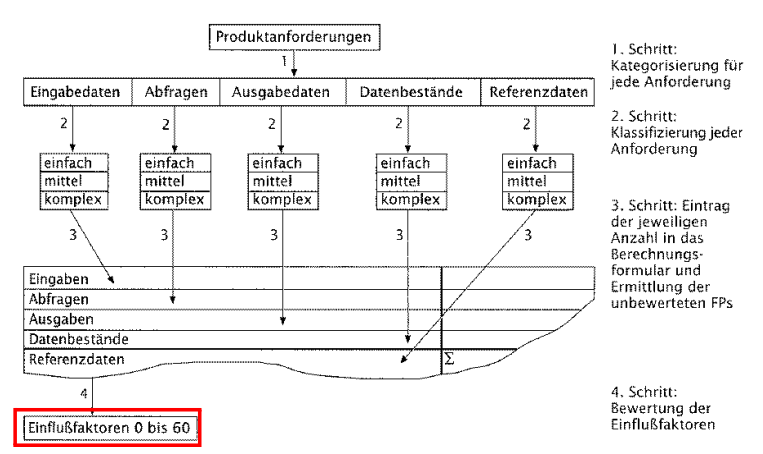
\includegraphics[width=0.85\textwidth]{5_5_1}
\end{figure}

\begin{figure}[h]
\centering
\caption{Überblick über die FP-Methode - 2:}
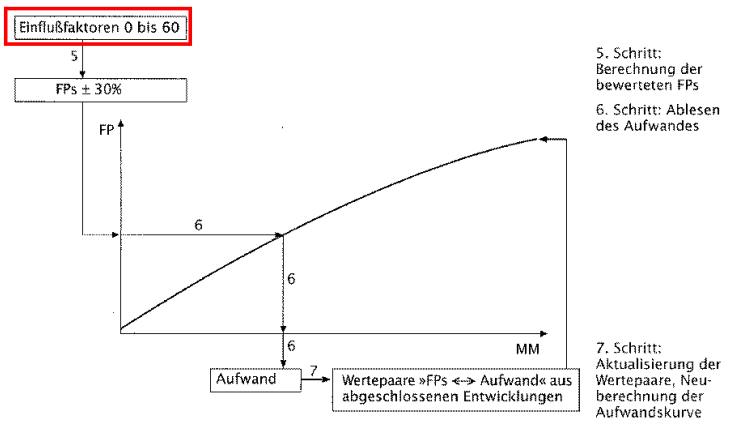
\includegraphics[width=0.85\textwidth]{5_5_2}
\end{figure}

\paragraph{Zusätzliche Einflussfaktoren:}
Die vorige Tabelle unterscheidet sieben Einflussfaktoren; andere Quellen nennen 14 bzw. \textbf{19 verschiedene Faktoren}, die Werte von 0 bis 5 erhalten (siehe [Hu99]):
\begin{enumerate}
	\item Komplexität der Datenkommunikation
	\item Grad der verteilten Datenverarbeitung
	\item geforderte Leistungsfähigkeit
	\item Komplexität der Konfiguration (Zielplattform)
	\item Anforderung an Transaktionsrate
	\item Prozentsatz interaktiver Dateneingaben
	\item geforderte Benutzerfreundlichkeit
	\item interaktive bzw. Online-Pflege des internen Datenbestandes
	\item Komplexität der Verarbeitungslogik
	\item geforderter Grad der Wiederverwendbarkeit
	\item benötigte Installationshilfen
	\item leichte Bedienbarkeit (Grad der Automatisierung der Bedienung)
	\item Mehrfachinstallationen (auf verschiedenen Zielplattformen)
	\item Grad der gefoderten Änderungsfreundlichkeit
	\item Randbedingungen anderer Anwendungen
	\item Sicherheit, Datenschutz, Prüfbarkeit
	\item Anwenderschulung
	\item Datenaustausch mit anderen Anwendungen
	\item Dokumentation
\end{enumerate}

\paragraph{Ermittlung der FP-Aufwandskurve:}
\begin{itemize}
	\item beim ersten Projekt muss man auf \textbf{bekannte Kurven} (für ähnliche Projekte) zurückgreifen (IBM-Kurve mit $FP = 26 * MM^{0,8}8$, VW AG Kurve, ... )
	\item alternativ kann man eigene abgeschlossene Projekte \textbf{nachkalkulieren}, allerdings:
	\begin{itemize}
		\item Nachkalkulationen sind aufwändig
		\item Dokumentation von Altprojekten oft unvollständig
		\item oft gibt es nur noch den Quellcode (keine Lasten- oder Pflichtenhefte)
		\item Kosten (Personenmonate) alter Projekte oft unklar (wurden Überstunden berücksichtigt, welche Aktivitäten wurden mitgezählt, ... )
	\end{itemize}
	\item das Verhältnis von MM zu FP bei abgeschlossenen eigenen Projekten wird zur nachträglichen ''\textbf{Kalibrierung}'' der Kurve benutzt:
	\begin{itemize}
		\item neues Wertepaar wird hinzugefügt oder neues Wertepaar ersetzt ältestes Wertepaar
		\item Frage: was für eine Funktion benutzt man für Interpolation von Zwischenwerten (meist nicht linear, sondern eher quadratisch oder gar exponentiell)
	\end{itemize}
\end{itemize}

\paragraph{Nachkalkulation von Projekten mit ''Backfiring''-Methode:}
Bei alten Projekten gibt es oft nur noch den Quellcode und keine Lasten- oder Pflichtenhefte, aus denen FPs errechnet werden können. In solchen Fällen versucht man FPs aus Quellcode rückzurechnen.
\\
\textbf{Achtung:} LOC in Programmiersprache X pro MM Codierung angeblich nahezu konstant -> damit ist z.B. Produktivität beim Codieren in Smalltalk 4 mal höher als in C

\paragraph{Vorgehensweise bei Kostenschätzung (mit FP-Methode):}
\begin{enumerate}
	\item Festlegung des verwendeten \textbf{Ansatzes}, Bereitstellung von Unterlagen
	\item \textbf{Systemgrenzen} festlegen (was gehört zum Softwaresystem dazu)
	\item \textbf{Umfang} des zu erstellenden Softwaresystems (in FPs) \textbf{messen}
	\item Umrechnung von Umfang (FPs) in \textbf{Aufwand} (MM) mit Aufwandskurve
	\item \textbf{Zuschläge} einplanen (für unvorhergesehene Dinge, Schätzungenauigkeit)
	\item Aufwand auf Phasen bzw. Iterationen \textbf{verteilen}
	\item Umsetzung in \textbf{Projektplan} mit Festlegung von \textbf{Teamgröße}
	\item Aufwandschätzung \textbf{prüfen} und dokumentieren
	\item Aufwandschätzung für Projekt während Laufzeit regelmäßig \textbf{aktualisieren}
	\item Datenbasis für eingesetztes Schätzverfahren aktualisieren, Verfahren \textbf{verbessern}
\end{enumerate}

\paragraph{Einplanung von Zuschlägen (Faustformel nach Augustin):}
Korrekturfaktor $K = 1,8/(1+0,8 F^3)$ für Zuschläge mit F als geschätzter Fertigstellungsgrad der Software.

\paragraph{Problem mit der Berechnung des Fertigstellungsgrades der Software:}
Der Wert F ist vor Projektende unbekannt, muss also selbst geschätzt werden als \textbf{F = bisheriger Aufwand / (bisheriger Aufwand + geschätzter Restaufwand)}

\paragraph{Modifizierte Formel für korrigierte Aufwandsschätzung:}
$MM_{g} = MM_{e} + MM_{k} = MM_{e} + MM_{r}*1,8/(1 + 0,8(MM_{e}/(MM_{e} + MM_{r}))^3)$
\\
\\
$MM_{g}$ = korrigierter geschätzter Gesamtaufwand in Mitarbeitermonaten
\\
$MM_{e}$ = bisher erbrachter Aufwand in Mitarbeitermonaten
\\
$MM_{k}$ = korrigierter geschätzter Restaufwand in Mitarbeitermonaten
\\
$MM_{r}$ = geschätzter Restaufwand in Mitarbeitermonaten
\\

\paragraph{Erläuterungen zu Korrekturfaktor für Kostenschätzung:}
\begin{itemize}
	\item zu \textbf{Projektbeginn} ist F = 0, da noch kein Aufwand erbracht wurde; damit wird der geschätzte Aufwand um 80\% nach oben korrigiert
	\item am \textbf{Projektende} ist F = 1, da spätestens dann die aktuelle Schätzung mit tatsächlichem Wert übereinstimmen sollte, es gibt also keinen Aufschlag mehr
	\item Unsicherheiten in der Schätzung nehmen nicht \textbf{nicht linear} ab, da Wissenszuwachs über zu realisierende Softwarefunktionalität und technische Schwierigkeiten im Projektverlauf keinesfalls linear ist
	\item im Laufe des Projektes wird Fertigstellungsgrad F nicht immer zunehmen, sondern ggf. auch abnehmen, wenn Schätzungen sich als \textbf{zu optimistisch} erwiesen haben
	\item Auftraggeber wird mit Zuschlag von 80\% auf geschätzte Kosten nicht zufrieden sein, deshalb werden inzwischen manchmal Verträge geschlossen, bei denen nur \textbf{Preis je realisiertem FP} vereinbart wird:
	\begin{itemize}
		\item Risiko für zu niedrige Schätzung von FPs liegt bei Auftraggeber
		\item Risiko für zu niedrige Umrechnung v. FPs in MM liegt bei Auftragnehmer
	\end{itemize}
\end{itemize}

\paragraph{Aufwandsverteilung auf Phasen bzw. Entwicklungsaktivitäten:}
Hat man den Gesamtaufwand für ein Softwareentwicklungsprojekt geschätzt, muss man selbst bei einer ersten Grobplanung schon die ungefähre \textbf{Länge einzelner Phasen} oder Iterationen festlegen:
\begin{itemize}
	\item für die Aufteilung des Aufwandes auf Phasen bzw. Aktivitätsbereiche gibt es die \textbf{Prozentsatzmethode}, hier in der Hewlett-Packard-Variante aus [Ba98]:
	\begin{itemize}
		\item Analyseaktivitäten: 18\% des Gesamtaufwandes
		\item Entwurfsaktivitäten: 19\% des Gesamtaufwandes
		\item Codierungsaktivitäten: 34\% des Gesamtaufwandes
		\item Testaktivitäten: 29\% des Gesamtaufwandes
	\end{itemize}
	\item für die Aufwandsberechnung \textbf{einzelner Iterationen} einer Phase wird die Zuordnung von FPs zu diesen Iterationen herangezogen oder es wird bei festgelegter Projektlänge und fester Länge von Iterationen (z.B. 4 Wochen) die Anzahl der FPs, die in einer Iteration zu behandeln sind, festgelegt
\end{itemize}

\paragraph{Bestimmung optimaler Entwicklungsdauer (Faustformel nach Jones):}
für geringen Kommunikationsoverhead und hohen Parallelisierungsgrad: \\
$Dauer = 2,5*(Aufwand in MM)^S$ mit \\
s = 0,38 für Stapel-Systeme \\
s = 0,35 für Online-Systeme \\
s = 0,32 für Echtzeit-Systeme \\
durchschnittliche \textbf{Teamgröße = Aufwand/Dauer}

\textbf{Überlegungen zu obiger Formel:}
\begin{itemize}
	\item Anzahl der maximal sinnvoll parallel arbeitenden Mitarbeiter hängt ab von Projektart
	\item große Projekte dürfen nicht endlos lange laufen (also mehr Mitarbeiter)
	\item mit der Anzahl der Mitarbeiter wächst aber der Kommunikations- und der Verwaltungsaufwand überproportional (also weniger Mitarbeiter)
	\item Anzahl sinnvoll parallel zu beschäftigender Mitarbeiter während Projektlaufzeit (Putnam-Kurve)
\end{itemize}

\paragraph{Bewertung der FP-Methode:}

\begin{itemize}
	\item lange Zeit wurde LOC-basierte Vorgehensweise propagiert
	\item inzwischen: FP-Methode ist wohl einziges halbwegs funktionierendes Schätzverfahren
	\item Abweichungen trotzdem groß (insbesondere bei Einsatz ''fremder'' Kurven)
	\item Anpassung an OO-Vorgehensmodelle, moderne Benutzeroberflächen notwendig
	\item moderne Varianten in Form von ''\textbf{Object-Point-Methode}'', ... sind noch nicht standardisiert und haben sich wohl noch nicht durchgesetzt
	\item Schätzungsfehler in der Machbarkeitsstudie sind nicht immer auf fehlerhafte Schätzmethode zurückzuführen, sondern ggf. auch auf \textbf{nicht} im Lastenheft \textbf{vereinbarte} aber \textbf{realisierte Funktionen} oder zusätzliche Umbaumaßnahmen
	\item bisher geschilderte Vorgehensweise \textbf{nur für Neuentwicklungen} geeignet (ohne umfangreiche Umbaumaßnahmen im Zuge iterativer Vorgehensweise)
\end{itemize}

\paragraph{Problematik der FP-Berechnung bei iterativer Vorgehensweise:}
Bei Projekten zur \textbf{Sanierung oder Erweiterung} von Softwaresystemen bzw. bei einer stark iterativ geprägten Vorgehensweise (mit Umbaumaßnahmen) werden einem System nicht nur Funktionen hinzugefügt, sondern auch Funktionen verändert bzw. entfernt. Damit ergibt sich der Aufwand für Projektdurchführung aus: \\
\textbf{Aufwand in MM = Aufwand für hinzugefügte Funktionen + Aufwand für gelöschte Funktionen + Aufwand für geänderte Funktionen}

\paragraph{Vorgehensweise:}
\begin{itemize}
	\item man benötigt modifizierte Regeln für die Berechnung von FPs für \textbf{gelöschte} Funktionen (Löschen etwas einfacher als Hinzufügen, deshalb weniger FPs?)
\end{itemize}
man benötigt modifizierte Regeln für die Berechnung von FPs für \textbf{geänderte} Funktionen (Ändern = Löschen + Hinzufügen?)

%	\section{Einf\"uhrung in Finite Differenzen Methoden}
Den Finiten Differenzen Methoden liegt eine punktuelle Taylor-Entwicklung zugrunde. Die Approximationsordnung des resultierenden Differenzenquotients ist dabei ein Ma\ss{}stab f\"ur die Genauigkeit des Verfahrens.

\begin{equation}
	u(x+\dex) = u(x) + \dex\frac{\partial u}{\pet}\bigg|_{x} + \frac{\dex^2}{2}\frac{\partial^2 u}{\pex^2}\bigg|_x + \dots
\end{equation}
\begin{equation}
	\Rightarrow ~~~ \frac{\partial u}{\pex}\bigg|_x = \frac{u(x + \dex ) - u(x)}{\dex} - \frac{\dex}{2}\frac{\partial^2 u}{\pex^2}\bigg|_x + \dots
\end{equation}

\vspace{-1.6em}
\begin{tikzpicture}
	\centering
	\node[anchor=south west,inner sep=0] (Bild) at (0,0){};
	\begin{scope}[x=(Bild.south east),y=(Bild.north west)]
		\draw [ultra thick] [->] (280,0) -- (230,10) node [pos=0,below] {Restterme};
	\end{scope}
\end{tikzpicture}

\begin{equation}
	\Rightarrow ~~~ \frac{\partial u}{\pex}\bigg|_x = \frac{u(x + \dex ) - u(x)}{\dex} + O(\dex) \approx \frac{u(x + \dex ) - u(x)}{\dex} ~~~~ (\textrm{mit } O(\dex ) \textrm{ als Landau Symbol})
\end{equation}

\vspace{-2.5em}
\begin{tikzpicture}
	\centering
	\node[anchor=south west,inner sep=0] (Bild) at (0,0){};
	\begin{scope}[x=(Bild.south east),y=(Bild.north west)]
		\draw [ultra thick] [->] (105,5) -- (135,15) node [pos=0,below] {Approximationsordnung};
		\draw [ultra thick] [->] (230,0) -- (190,10) node [pos=0,below] {Differenzenquotient};
	\end{scope}
\end{tikzpicture}

Die Finiten Differenzen lassen sich nach mehreren Gesichtspunkten unterscheiden: 
\begin{itemize}
	\item Ordnung 
	\item Gitterform (\"Aquidistant oder nicht)
	\item Rechenrichtung:
	\begin{itemize}
		\item R\"uckw\"arts (implizit)
		\item Vorw\"arts (explizit)
		\item Zentral (Symmetrisch)
	\end{itemize}
\end{itemize}

Die Finiten Differenzen, und damit auch die Taylerentwicklung l\"asst sich in h\"ohere Ordnungen entwickeln. F\"ur die Ordnung $n$ werden $n+1$ St\"utzpunkte auf dem Gitter ben\"otigt.
\par
Dabei existieren in der ersten Ordnung nur Vorw\"arts- und R\"uckw\"artsdifferenzen, zentrale Differenzen existieren erst ab der Zweiten Ordnung.
\par
Im folgenden werden einige Beispiele Aufgezeigt, welche diese Unterscheidungen zeigen:


\newpage

\textbf{Finite Differenzen erster Ordnung:}
\begin{multicols}{2}
\vspace{-2em}
\includegraphics[width=0.5\textwidth]{firstdiffmet}


\vfill\null
\columnbreak

\textbf{vorw\"arts:}
\vspace{-1.5em}
\begin{multline*} 
	u_{i+1}(x_i+\dex) = u_i(x) + \dex\frac{\partial u}{\pex}\bigg|_{x_i} + O(\dex^2) \\ 
	\Rightarrow \frac{\partial u}{\pex}\bigg|_{x_i} = \frac{u_{i+1} - u_i}{\dex} + O(\dex)
\end{multline*}
\vspace{-1.5em}
\textbf{r\"uckw\"arts:}
\begin{multline*} 
	u_{i-1}(x_i-\dex) = u_i(x) - \dex\frac{\partial u}{\pex}\bigg|_{x_i} + O(\dex^2) \\ \Rightarrow \frac{\partial u}{\pex}\bigg|_{x_i} = \frac{u_{i} - u_{i-1}}{\dex} + O(\dex)
\end{multline*}

\end{multicols}


\textbf{Finite Differenzen zweiter Ordnung mit \"aquidistantem Gitter:}
\begin{multicols}{2}
\vspace{-2em}
\includegraphics[width=0.5\textwidth]{seconddiffmet}

\vfill\null
\columnbreak

\textbf{zentral:}
\vspace{-1.5em}
\begin{align*} 
	u_{i+1} &= u_i + \dex\frac{\partial u}{\pex}\bigg|_{x_i} + \frac{\dex}{2}\frac{\partial^2 u}{\pex^2}\bigg|_{x_i} + O(\dex^3) \\
	u_{i+1} &= u_i + \dex\frac{\partial u}{\pex}\bigg|_{x_i} + O(\dex^3) \\
	\Rightarrow \frac{\partial u}{\pex}\bigg|_{x_i} &= \frac{\dex^2_{i-1} u_{i+1} + u_i (\dex^2_i - \dex^2_{i-1}) - \dex^2_i u_{i-1}}{\dex} \\ &+ O(\dex^2)
\end{align*}
\vspace{-1em}
\textbf{r\"uckw\"arts (vorw\"arts analog):}
\begin{align*} 
	u_{i-1} &= u_i - \dex\frac{\partial u}{\pex}\bigg|_{x_i} + \frac{\dex^2}{2}\frac{\partial^2u}{\dex^2} + O(\dex^3) \\
	u_{i-2} &= u_i - 2\dex\frac{\partial u}{\pex}\bigg|_{x_i} + \frac{4\dex^2}{2}\frac{\partial^2 u}{\dex^2}\bigg|_{x} + O{\dex^3}\\
	\Rightarrow \frac{\partial u}{\pex}\bigg|_{x_i} &= \frac{3u_{i} - 4u_{i-1} + u_{i-2}}{2\dex} + O(\dex^2)
\end{align*}

\end{multicols}



\textbf{Finite Differenzen zweiter Ordnung mit nicht-\"aquidistantem Gitter:}
\begin{multicols}{2}
\vspace{-2em}
\includegraphics[width=0.5\textwidth]{seconddiffmet_no_equal}

\vfill\null
\columnbreak

\textbf{zentral:}
\vspace{-1.5em}
\begin{align*} 
	u_{i+1} &= u_i + \dex\frac{\partial u}{\pex}\bigg|_{x_i} + \frac{\dex^2}{2}\frac{\partial^2 u}{\pex^2}\bigg|_{x_i} + O(\dex^3) \\
	u_{i-1} &= u_i - \dex_{i-1}\frac{\partial u}{\pex}\bigg|_{x_i} + \frac{\dex^2_{i-1}}{2}\frac{\partial^2 u}{\pex^2}\bigg|_{x_i} + O(\dex^3)\\
	\Rightarrow \frac{\partial u}{\pex}\bigg|_{x_i} &= \frac{\dex^2_{i-1}u{i+1} + u_i(\dex^2_i - \dex^2_{i-1}) - \dex^2_i u_{i-1}}{\dex_i \dex_{i-1} (\dex_i + \dex_{i-1})}\\
	&+ O(\dex^2)
\end{align*}

\end{multicols}

\newpage

\subsection{Zeitschritt (stepping) Ansatz}
Im folgenden wird als Rechenbeispiel die Skalare Wellengleichung~\ref{eq:scalarwave} verwendet.
\begin{equation}
	\frac{\partial u}{\pet} + a\frac{\partial u}{\pex} = 0~~~~~\textrm{mit}~~~~~
	u(x,0) = u_0(x)
	\label{eq:scalarwave} 
\end{equation}

Die Allgemeine L\"osung dazu ist in~\ref{eq:gensolu} gegeben.
\begin{equation}
	u(x,t) = u_0(x - at)~~~~~\textrm{bzw.}~~~~~
	u(x,t + \delt) = u_0(x - a\delt,t)
	\label{eq:gensolu} 
\end{equation}

\begin{multicols}{2}
	\textbf{Explizit}
	\begin{itemize}
		\item Nutze FD zur Zeitableitung um Unbekannte $u^{n+1}$ zu finden
		\item Nutze FD zur Ortsableitung am alten Zeitschritt $t^n$
	\end{itemize}
	Es ergibt sich die Formel:\\
	\includegraphics[width=0.5\textwidth]{stepping_expl}
	Die neue L\"osung bei $n+1$ h\"angt also nur von alten L\"osungen auf vorherigen Zeitschritten ab.

% \vfill\null
\columnbreak

	\textbf{Implizit}
	\begin{itemize}
		\item Nutze FD zur Zeitableitung um Unbekannte $u^{n+1}$ zu finden
		\item Nutze FD zur Ortsableitung am alten Zeitschritt $t^{n+1}$
	\end{itemize}
	Es ergibt sich die Formel:\\
	\includegraphics[width=0.5\textwidth]{stepping_impl}
	Die neue L\"osung bei $n+1$ h\"angt also von alten L\"osungen auf vorherigen Zeitschritten und von der neuen, aktuellen L\"osung ab.
\end{multicols}

\subsection{Verschiedene Schrittverfahren}
\textbf{Euler-Explizit-Vorw\"arts}
\begin{multicols}{2}
	\includegraphics[width=0.25\textwidth]{euler_ef}
\columnbreak
	\begin{multline*}
		\frac{u^{n+1}_i - u^n_i}{\delt} + a\frac{u^{n}_{i+1} - u^n_i}{\dex} + O(\delt) + O(\dex) = 0 \\
		\Rightarrow u^{n+1}_i = u^n_i - \frac{a\delt}{\dex}(u^n_{i+1} - u^n_i)
	\end{multline*}
	Zeitschritte = 2\\
	Erste Ordnung in $\delt$ und $\dex$: 
	\begin{itemize}
		\item konditionell stabil f\"ur $a<0$
		\item instabil f\"ur $a>0$
	\end{itemize}
\end{multicols}

\newpage

\textbf{Euler-Explizit-R\"uckw\"arts}
\begin{multicols}{2}
	\includegraphics[width=0.25\textwidth]{euler_eb}
\columnbreak
	\begin{multline*}
		\frac{u^{n+1}_i - u^n_i}{\delt} + a\frac{u^{n}_i - u^n_{i-1}}{\dex} + O(\delt) + O(\dex) = 0 \\
		\Rightarrow u^{n+1}_i = u^n_i - \frac{a\delt}{\dex}(u^n_{i} - u^n_{i-1})
	\end{multline*}
	Zeitschritte = 2\\
	Erste Ordnung in $\delt$ und $\dex$: 
	\begin{itemize}
		\item konditionell stabil f\"ur $a>0$
		\item instabil f\"ur $a<0$
	\end{itemize}
\end{multicols}

\textbf{Euler-Implizit-R\"uckw\"arts}
\begin{multicols}{2}
	\includegraphics[width=0.25\textwidth]{euler_ib}
\columnbreak
	\begin{multline*}
		\frac{u^{n+1}_i - u^n_i}{\delt} + a\frac{u^{n+1}_i - u^{n+1}_{i-1}}{\dex} + O(\delt) + O(\dex) = 0 \\
		\Rightarrow u^{n+1}_i = u^n_i - \frac{a\delt}{\dex}(u^{n+1}_{i} - u^{n+1}_{i-1})
	\end{multline*}
	Zeitschritte = 2\\
	Erste Ordnung in $\delt$ und $\dex$: 
	\begin{itemize}
		\item stabil f\"ur $a>0$
		\item instabil f\"ur $a<0$
	\end{itemize}
\end{multicols}

\textbf{Euler-Explizit-Zentral}
\begin{multicols}{2}
	\includegraphics[width=0.25\textwidth]{euler_ec}
\columnbreak
	\begin{multline*}
		\frac{u^{n+1}_i - u^n_i}{\delt} + a\frac{u^{n}_{i+1} - u^{n}_{i-1}}{2\dex} + O(\delt) + O(\dex^2) = 0 \\
		\Rightarrow u^{n+1}_i = u^n_i - \frac{a\delt}{2\dex}(u^{n}_{i+1} - u^{n}_{i-1})
	\end{multline*}
	Zeitschritte = 2\\
	Erste Ordnung in $\delt$, zweite Ordnung in $\dex$: 
	\begin{itemize}
		\item immer instabil
	\end{itemize}
\end{multicols}

\textbf{Zentral-Explizit-R\"uckw\"arts}
\begin{multicols}{2}
	\includegraphics[width=0.25\textwidth]{central_eb}
\columnbreak
	\begin{multline*}
		\frac{u^{n+1}_i - u^{n-1}_i}{2\delt} + a\frac{u^{n}_{i} - u^{n}_{i-1}}{\dex} + O(\delt^2) + O(\dex) = 0 \\
		\Rightarrow u^{n+1}_i = u^{n-1}_i - \frac{2a\delt}{\dex}(u^{n}_{i} - u^{n}_{i-1})
	\end{multline*}
	Zeitschritte = 3\\
	Erste Ordnung in $\dex$, zweite Ordnung in $\delt$: 
	\begin{itemize}
		\item immer instabil
	\end{itemize}
\end{multicols}

\textbf{Zentral-Explizit-R\"uckw\"arts}
\begin{multicols}{2}
	\includegraphics[width=0.25\textwidth]{central_eb}
\columnbreak
	\begin{multline*}
		\frac{u^{n+1}_i - u^{n-1}_i}{2\delt} + a\frac{u^{n}_{i+1} - u^{n}_{i-1}}{\dex^2} + O(\delt^2) + O(\dex) = 0 \\
		\Rightarrow u^{n+1}_i = u^{n-1}_i - \frac{2a\delt}{\dex}(u^{n}_{i+1} - u^{n}_{i-1})
	\end{multline*}
	Zeitschritte = 3\\
	Zweite Ordnung in $\delt$ und $\dex$: 	
	\begin{itemize}
		\item konditionell stabil
	\end{itemize}
\end{multicols}

\begin{itemize}
	\item Explizite vorw\"arts Verfahren funktionieren nur f\"ur $a<0$
	\item Explizite r\"uckw\"arts Verfahren funktionieren nur f\"ur $a>0$
	\item Explizite Verfahren k\"onnen nur konditionell stabil werden
	\item Implizite Verfahren k\"onnen auch immer instabil sein
\end{itemize}

\subsection{Fehleranalyse}
Es gibt zwei haupts\"achliche Fehlerquellen in Simulationen:
\begin{multicols}{2}
Numerische Rundungsfehler:
\begin{itemize}
	\item N\"aherungsweise Darstellung von Zahlen und Operationen in Computern
	\item H\"angt von der Genauigkeit der Rechenmaschine und der Anzahl an Operationen ab.
\end{itemize}
\columnbreak
Diskretisierungsfehler:
\begin{itemize}
	\item N\"aherung von Ableitungen durch Differenzenquotienten
	\item Abh\"angig von Gittergr\"o\ss{}e und Zeitschritten ($\dex$, $\delt$)
	\item Abh\"angig von der verwendeten FD Methode und deren Kombination.
\end{itemize}
\end{multicols}

\subsubsection{Globaler Fehler}
Der Globale Fehler beschreibt die Abweichung der exakten und der numerischen L\"osung in jedem Zeitschritt auf jedem Gitterpunkt.
\begin{itemize}
	\item Nicht anwendbar wenn die exakte L\"osung unbekannt ist
	\item Punktweise Definition: Skalare Gr\"o\ss{}e f\"ur den Fehler
\end{itemize}

\subsubsection{Fehler Normen}
Fehler Normen sind bestimmte Vektornormen, welche f\"ur die Fehleranalyse herangezogen werden. Sie haben mehrere Eigenschaften:
\begin{itemize}
	\item $\|x\| \geq 0$
	\item $\|ax\| = |a|\cdot\|x\|$
	\item $\|x + y\| \leq \|x\| + \|y\|$
\end{itemize}

H\"aufig werden die $L_p$-Normen verwendet:
\begin{itemize}
	\item $L_1$-Norm (Durchschnitt): $\Rightarrow \|x\|_1 = \sum_i |x_i|$
	\item $L_2$-Norm (rms/quadratischer Mittelwert): $\Rightarrow \|x\|_2 = \bigg(\sum_i |x_i|^2\bigg)^\frac{1}{2}$
	\item $L_\infty$-Norm (maximums Norm): $\Rightarrow \|x\|_\infty = max(|x_1|, |x_2|, ...|x_n|)$
\end{itemize}

Dabei gibt es keine feste Regel welche Fehlernorm die ``Beste'' ist. Es h\"angt immer vom Problem, sowie der zu sch\"atzenden Gr\"o\ss{}e ab.

\subsubsection{lokaler Abschneidefehler (LTE: local truncation error)}
Der LTE beschreibt die Abweichung von der exakten L\"osung innerhalb von einem Zeitschritt. Man nimmt daf\"ur an einem Punkt auf dem Gitter an, das die aktuelle L\"osung exakt ist und l\"auft dann einen Schritt. Am Beispiel Des Euler-Explizit-R\"uckw\"arts Verfahrens zeigt sich, dass der Fehler genau dem Abgeschnittenen Term bei der Taylor-Entwicklung in jedem Punkt entspricht:
\begin{multicols}{2}
\begin{align*}
	\epsilon^{n+1}_i &= \overline{u}^{n+1}_i - u^{n+1}_i \\
	\textrm{Mit } u^{n+1}_i &= u^n_i - \frac{a\delt}{\dex}(u^n_i - u^n_{i+1}) \textrm{ folgt} \\
	\epsilon^{n+1}_i &=  \overline{u}^{n+1}_i - \overline{u}^{n}_i + \frac{a\delt}{\dex}(\overline{u}^{n}_i - \overline{u}^{n}_{i-1}) \\
	\textrm{Mit: } \frac{\partial \overline{u}}{\pet} &= \frac{\overline{u}^{n+1}_i -\overline{u}^n_i}{\delt} + O(\delt)\\ 
	\textrm{und: } \frac{\partial\overline{u}}{\pex} &= \frac{\overline{u}^{n}_i -\overline{u}^n_{i-1}}{\dex} + O(\dex) \textrm{ folgt:}\\
	\epsilon^{n+1}_i &= \bigg(\frac{\partial \overline{u}}{\pet} + a\frac{\partial \overline{u}}{\pex}\bigg)\delt +  \delt \big(O(\dex) + O(\delt)\big)
\end{align*}
\par
\vspace{-2em}
\begin{tikzpicture}
	\centering
	\node[anchor=south west,inner sep=0] (Bild) at (0,0){};
	\begin{scope}[x=(Bild.south east),y=(Bild.north west)]
		\draw [ultra thick] [->] (105,0) -- (125,10) node [pos=0,below] {LTE};
	\end{scope}
\end{tikzpicture}

\vfill\null
\columnbreak
\includegraphics[width=0.5\textwidth]{lte}

\end{multicols}

\subsubsection{Konsistenz}
Das Finite-Differenzen-Verfahren ist konsistent, falls die Ableitung in jedem Knotenpunkt existiert. Das ist bei glatten L\"osungen immer der Fall und nur bei unstetigkeiten nicht gegeben. Es muss gelten:
\begin{equation*}
	LTE = \epsilon^{n+1}_i = \overline{u}^{n+1}_i - u^{n+1}_i = \overline{u}^{n+1}_i - \bf{\big(L\cdot u^n\big)_i} \xlongrightarrow[\text{$\Delta$} t \text{, $\Delta$}x -> 0]{} 0
\end{equation*}


\subsubsection{Stabilit\"at}
Stabilit\"at beschreibt zus\"atzlich die Verst\"arkung von fr\"uheren Fehlern. Das hei\ss{}t, zu dem LTE kommt ein weiterer Fehler aus vorherigen Zeitschritten.
\par
\begin{figure}[ht]
	\centering
	\includegraphics[width=0.7\textwidth]{stability}
\end{figure}
Der Globale Fehler ergibt sich dann aus der Summe der beiden. Es gilt:
\begin{align*}
	\|E^{n+1}\| &= \|\overline{u}^{n+1}_i - u^{n+1}_i\| = \|\overline{u}^{n+1}_i - L\cdot \overline{u}^n + L\cdot \overline{u}^n - u^{n+1}\| \\
	\|E^{n+1}\| &\leq \|\overline{u}^{n+1}_i - L\cdot \overline{u}^n\| + \|L\cdot \overline{u}^n + L\cdot u^n\|
\end{align*}
\par
\vspace{-2em}
\begin{tikzpicture}
	\centering
	\node[anchor=south west,inner sep=0] (Bild) at (0,0){};
	\begin{scope}[x=(Bild.south east),y=(Bild.north west)]
		\draw [ultra thick] [->] (70,0) -- (90,10) node [pos=0,below] {globaler Fehler};
		\draw [ultra thick] [->] (130,0) -- (140,10) node [pos=0,below] {lte};
		\draw [ultra thick] [->] (230,0) -- (200,10) node [pos=0,below] {Verst\"arkung des vorherigen Fehlers};
	\end{scope}
\end{tikzpicture}

\subsubsection{Konvergenz}
Eine Finite-Differenzen Methode ist konvergent, wenn f\"ur jede Konstante $n\delt = T = const.$ gilt:
\begin{equation*}
	\|E^n\| = \|\overline{u}^n - u^n\| \xlongrightarrow[\text{$\Delta$} t \text{, $\Delta$}x -> 0]{n\text{$\Delta$}t = T = const.} 0
\end{equation*}
Allgemein ist die Simulation nur zuverl\"assig, wenn diese Konvergent ist. Das l\"asst sich wie folgt beweisen:\\
Lax-Richtmayer \"Aquivalenz Theorem:\\
Konstistenz + Stabilit\"at = Konvergenz
\begin{equation*}
	\|E^{n+1}\| \leq \|\overline{u}^{n+1}_i - L\cdot \overline{u}^n\| + \|L\cdot \overline{u}^n + L\cdot u^n\| \leq \delt \sum O(\dex^p\delt^q) + \|\|\overline{u}^{n+1}_i - u^n\| \leq ... \leq (n\delt) \sum O(\dex^p\delt^q) + \|E^0\|
\end{equation*}
\par
\vspace{-2em}
\begin{tikzpicture}
	\centering
	\node[anchor=south west,inner sep=0] (Bild) at (0,0){};
	\begin{scope}[x=(Bild.south east),y=(Bild.north west)]
		\draw [ultra thick] [->] (290,0) -- (310,10) node [pos=0,below] {Konsistenz-(Kovergenz-)Ordnung};
	\end{scope}
\end{tikzpicture}


%	\section{Stabilit\"atsanalyse von Finite-Differenzen-Methoden}
Zur Stabilit\"atsanalyse der Finite-Differenzen Verfahren wird die Von-Neumann Stabilit\"atsanalyse eingef\"uhrt.

\subsection{Von-Neumann Stabilit\"at}
Die Von-Neumann Analyse entspricht der Fourier-Analyse. Die Fourier-Repr\"asentation ist dabei periodisch. Man betrachtet zun\"achst das Beispiel der Skalaren Wellengleichung
\par
\begin{equation*}
	\frac{\partial u}{\pet} + a\frac{\partial u}{\pex} = 0
\end{equation*}
mit den Randwerten.
\par
\begin{equation*}
	u(x,0) = u_0(x) \textrm{ (Anfangsbed.)~~~~\&~~~~} u(0,t) = u(D,t)\textrm{ (periodischer Randwert) }
\end{equation*}
Unter der Veraussetzung einer kontinierlichen Fourierentwicklung sind diese Bedingungen automatisch erf\"ullt. Diese kann kontinuierlich und beliebig:
\par
\begin{equation*}
	f(x) = \frac{1}{2\pi} \int \partial k f(k) \exp(ikx)
\end{equation*}
oder wie in diesem Fall kontinierlich und periodisch:
\par
\begin{equation*}
	u(x,t) = \sum_{k=-\infty}^\infty b_k(t) \exp\big(\frac{2\pi ikx}{D}\big)
\end{equation*}
sein.
\par
Die Fourier Koeffizienten ergeben sich dabei durch das Skalarprodukt der Funktion, sowie derer Orthonormalbasen. Die Orthonormalbasen lassen sich dabei als die diskreten Fourier Moden darstellen:
\par
\begin{equation*}
	\Phi_k =\left(\begin{array}{c}\varphi_{k,0}\\\varphi_{k,1}\\\vdots\\ \varphi_{k,N-1}\end{array}\right) \Rightarrow \begin{array}{c} \varphi_{k}(x) = \varphi^{\frac{2\pi i k x}{D}}\\ \varphi_{k,0}(x) = \varphi^{\frac{2\pi i k 0 \dex}{D}}\\ \varphi_{k,1}(x) = \varphi^{\frac{2\pi i k 1 \dex}{D}}\\\end{array}
\end{equation*}
$b_k$ ergibt sich folglich \"uber das Skalarprodukt:
\par
\begin{equation*}
	b_k(t) = \langle u(x,t), \varphi_k(x)\rangle = \frac{1}{D} \int_0^D u(x,t)\big(\varphi_k(x)\big)^* dx
\end{equation*}
F\"ur Funktion $u(t)$ ergibt sich folglich nach der Fourierentwicklung:
\par
\begin{equation*}
	u(t) = \sum_{k=-\infty}^\infty b_k(t) \Phi_k
\end{equation*}
Unter der Voraussetzung der N-Periodizit\"at:
\par
\begin{equation*}
	u(t) = \sum_{k=-N/2-1}^{N/2} b_k(t)\Phi_k
\end{equation*}
Zusammenfassend gilt:
\begin{equation*}
	f(x) \Rightarrow \int \delta_k~~;~~~u(x) \Rightarrow \sum_{k=-\infty}^\infty ~~;~~~ u\Rightarrow \sum_{k=-N/2-1}^{N/2}
\end{equation*}


\subsubsection{Diskreter Verschiebungsoperator}
Die genannte Repr\"asentation l\"asst sich f\"ur den diskreten Verschiebungsoperator nutzen. Dieser verschiebt die L\"osung genau um einen Gitterpunkt. Es ist auch eine h\"ohere Ordnung des Operators m\"oglich:
\par
\begin{equation*}
	\bs{(S\cdot u)}_i = \bs{(u)}_{i+1} ~~;~~~ \bs{(S^s\cdot u)}_i = u_{i+s}
\end{equation*}
Zu diesem lassen sich Eigenfunktionen definieren. Aus diesen kann die normalisierte Wellenzahl abgelesen werden.
\par
\begin{equation*}
	\bs{(S\cdot \Phi_k)}_i = \exp(\frac{2\pi k(i+1)\dex}{D}) = \exp(\frac{2\pi i k\dex}{D})\bs{(\Phi_k)}_i \Rightarrow \bs{S} \cdot \Phi_k = \exp(i\beta(k))\Phi_k
\end{equation*}
\begin{equation*}
	\textrm{Mit } \beta = \beta(k) =  \frac{2\pi k \dex}{D}
\end{equation*}

\subsubsection{Zeitentwicklungsoperator}
Der Zeitentwicklungsoperator funktioniert analog zum Verschiebungsoperator. Hierbei wird die L\"osung um einen Zeitpunkt verschoben. Es gilt nach Definition:
\par
\begin{equation*}
	\bs{L\cdot u} = \bs{L} \sum_{-N/2+1}^{N/2} b_k \Phi_k = \sum_{-N/2+1}^{N/2} b_k \lambda(\beta) \Phi_k~~~~\textrm{mit Verst\"arkungsfaktor:}~~~~\lambda(\beta) = \sum_{s=-s_1}^{S_2} c_s e^{i s \beta}
\end{equation*}
Nach der Defintion der Stabilit\"at gilt, dass das Schema f\"ur die Zeitentwicklung nicht divergieren darf. Dies l\"asst sich ausdr\"ucken als:
\par
\begin{equation*}
	\|\bs{L\cdot u^n}\|_2 \leq \|\bs{u^n}\|_2~~\textrm{, bzw:}~~\|\bs{u^{n+1}}\|_2 \leq \|\bs{u^n}\|_2
\end{equation*}
Damit ist die Bedingung f\"ur die numerische Stabilit\"at:
\par
\begin{equation*}
	|\lambda(\beta)| \leq 1
\end{equation*}

\subsubsection{Die Courant-Zahl}
Der ideale Zeitschritt eines Verfahrens, bei dem die L\"osung so genau wie m\"oglich, aber trotzdem noch stabil ist, l\"asst sich durch die Courant-Zahl angeben. Dies wird am Beispiel des Euler-Explizit-Vorw\"arts Verfahren deutlich:
\par
\begin{equation*}
	u_i^{n+1} = u_i^n - \frac{a\delt}{\dex}(u_{i+1}^n - u_i^n)
\end{equation*}
Die Courant-Zahl ist dann:
\par
\begin{equation*}
	\sigma = \frac{a\delt}{\dex}
\end{equation*}
Es ist leicht ersichtlich, dass die Courant-Zahl nur perfekt ausgelegt werden kann, wenn $\dex$, also die Gitterweite konstant ist. $a$ zeigt dabei die Ausbreitungsrichtung an.

\subsubsection{CFL-Stabilit\"at}
Die Courant-Friedrichs-Law Stabilit\"at beruft sich auf die Auslegung der Courant-Zahl und der daraus resultierenden Verst\"arkung pro Zeitschritt. Das Verfahren ist demnach stabil, wenn:
\par
\begin{equation*}
	|\sigma| = \big|\frac{a\delt}{\dex}\big| \leq 1 ~~~\Rightarrow~~~ |\lambda(\beta)|^2 \leq 1
\end{equation*}
Damit ist ersichtlich, dass ein Zentral-Zentral Verfahren f\"ur alle F\"alle stabil ist, und daher auch h\"aufig Verwendung findet. Allerdings f\"uhrt dieses zu anderen Fehlerarten. Das wird im folgenden behandelt.

\subsubsection{Arten der Fehler bei Finiten Differenzen}
Die Fehler bei Finiten Differenzen teilen sich vorallem im zwei Arten:
\par
\begin{itemize}
	\item \textbf{Dissipation}: Fehler der Amplitude
	\item \textbf{Dispersion}: Fehler der Phase
\end{itemize}
Diese ergeben sich aus der Verst\"arkung, bzw. aus der Phasenverschiebung in jedem Schritt. F\"ur die Dissipation gilt:
\par
\begin{equation*}
	\epsilon_A = 1 - |\lambda(\beta)|
\end{equation*}
F\"ur die Dispersion muss zun\"achst eine \"Uberlegung mittels der exakten L\"osung angestellt werden.
\par
\begin{multline*}
	u(x,t) = \sum_{k=-\infty}^{\infty}b_k(t) \exp(\frac{2\pi i k x}{D}) \\~~~\Rightarrow~~~ u(x,t+\delt) = u(x-a\delt,t) = \sum_{k=-\infty}^{\infty}b_k(t)  \exp(-\frac{2\pi i k a\delt}{D}) \exp(\frac{2\pi i k x}{D})
\end{multline*}
\"Uber den neuen weiteren Term, welcher aus dieser \"Uberlegung folgt, l\"asst sich nun die exakte Phasendifferenz in einem Schritt bestimmen:
\par
\begin{equation*}
	\Delta \varphi = -\frac{2\pi k a \delt}{D} = -\sigma\beta
\end{equation*}
\"Uber die Differenz der Phase der numerischen und der exakten L\"osung folgt schlie\ss{}lich:
\par
\begin{equation*}
	\epsilon_P = \frac{Arg[\lambda(\beta)]}{-\sigma\beta}
\end{equation*}
Es zeigt sich, dass verschiedene Verfahren verschieden ausgepr\"agte Fehler ausweisen.
Am besten ist das an dem Beispiel einer Rechteck-Welle zu sehen.

\newpage

Das Zentral-Zentral Verfahren zeigt sehr ausgepr\"agte Phasenfehler:
\par
\begin{figure*}[ht]
	\centering
	\subfloat{\includegraphics[width = 0.5\textwidth]{phase_err1}}
	\subfloat{\includegraphics[width = 0.5\textwidth]{phase_err2}}
\end{figure*}
W\"ahrend die Vorw\"arts, bzw. R\"uckw\"artsverfahren vorallem Amplitudenfehler aufweisen:
\par
\begin{figure*}[ht]
	\centering
	\includegraphics[width=0.5\textwidth]{amp_err2}
\end{figure*}

\section{Erweiterte Schemata f\"ur Finite Differenzen}
Um diese Fehler zu minimieren, wurden weitere Verfahren zur Beschreibung von Finiten Differenzen entwickelt. Diese sind im folgenden Absatz beschrieben.

\subsection{Cauchy-Kowalewski Prozedur}
Die Cauchy-Kowalewski Prozedur sieht vor, dass die Zeitableitungen durch r\"aumliche Ableitungen ersetzt werden. Daf\"ur wird aus der Skalaren Wellengleichung die Beziehung herlgeleitet.
\par
\begin{equation*}
	\frac{\partial u}{\pet} + a \frac{\partial u}{\pex} = 0
\end{equation*}
Daraus l\"asst sich in erster und zweiter Ordnung die Zeitableitung in eine r\"aumliche Ableitung \"uberf\"uhren:
\par
\begin{align*}
	\frac{\partial u}{\pet} &= -a \frac{\partial u}{\pex} \\
	\frac{\partial^2 u}{\pet^2} &= a^2\frac{\partial^2 u}{\pex^2}
\end{align*}

\subsection{Lax-Wendroff}
Das Lax-Wendroff Schema macht sich die Cauchy-Kowalewski Prozedur zunutze. Dazu wird zun\"achst eine Taylor Entwicklung zweiter Ordnung des Problems angesetzt:
\par
\begin{equation*}
	u_i^{n+1} = u_i^n + \delt\bigg(\frac{\partial u}{\pet}\bigg) + \delt^2\bigg(\frac{\partial^2 u}{\pet^2}\bigg) + O(\delt^3)
\end{equation*}
Anschlie\ss{}end werden mittels Cauchy-Kowalewski die Zeitableitungen ersetzt:
\par
\begin{equation*}
	u_i^{n+1} = u_i^n + a\delt\bigg(\frac{\partial u}{\pex}\bigg) + a^2\delt^2\bigg(\frac{\partial^2 u}{\pex^2}\bigg) + O(\delt^3)
\end{equation*}
Die r\"aumlichen Ableitungen werden nun mittels zentraler Differenzen approximiert. Es folgt:
\par
\begin{equation*}
	u_i^{n+1} = u_i^n + a\delt\bigg(\frac{u^n_{i+1} - u^n_{i-1}}{2\dex}\bigg) + \frac{a^2\delt^2}{2}\bigg(\frac{u^n_{i+1} - 2u^n_i + u^n_{i-1}}{\dex^2}\bigg) + O(\delt^3)
\end{equation*}
Nun l\"asst sich die Courant-Zahl einsetzen:
\par
\begin{equation*}
	u_i^{n+1} = u_i^n + \frac{\sigma}{2}(u^n_{i+1} - u^n_{i-1}) + \frac{\sigma^2}{2}(u^n_{i+1} - 2u^n_i + u^n_{i-1})
\end{equation*}

\subsection{Beam-Warming}
Das Beam-Warming Schema funktionier analog zum Lax-Wendroff Schema. Allerdings werden hierbei die r\"aumlichen Ableitungen mittels R\"uckw\"artsdifferenzen der zweiten Ordnung bestimmt. Diese lauten:
\par
\begin{align*}
	\frac{\partial u}{\pex}\bigg|_i &= \frac{3u_i - 4u_{i-1} + u_{i-2}}{2\dex} + O(\dex^2) \\
	\frac{\partial^2 u}{\pex^2}\bigg|_i &= \frac{(u_i - u_{i-1}) -  (u_{i-1} - u_{i-2})}{2\dex^2} + O(\dex)
\end{align*}
Daraus folgt analog f\"ur die Gleichung mit Courant-Zahl:
\par
\begin{equation*}
	u_i^{n+1} = u_i^n + \frac{\sigma}{2}(3u^n_i - 4u^n_{i-1} + u^n_{i-2}) + \frac{\sigma^2}{2}(u^n_{i} - 2u^n_{i-1} + u^n_{i-2}) 
\end{equation*}

\subsection{Fromm}
Genau wie bei vorherigen Verfahren gilt auch hierbei, dass R\"uckw\"artsverfahren Amplitudenfehler erzeugen, w\"ahrend zentrale Verfahren Phasenfehler erzeugen. Daher entstehen bei Beam Warming mehr Amplitudenfehler und bei Lax-Wendroff mehr Phasenfehler.
\par
Zur Minimerung beider Fehler verwendet das Fromm Verfahren als Ansatz, dass das Ergebnis der beiden Verfahren gemittelt wird.
\par
F\"ur diesen Mittelwert ergibt sich letztlich:
\par
\begin{equation*}
	u^{n+1}_i = u^n_i - \frac{\sigma}{4}(1-\sigma)(u^n_{i+1} - u^n_i - u^n_{i-1} + u^n_{i-2}) - \sigma (u^n_i - u^n_{i-1})
\end{equation*}


\section{Zusammenfassung}
\begin{itemize}
	\item Zentrale Verfahren k\"onnen neutral-stabil sein.
	\item Vorw\"artsverfahren sind stabil f\"ur r\"uckw\"arts laufende Wellen.
	\item R\"uckw\"artsverfahren sind stabil f\"ur vorw\"arts laufende Wellen.
	\item UPWIND: Zeitableitungen immer entgegen der Wellenausbreitung.
	\item Upwind-Verfahren sind dissipativ, aber k\"onnen geringere Dispersionsfehler aufweisen
\end{itemize}

%	\section{Finite Differenzen f\"ur Maxwell-Gleichungen}
Als Beispiel f\"ur ein einfaches Update Schema f\"ur Maxwell Gleichungen wird zun\"achst eine Z-polarisierte Welle betrachtet. Aus der ersten und dritten Maxwell Gleichung folgen daraus:
\par
\begin{align*}
	\frac{\partial \epsilon E_z}{\pet} &= \frac{\partial H_y}{\pex} \\
	\frac{\partial \mu H_y}{\pet} &= \frac{\partial E_z}{\pex}
\end{align*}
Oder mit Zentralen Differenzen als Differenzengleichungen ausgedr\"uckt:
\par
\begin{align*}
	\frac{E^{n+1}_{z,i} - E^{n-1}_{z,i}}{2\delt} &= \frac{1}{\epsilon}\frac{H^n_{y,i+1} - H^n_{y,i-1}}{2\dex} + O(\delt^2) + O(\dex^2) \\
	\frac{H^{n+1}_{y,i} - H^{n-1}_{y,i}}{2\delt} &= \frac{1}{\mu}\frac{E^n_{z,i+1} - E^n_{z,i-1}}{2\dex} + O(\delt^2) + O(\dex^2)
\end{align*}
In dieses System werden anschlie\ss{}end die Zeit und Ort Operatoren eingesetzt und die Matrix Form erstellt:
\par
\begin{equation*}
	\begin{pmatrix} 
		\bs{L-L^{-1}} & \bs{0^N} \\
		\bs{0^N} & \bs{L-L^{-1}}
	\end{pmatrix}
	\cdot
	\begin{pmatrix}
		\bs{E_z} \\
		\bs{H_y}
	\end{pmatrix}^n
	=
	\begin{pmatrix}
		\bs{ 0^N } & \frac{\sigma}{c\epsilon}(\bs{S^1-S^{-1}}) \\
		\frac{\sigma}{c\mu}(\bs{S^1-S^{-1}}) & \bs{ 0^N }
	\end{pmatrix}
	\cdot
	\begin{pmatrix}
		\bs{E_Z} \\
		\bs{H_y}
	\end{pmatrix}^n
\end{equation*}
Zur Bestimmung der Wellengleichung wird daraufhin eine Fourier-Transformation durchgef\"uhrt. Diese leifert:
\par
\begin{equation*}
	\bs{E_z}(t) = \sum_{-N/2+1}^{N/2} e_k(t)\Phi_k,~~~~~~ \bs{H_y}(t) = \sum_{-N/2+1}^{N/2} h_k(t)\Phi_k
\end{equation*}
Es folgt das Transformierte Gleichungssystem:
\par
\begin{equation*}
	\begin{pmatrix} 
		\lambda - 1/\lambda & 0\\
		0 & \lambda - 1/\lambda
	\end{pmatrix}
	\cdot
	\begin{pmatrix}
		e_k \\
		h_k
	\end{pmatrix}^n
	=
	\begin{pmatrix}
		0 & \frac{\sigma}{c\epsilon}(e^{i\beta}-e^{-i\beta}) \\
		\frac{\sigma}{c\mu}(e^{i\beta}-e^{-i\beta}) & 0
	\end{pmatrix}
	\cdot
	\begin{pmatrix}
		e_k \\
		h_k
	\end{pmatrix}^n
\end{equation*}
Nun k\"onnen alle Terme auf eine Seite geszogen werden und man erh\"alt ein leicht l\"osbares Gleichungssystem:
\par
\begin{equation*}
	0
	=
	\begin{pmatrix} 
		\lambda - 1/\lambda & -\frac{2i\sigma}{c\epsilon}sin\beta\\
		-\frac{2i\sigma}{c\mu}sin\beta & \lambda - 1/\lambda
	\end{pmatrix}
	\cdot
	\begin{pmatrix}
		e_k \\
		h_k
	\end{pmatrix}^n
\end{equation*}
\par
\vspace{-1.6em}
\begin{tikzpicture}
	\centering
	\node[anchor=south west,inner sep=0] (Bild) at (0,0){};
	\begin{scope}[x=(Bild.south east),y=(Bild.north west)]
		\draw [ultra thick] [->] (230,0) -- (180,10) node [pos=0,below] {Matrix $A$};
	\end{scope}
\end{tikzpicture}
\par
Als L\"osungen ergeben sich entweder, dass der Vektor mit E und H-Feld 0 ergeben muss, oder dass die Determinante der Matrix A 0 ergibt. Da ersteres nach der Annahme einer Elektromagnetischen Welle nicht m\"oglich ist, wird eine L\"osung f\"ur den zweiten Fall gesucht.
\par
Es folgt aus der Determinantengleichung und nach Anwendugn der p-q-Formel:
\begin{align*}
	\lambda^{1,2} &= +\bs{i}\sigma sin\beta \pm \sqrt{1-\sigma^2sin^2\beta} \\
	\lambda^{3,4} &= -\bs{i}\sigma sin\beta \pm \sqrt{1-\sigma^2sin^2\beta}
\end{align*}
Also folglich 4 L\"osungen f\"ur das Gleichungssystem. Da allerdings physikalisch gesehen nur 2 L\"osungen f\"ur die eindimensionale Wellenausbreitung (n\"amlich vorw\"arts und r\"uckw\"arts) m\"oglich sind, m\"ussen weitere \"Uberlegungen angestellt werden.

\subsection{Parasit\"are L\"osungen}
Bei den physikalisch unm\"oglichen ``unphysikalischen'' L\"osungen sprich man auch von parasit\"aren L\"osungen. Diese sind L\"osungen des Systems, welche Mathematisch korrekt sind, aber dabei nicht physikalisch sind. So ergeben sich bei genanntem Beispiel f\"ur eine fortlaufende Welle beide Ausbreitungsrichtugen, in der Realit\"at nur eine.
\par
\begin{figure}[ht]
	\centering
	\includegraphics[width=\textwidth]{ghostmodes}
\end{figure}
Da diese L\"osungen nicht einfach von den Korrekten zu unterscheiden sind, sind Verfahren zu \"uberlegen, welche diese L\"osungen verhindern.
\par
Es gibt mehrere g\"angige Verfahren:
\begin{itemize}
	\item Numerisches Verfahren verwenden, in dem keine parasit\"aren L\"osungen existieren (siehe Yee-FDTD)
	\item Durch Anfangsbedingungen die Anregung der parasit\"aren Moden verhindern (nicht immer m\"oglich)
	\item Sicherstellen, dass die parasit\"aren L\"osungen klein gehalten werden (Penalisierung).
\end{itemize}

\subsection{Yee-FDTD}
Die Grundidee der Yee-FDTD ist die Verwendung eines versetzten Gitters f\"ur H- und E-Feld. Diese werden anschlie\ss{}end an versetzten Zeitpunkten ausgewertet.
\par
\begin{figure}[ht]
	\centering
	\includegraphics[width=\textwidth]{yeefdtd}
\end{figure}
F\"ur das Update Schema ergibt sich eine Gleichung, die gro\ss{}e \"Ahnlichkeit mit den zentralen Differenzen aufweist:
\par
\begin{align*}
	\frac{E^{n+1}_{z,i} - E^{n-1}_{z,i}}{\delt} &= \frac{1}{\epsilon}\frac{H^{n+1/2}_{y,i+1/2} - H^{n+1/2}_{y,i-1/2}}{\dex} + O(\delt^2) + O(\dex^2) \\
	\frac{H^{n+1/2}_{y,i+1/2} - H^{n-1/2}_{z,i+1/2}}{\delt} &= \frac{1}{\mu}\frac{E^n_{z,i+1} - E^n_{z,i-1}}{\dex} + O(\delt^2) + O(\dex^2)
\end{align*}
Es f\"allt dabei auf, dass hier kein Faktor $2$ im Nenner mehr auftaucht. Zur Bestimmung der Fourier-Transformation werden die Feldkomponenten Versetzt ausgewertet. Dazu werden der Zeitentwicklungs- und der Verschiebungsoperator verwendet, um die Feldkomponenten wechselseitig auszuwerten. So k\"onnen die E-Feldkomponenten auf den Punkten des H-Feldes ausgewertet werden und umgekehrt.

\newpage

\begin{figure}[ht]
	\centering
	\subfloat{\includegraphics[width=0.5\textwidth]{aux}}
	\subfloat{\includegraphics[width=0.5\textwidth]{aux2}}
\end{figure}
Nun wird er Operator eingesetzt und die Matrix-Form des Gleichungssystems aufgestellt:
\par
\begin{equation*}
	\begin{pmatrix} 
		\bs{L^{1/2}-L^{-1/2}} & \bs{0^N} \\
		\bs{0^N} & \bs{L^{1/2}-L^{-1/2}}
	\end{pmatrix}
	\cdot
	\begin{pmatrix}
		\bs{E_z} \\
		\bs{H_y}
	\end{pmatrix}^n
	=
	\begin{pmatrix}
		\bs{ 0^N } & \frac{\sigma}{c\epsilon}(\bs{S^{1/2}-S^{-1/2}}) \\
		\frac{\sigma}{c\mu}(\bs{S^{1/2}-S^{-1/2}}) & \bs{ 0^N }
	\end{pmatrix}
	\cdot
	\begin{pmatrix}
		\bs{E_Z} \\
		\bs{H_y}
	\end{pmatrix}^n
\end{equation*}
In der Fourier-transformierten, und wird $e^{i\frac{\beta}{2}}-e^{-i\frac{\beta}{2}}$ wieder durch $2isin\frac{\beta}{2}$ ersetzt, so folgt:
\par
\begin{equation*}
	0
	=
	\begin{pmatrix} 
		\sqrt{\lambda} - 1/\sqrt{\lambda} & -\frac{2i\sigma}{c\epsilon}sin\frac{\beta}{2}\\
		-\frac{2i\sigma}{c\mu}sin\frac{\beta}{2} & \sqrt{\lambda} - 1/\sqrt{\lambda}
	\end{pmatrix}
	\cdot
	\begin{pmatrix}
		e_k \\
		h_k
	\end{pmatrix}^n
\end{equation*}
Wird nun wieder das gleiche Verfahren zur L\"osung angesetzt wird schnell deutlich, dass nur noch zwei L\"osungen existieren. Dieses sind beide physikalischen L\"osungen:
\par
\begin{align*}
	det A &= 0 ~~~\Rightarrow~~~ \bigg(\sqrt{\lambda} - \frac{1}{\sqrt{\lambda}}\bigg)^2 + 4\sigma^2\sin^2\frac{\beta}{2} = 0 \\
	\Rightarrow \lambda^{1,2} &= \bigg(i\sigma sin\frac{\beta}{2} \pm \sqrt{1-\sigma^2sin^2\frac{\beta}{2}}\bigg)
\end{align*}
Zu beachten ist, dass bei der YEE-FDTD dispersion auftritt. Diese l\"asst sich aus der Dispersionsbeziehung bestimmen.
\begin{equation*}
	\frac{sin^2\omega\delt/2}{(c\delt/2)^2} = \frac{sin^2\kappa\dex/2}{(\dex/2)^2}
\end{equation*}
Aus der Wellenzahl l\"asst sich dadurch die Ausbreitungsgeschwindigkeit bestimmen. Das Ergebnis zeigt eine Verz\"ogerung der Phase, da die numerische Ausbreitungsgeschwindigkeit etwas geringer ist, als die tats\"achliche, welche der Lichtgeschwindigkeit entspricht.

\newpage

\subsection{Wave-Splitting}
Um f\"ur Maxwell-Gleichungen Upwind anwenden zu k\"onnen ist zuvor die genaue Ausbreitungsrichtug zu definieren. Die Ausbreitungsrichtung der Welle ist dabei durch den Versatz von E- zu H-Feld gegeben. Es gibt zwei verschiedene Polarisationen f\"ur die positive Ausbreitungsrichtung.
\par
\begin{figure}[ht]
	\centering
	\includegraphics[width=0.45\textwidth]{polarisation}
\end{figure}
Analog f\"ur die negative Ausbreitungsrichtung gilt, dass die H-Komponente immer in die entgegengesetzte Richtung zeigen muss. Aus den beiden Polarisationen folgt aus der skalaren Wellengleichung f\"ur die Ausbreitungsrichtugen:
\par
\begin{align*}
	\frac{\partial}{\pet}(E_z - ZH_y) + c\frac{\partial}{\pex}(E_z - ZH_y) &= 0~~~~~\Rightarrow~~~~~\textrm{``positive'' Welle} \\
	\frac{\partial}{\pet}(H_y + YE_z) + c\frac{\partial}{\pex}(H_y + YE_z) &= 0~~~~~\Rightarrow~~~~~\textrm{``negative'' Welle} 
\end{align*}
Mit den beiden Charakteristischen Variablen:
\par
\begin{align*}
	\xi &= (E_z - ZH_y)/2 \\
	\eta &= (H_y + YE_z)/2
\end{align*}
Somit lassen sich zwei getrennte upwind Schrittverfahren in jede Ausbreitungsrichtung aufstellen:
\par
\begin{align*}
	\xi^{n+1}_i &= \xi^{n} - \frac{c\delt}{\dex}(\xi^n_i - \xi^n_{i-1}) + O(\delt) + O(\dex) \\
	\eta^{n+1}_i &= \eta^n_i + \frac{c\delt}{\dex}(\eta^n_{i+1} - \eta^n_i) + O(\delt) + O(\dex)
\end{align*}
Werden die Variablen wieder durch Feldvariablen ersetzt:
\par
\begin{align*}
	E^{n+1}_z &= (\xi^{n+1} + Z\eta^{n+1}) \\
	H^{n+1}_y &= (\eta^{n+1} - Y\xi^{n+1})
\end{align*}
so kann ein Gleichungssystem mit zwei Gleichungen aufgestellt werden. In Matrix Form ist das komplette Schema:
\par
\begin{equation*}
	\begin{pmatrix} 
		E_z \\
		H_y
	\end{pmatrix}^{n+1}_i
	=
	(1-\sigma)
	\begin{pmatrix}
		E_z \\
		H_y
	\end{pmatrix}^n_i
	+
	\sigma/2
	\begin{pmatrix}
		1 & -Y \\
		-Z & 1
	\end{pmatrix}
	\begin{pmatrix}
		E_z \\
		H_y
	\end{pmatrix}^n_{i-1}
	+
	\sigma/2
	\begin{pmatrix}
		1 & Y \\
		Z & 1
	\end{pmatrix}
	\begin{pmatrix}
		E_Z \\
		H_y
	\end{pmatrix}^n_{i+1}
\end{equation*}
Anschlie\ss{}end werden wieder die Operatoren eingesetzt.
\par
\begin{equation*}
	\bigg[
	\begin{pmatrix}
		L - (1-\sigma)1^N & 0 \\
		0 & L - (1-\sigma)1^N
	\end{pmatrix}
	-
	\sigma/2
	\begin{pmatrix}
		S^{-1} & -YS^{-1} \\
		-ZS^{-1} & S^{-1}
	\end{pmatrix}^n_{i-1}
	-
	\sigma/2
	\begin{pmatrix}
		S^{1} & YS^{1} \\
		ZS^{1} & S^{1}
	\end{pmatrix}
	\bigg]
	\cdot
	\begin{pmatrix}
		E_Z \\
		H_y
	\end{pmatrix}^n
	=
	0
\end{equation*}
Und als letztes eine Fourier-Transformation durchgef\"uhrt um wieder die L\"osungen zu bestimmen:
\begin{equation*}
	\begin{pmatrix}
		\lambda - 1 + \sigma(1-cos\beta) & -i(Y\sigma)sin\beta \\
		-i(Z\sigma)sin\beta & \lambda -1 - \sigma(1-cos\beta)
	\end{pmatrix}
	\cdot
	\begin{pmatrix}
		e_k\\
		h_k
	\end{pmatrix}^n
	=
	0
\end{equation*}
Als L\"osung ergibt sich aus diesem Verfahren genau eine positive und eine negative Welle, also ebenso wie beim YEE-FDTD keine unphysikalische L\"osung.
\par
\begin{equation*}
	\lambda^\pm = 1-\sigma(1-e^{\pm i\beta})
\end{equation*}
Ebenso wie bei der YEE-FDTD treten auch beim Wave splitting Phasenfehler auf. Hier ist die numerische L\"osung schneller als die tats\"achliche, also schreitet die Phase schneller voran.


%	\section{Finite Volumen Verfahren in 1D}
Die finiten Volumen basieren auf dem Grundsatz. Dass die Massen beim \"Ubergang von einem Bereich in einen Benachbarten erhalten bleiben. Dadurch kann als Grundsatz die Massenerhaltung angesetzt werden. 
\par
Zun\"achst betrachten wir die Allgemeine Kontinuit\"atsgleichung. Diese kann in mehreren Formen dargestellt werden. 
\par
\begin{align*}
	\frac{\partial u}{\pet} + \frac{\partial f}{\pex} &= 0~~~~~\textrm{Differentialform} \\
	\frac{d}{dt}\int_{x_1}^{x_2} u(x,t)dx &= f(u_1,x_1,t) - f(u_2,x_2,t)~~~~~\textrm{gemischte Form} \\
	\int_{x_1}^{x_2}[u(x,t_2) - u(x,t_1)]dx &= \int_{t_1}^{t_2}[f(u_1,x_1,t) - f(u_2,x_2,t)]dt~~~~~\textrm{Intergralform}
\end{align*}
Offensichtlich ist die erste Form nur l\"osbar, sofern die Funktion u sowohl in x, als auch in t differenzierbar ist. Eine solche Gleichung ist also also in jedem Fall l\"osbar. Diese Gleichung nennt man auch die ``klassische'' oder ``starke'' L\"osung der Kontinuit\"atsgleichung. 
\par
Ist die Funktion nicht differenzierbar, so existiert trotzdem eine L\"osung f\"ur die Integralform. Diese L\"osung wird auch als ``schwache'' L\"osung der Kontinuit\"atsgleichung genannt.

\subsection{Das Riemann Problem}
Das Riemann Problem ist eine Formulierung, welche sich mit der Behandlung von Unstetigkeiten befasst. Die Funktion wird dabei so definiert, dass sie vor dem Sprung und nach dem Sprung jeweils einen Festen Wert annimmt. Es gilt:
\par
\begin{multicols}{2}
\includegraphics[width=0.55\textwidth]{riemann_prob}
\par
\begin{equation*}
	\frac{\partial u}{\pet} + \frac{\partial f}{\pex} = 0~~~~~\Leftrightarrow~~~~~u_0(x) = \begin{array}{l} u^-~~~x<0 \\ u^+~~~x>0\end{array}
\end{equation*}
\end{multicols}
\textbf{Beispiele:}\\
\textbf{Skalare Wellengleichung:}
\par
\begin{equation*}
	\frac{\partial u}{\pet} + c\frac{\partial u}{\pex} = 0
\end{equation*}
\begin{equation*}
	\Rightarrow u(x,t)=\begin{array}{l l} u^-, ~~~ x<ct \\ u^+, ~~~ x>ct \end{array} ~~~\rightarrow~~~ u(x,t) = u_0(x-ct)
\end{equation*}

\newpage

\textbf{Burgers Gleichung:}
\par
\begin{equation*}
	\frac{\partial u}{\pet} + u\frac{\partial u}{\pex} = 0, ~~~~~ f(u)=\frac{u^2}{2}
\end{equation*}
\tudrule
\begin{multicols}{2}
	$u^->u^+$\\
	\includegraphics[width=0.5\textwidth]{buerger1}
	\begin{equation}
		u(x,t) = \begin{array}{l} u^-,~~~x<\frac{1}{2}(u^++u^-)t \\ u^+,~~~x>\frac{1}{2}(u^++u^-)t \end{array}
	\end{equation}
\vfill\null
\columnbreak
	$u^-<u^+$\\
	\includegraphics[width=0.5\textwidth]{buerger2}
	\begin{equation*}
		u(x,t) = \begin{array}{l} u^-,~~~x<u^-t \\ x/t, ~~~ u^-t<x<u^+t \\ u^+,~~~x>u^+t \end{array}
	\end{equation*}
\end{multicols}
Die Form, bzw. die Art des Sprungs h\"angt also immer von der Gleichung ab, welche betrachtet wird.

\subsection{Rankine-Hugeniot Beziehung}
Die Rankine-Hugeniot Beziehung stellt einen Zusammenhang zwischen den Funktionwerten, sowie den Ausbreitungsgeschwindigkeiten an Unstetigkeiten her. Diese wird aus der Intergralform der Kontinuit\"atsgleichung hergeleitet:
\par
\begin{equation*}
	\frac{d}{dt}\int_{x_1}^{x_2} u(x,t)dx = f(u^-) - f(u^+)
\end{equation*}
Wir hierbei die Schockwelle eingesetzt ergibt sich als Aufl\"osung mit der Geschwindigkeit $s$:
\par
\begin{equation*}
	\frac{d}{dt}[(x_0 + st-x_1)u^- + (x_2-x_0-st)u^+] = f(u^-) - f(u^+)
\end{equation*}
Daraus ergibt sich die Rankine-Hugeniot Beziehung:
\par
\begin{equation*}
	s(u^- - u^+) = f(u^-) - f(u^+)
\end{equation*}

\subsection{Finite Volumen f\"ur Maxwell Gleichungen}
Finite Volumen sind in der bisher eingef\"uhrten Form in einer Dimension definiert. Zur L\"osung der Maxwell Gleichungen sind daher noch weitere Vereinfachungen n\"otig. Betrachtet wird hierzu ein beliebiges 3D Gebiet. Auf diesem wird ein inifinitesimaler Zylinder an der Oberfl\"ache vorgestellt.
\par
\begin{figure}[ht]
	\centering
	\includegraphics[width=0.5\textwidth]{3ddomain}
\end{figure}
Zur Herleitung werden die Maxwell Gelichungen in Differentialform verwendet. Diese k\"onnen wie Folgt als Matrixform geschrieben werden:
\par
\begin{equation*}
	\begin{array}{l l } \frac{\partial \bs{B}}{\pet} + \nabla \times \bs{E} = 0 \\ \frac{\partial \bs{D}}{\pet} - \nabla \times \bs{H} = 0 \end{array} ~~~ \Rightarrow ~~~ \frac{d}{dt}\int_{-\epsilon}^{+\epsilon}\begin{pmatrix} \overline{\bs{B}} \\ \overline{\bs{D}} \end{pmatrix}dn + \begin{pmatrix} \bs{n} \times \overline{\bs{E}} \\ -\bs{n} \times \overline{\bs{H}} \end{pmatrix}_{+\epsilon} - \begin{pmatrix} \bs{n} \times \overline{\bs{E}} \\ -\bs{n} \times \overline{\bs{H}} \end{pmatrix}_{-\epsilon} = \begin{pmatrix} 0 \\ 0 \end{pmatrix}                                                                                                                                                                                                                                                                                                                                                                                                                                                                                                                                                                                                                                                                                                                                                                                                                                             
\end{equation*}
Mithilfe von r\"aumlicher Intergration folgt die Differentialform:
\par
\begin{equation*}
	\frac{\partial}{\pet}\begin{pmatrix} \overline{\bs{B}} \\ \overline{\bs{D}} \end{pmatrix} + \frac{\partial}{\partial n} \begin{pmatrix} \bs{n} \times \overline{\bs{E}} \\ -\bs{n} \times \overline{\bs{H}} \end{pmatrix} = 0
\end{equation*}
Somit wurde eine eindimensionale Beziehung f\"ur die L\"osung der Maxwell-Gleichungen an den R\"andern hergestellt. Diese kann mit den vorgestellten Ans\"atzen gel\"ost werden.

\subsubsection{Fortpflanzung von Unstetigkeiten}
Um Stetigkeitsbedingungen beim FV Verfahren abbilden zu k\"onnen, m\"ussen diese Beziehungen in die Riemann L\"osung eingearbeitet werden. Bei bekannten Feldern in den Domainen ($\bs{E^-}$,$\bs{H^-}$ / $\bs{E^+}$, $\bs{H^+}$), werden dazu die Gr\"o\ss{}en in der N\"ahe des \"Ubergangs ($\bs{E^*}$, $\bs{H^*}$ / $\bs{E^{**}}$, $\bs{H^{**}}$) k\"unstlich eingef\"uhrt.
\par
\begin{figure}[ht]
	\centering
	\includegraphics[width=0.6\textwidth]{discontinuity}
\end{figure}
Anschlie\ss{}end lassen sich hieraus Rankine-Hugeniot Beziehungen f\"ur Maxwell Gleichungen herleiten. Es folgen die Bedingungen f\"ur die Ausbreitenden Wellen:
\par
\begin{align*}
	-c^-(\bs{B^*} - \bs{B^-}) &= \bs{n}\times(\bs{E^*} - \bs{E^-}) \\
	+c^+(\bs{B^+} - \bs{B^{**}}) &= \bs{n}\times(\bs{E^+} - \bs{E^{**}})
\end{align*}
Sowie die Stetigkeitsbedingungen am \"Ubergang der Matrialien ableiten:
\par
\begin{align*}
	0 &= \bs{n}\times(\bs{E^{**}} - \bs{E^*}) \\
	0 &= \bs{n}\times(\bs{H^{**}} - \bs{H^*})
\end{align*}
Daraus l\"asst sich nach umformen und rausk\"urzen (muss man nicht so genau wissen) eine Riemann L\"osung bestimmen, welche nur noch von den Feldvariablen innerhalb der Dom\"anen abh\"angt:
\par
\begin{align*}
	\bs{n}\times\bs{E^*} &= \bs{n}\times\frac{[Y^+\bs{E^+} + \bs{n}\times\bs{H^+}] + [Y^-\bs{E^-} - \bs{n}\times\bs{H^-}]}{Y^- + Y^+} \\
	\bs{n}\times\bs{H^*} &= \bs{n}\times\frac{[Z^+\bs{H^+} - \bs{n}\times\bs{E^+}] + [Z^-\bs{H^-} + \bs{n}\times\bs{E^-}]}{Z^- + Z^+}
\end{align*}

\subsection{Rekonstruktion-Evolution Ansatz}
Zur L\"osung der FV Vorschrift gibt es mehrere g\"angige Ans\"atze. Der folgende befasst sich mit dem Rekonstruktion-Evolution Ansatz. Dieser besteht im wesentlichen aus 3 Schritten:
\par
\begin{itemize}
	\item[1] Gitterdaten/ Volumenmittelwerte verwenden um eine st\"uckweise konstante Funktion zu rekonstruieren.
	\item[2] Evolution aus der L\"osung des Riemann Problems (exakt)
	\item[3] Neue Volumenmittelwerte bestimmen.
\end{itemize}
Die Fehler der L\"osung entstehen dabei nur bei der Bildung der Mittelwerte. Dadurch wird die L\"osung bei gr\"oberem Gitter ``in die Breite'' gezogen.
\par
Die st\"uckweise konstanten Funktionen k\"onnen dabei beliebig gew\"ahlt werden. Eine h\"ohere Funktionsordnung f\"uhrt aber auch zu einem aufwendigeren L\"osugssystem.

\subsection{Gudonov Methode}
Die einfachste Vorschrift stellt die Gudonov Methode dar. Dabei wird die L\"osung durch st\"uckweise konstante Funktionen approximiert. In jedem Volumen wird also ein konstanter Mittelwert gebildet. Daraus l\"asst sich anschlie\ss{}end die Update Vorschrift herleiten.

\newpage

\begin{figure}[ht]
	\centering
	\includegraphics[width=0.5\textwidth]{fvgodun}
\end{figure}
\begin{equation*}
	\overline{u}^{n}_i = \frac{1}{\dex}\int_{x_{i-1/2}}^{x_{i+1/2}}dxu(x,t^n) = u(x_{i-1/2} < x < x_{i+1/2},t^n) + O(\dex)
\end{equation*}
F\"ur die Rankine-Hugeniot Beziehung ergibt sich folglich:
\par
\begin{equation*}
u(x_{i+1/2},t>t^n) = \begin{array}{l l } \overline{u}^n_i,~~~c>0 \\ \overline{u}^n_{i+1},~~~c<0 \end{array}~~~~\Rightarrow~~~~F^n_{i+1/2} = \begin{array}{l l } c\overline{u}_i^n,~~~c>0 \\ c\overline{u}^n_{i+1},~~~c<0 \end{array}
\end{equation*}
Daraus folgt die Update Gleichung:
\par
\begin{equation*}
	u^{n+1}_i = u^n_i - \frac{c\delt}{\dex}(u^n_{i} - u^n_{i-1})
\end{equation*}
Diese ist offenbar identisch mit den Finiten Differenzen f\"ur das Euler-Explizit-R\"uckw\"arts Verfahren. Ein Vorteil besteht darin, dass durch die Herleitung \"uber die Riemann Bedingung automatisch ein Upwind gegeben ist, dadurch k\"onnen hierbei keine unphysikalischen L\"osungen auftreten.

\subsection{Shift and Average Ansatz}
Der Shift and Average Ansatz ist eine Alternative Beschreibung f\"ur Finite Volumen gegen\"uber dem Rekonstruktion und Evolution Ansatz. Dieser besteht im wesentlichen aus 5 Schritten:
\begin{itemize}
	\item[1] Bestimmung der Masse an $t^n$: $\dex\overline{u}_i^n$
	\item[2] Massenfluss nach rechts: $c\delt\overline{u}_i^n$
	\item[3] Massenfluss nach links: $c\delt\overline{u}_{i-1}^n$
	\item[4] Bestimmung der Masse an $t^{n+1}$: $\dex\overline{u}_i^n-c\delt\overline{u}_i^n+\delt\overline{u}_{i-1}^n$
	\item[5] Bestimmung des Volumenmittelwerts bei $t^{n+1}$: $u^{n+1}_i = u^n_i - \frac{c\delt}{\dex}(u^n_{i} - u^n_{i-1})$
\end{itemize}
Das Ergebnis ist hierbei identisch.

\subsection{Numerische Fehler}
Geometrisch gesehen lassen sich die numerischen Fehler folgenderma\ss{}en erkl\"aren:
\begin{itemize}
	\item Anf\"anglicher Approximationsfehler: echte Funktion $\Leftrightarrow$ rekonstruierte Funktion
	\item Exakte Evolution der Funktion (unstetige Funktion innerhalb der Zelle)
	\item Rekonstruktion im n\"achsten Zeitschritt: Masse erhalten, aber Fehler bei der Approximation $\rightarrow$ setzt sich in jedem Schritt fort.
\end{itemize}


\subsection{Van-Leer Methode}
Die Van-Leer Methode verwendet anstatt der st\"uckweise konstanten Funktionen nun st\"uckweise lineare Funktionen. Dadurch l\"asst sich die Approximationsordnung des Verfahrens erh\"ohen. Es folgt als Ansatz ein Schritt mit einem konstanten und einem linearen Anteil:
\par
\begin{figure}[ht]
	\centering
	\includegraphics[width=0.5\textwidth]{fvvanl}
\end{figure}
\begin{equation*}
	u_i(x,t^n) = \overline{u}_i^n + s_i^n(x-x_i) + O(\dex^2)~~~~\textrm{(mit s als Steigung}
\end{equation*} 
Mithilfe des Shift and Average Ansatz ergibt sich die Update Vorschrift in Abh\"angigkeit von der Ausbreitungsrichtung:
\par
F\"ur c>0:\\
\begin{equation*}
	\overline{u}^{n+1}_i = \overline{u}_i^n - \frac{c\delt}{\dex}\bigg[\overline{u}_i^n + \frac{s_i^n}{3}(\dex-c\delt)\bigg] + \frac{c\delt}{\dex}\bigg[\overline{u}_{i-1}^n + \frac{s_{i-1}^n}{3}(\dex-c\delt)\bigg]
\end{equation*}
F\"ur c<0:\\
\begin{equation*}
	\overline{u}^{n+1}_i = \overline{u}_i^n - \frac{c\delt}{\dex}\bigg[\overline{u}_{i+1}^n + \frac{s_{i+1}^n}{3}(\dex-c\delt)\bigg] + \frac{c\delt}{\dex}\bigg[\overline{u}_{i}^n + \frac{s_{i}^n}{3}(\dex-c\delt)\bigg]
\end{equation*}
Die angegebenen Steigungen s m\"ussen anschlie\ss{}end noch approximiert werden. Das l\"asst sich mit den bereits aus den Finiten Differenzen belannten Vorschriften machen: (Gudonov (siehe oben) oder Beam-Warming/Lax-Wendroff/Fromm(siehe Finite Differenzen)).

\subsection{Slope Limiters}
Durch die Berechnung mit der Van Leer Methode kann zwar eine h\"ohere Approximationsordnung erreicht werden, allerdings besteht die Gefahr, dass durch die Slopes ein \"Uberschwingen entsteht. Das ist in vielen F\"allen allerdings sehr unerw\"unscht, beispielsweise, wenn das Maximum der Feldst\"arke in einem Bereich zu bestimmen ist.
\par
Die einfachste Methode dazu ist bei der Bestimmung der Slopes jeweils eine Absch\"atzung der Steilheit nach unten zu machen. Das geht beispielweise, wenn von der Slope dadurch angepasst wird, dass die beiden angrenzenden Slopes links und rechts betrachtet werden und f\"ur die Steilheit das Minimum der drei gew\"ahlt wird. 
\par
\begin{equation*}
	s_i^n = minmod(s^n_{iL},s^n_{iR}) = minmod \bigg(\frac{\overline{u}^n_i - \overline{u}^n_{i-1}}{\dex},\frac{\overline{u}^n_{i+1} - \overline{u}^n_{i}}{\dex}\bigg)
\end{equation*}
Dadurch kann die L\"osung zwar an steilen Kanten in die Breite gezogen werden, allerdings wird ein \"Uberschwingen so unterbunden.

\subsection{Randbedingungen bei Finiten Volumen}
\textbf{Offene Randbedingungen} k\"onnen bei den Finiten Volumen einfach \"uber die Riemann L\"osung abgelesen werden. Diese enth\"alt n\"amlich von sich aus bereits ein Wavesplitting. Soll nun an einem \"Ubergang eine Randbedingung eingef\"uhrt werden, so wird die aus diesem Rand ``kommende'' Welle einfach zu null gesetzt.
\par
\textbf{Perfekt Leitende (PEC)} Randbedigungen werden eingef\"uhrt, indem die Normalkomponente des E-Feldes zu Null gesetzt wird. Nun kann \"ahnlich wie bei der Spieglungsmethode angenommen werden, dass das E-Feld in der leitenden Ebene gleich dem innerhalb des Gebiets ist. Es gilt:
\par
\begin{equation*}
	(\bs{n}_x \times \bs{E}^*)^n_{i+1/2} = 0,~~~\Rightarrow \begin{array}{ll} \bs{E}^+ = -\bs{E}^- \\ \bs{n}_x \times \bs{H}^+ = \bs{n}_x \times \bs{H}^-  \end{array}
\end{equation*}
\begin{equation*}
	\Rightarrow (\bs{n}_x \times \bs{H}^*)^n_{i+1/2} = \bs{n}_x \times \frac{[Z^-\bs{H}^- + \bs{n}_x\times\bs{E}^-]}{Z^-}
\end{equation*}


%	\section{Finite Volumen Verfahren in 3D}
In 3 Dimensionen werden die Finiten Volumen nicht mehr als intervall definiert, sondern als kleiner Raumabschnitt. In der Regel werden daf\"ur W\"urfelstrukturen verwendet. Die Oberfl\"achen des W\"urfels k\"onnen dann durch die Raumrichtungen charakterisiert werden.
\par
\begin{figure}[ht]
	\centering
	\subfloat{\includegraphics[height=0.33\textwidth]{fv3dskizze}}
	\subfloat{\includegraphics[height=0.33\textwidth]{fv3dcube}}
\end{figure}
Aus dieser \"Uberlegung kann wieder die gesamte Formulierung bestimmt werden. Es folgt sehr \"ahnlich wie in einer Dimension:
\par
\textbf{Volumenmittelwert:}
\begin{equation*}
	\overline{u}_{ijk}(t) = \frac{1}{\Delta V_{ijk}} \int_{x_{i-1/2}}^{x_{i+1/2}} dx \int_{y_{i-1/2}}^{y_{i+1/2}} dy \int_{z_{i-1/2}}^{z_{i+1/2}} dz u(x,y,z,t)
\end{equation*}
\textbf{Fl\"usse sind nun \"uber die einzelne Oberfl\"ache definiert, z.B. $\bs{x = x_{i+1/2}}$:}
\begin{equation*}
	F^x_{i+1/2,j,k} = \frac{1}{\delt} \int_{t^{n}}^{t^{n+1}} dt \int_{y_{i-1/2}}^{y_{i+1/2}} dy \int_{z_{i-1/2}}^{z_{i+1/2}} dz f^x[u(x_{i+1/2},y,z,t)]
\end{equation*}
\textbf{Update Schema:}
\begin{equation*}
	\overline{u}^{n+1}_{ijk} = \overline{u}^{n}_{ijk} + \frac{\delt}{\Delta V_{ijk}}[F^x_{i-1/2,j,k} - F^x_{i+1/2,j,k}] + \frac{\delt}{\Delta V_{ijk}}[F^y_{i,j-1/2,k} - F^y_{i,j+1/2,k}] \cdots
\end{equation*}


\subsection{Evolution in 3D}
Da es in mehreren Dimensionen mehrere Richtungen gibt, in die Fl\"usse \"uber den Rand treten k\"onnen, muss eine andere Evolutionsmethode \"uberlegt werden. Als Ansatz wird daher nur der Fluss \"uber den Mittelpunkt der Oberfl\"achen des W\"urfels verwendet:
\par
\begin{equation*}
	F^x_{i+1/2,j,k} \approx \frac{\dex\Delta y}{\delt} \int_{t^n}^{t^{n+1}} dt f^x[u(x_{i+1/2},y_j,z_k,t)]
\end{equation*}
Diese l\"asst sich wie eine 1D Finite Volumen Evolution behandeln. Das Problem ist allerdings, dass hierdurch gro\ss{}e Fehler einstehen k\"onnen.
\par
\begin{figure}[ht]
	\centering
	\includegraphics[width=0.27\textwidth]{1dflux}
\end{figure}
Denn das die Fl\"usse nicht zwangsweise nur waagerecht oder senkrecht propagieren, \"andert sich der Fluss w\"ahrend des Schritts. Das wird allerdings bei der Evolution nicht ber\"ucksichtigt. Es existieren allerdings mehrere Methoden, mit denen dies korrigiert werden kann:
\begin{itemize}
	\item[1] Ecken-Korrektur(Corner correction) Methode
	\begin{itemize}
		\item Exakte Fl\"usse bestimmen (auch die Transversalbewegung) 
		\item \"Ubliche Finite Volumen weiterf\"uhren
	\end{itemize}
	\item[2] Methode der Linien 
	\begin{itemize}
		\item 1D Fl\"usse an den Fl\"achenmittelpunkten
		\item Semidiskrete FV mit ODE L\"oser in der Zeit l\"osen
	\end{itemize}
	\item[3] Dimensionale Operatortrennung
	\begin{itemize}
		\item 1D Fl\"usse an Fl\"achenmittelpunkten
		\item 1D Updates f\"ur jede Dimension einzeln anwenden
	\end{itemize}
\end{itemize}
Diese werden im folgenden genauer behandelt.

\subsubsection{Ecken-Korrektur(Corner correction) Methode}
F\"ur die Eckenkorrektur schaut man das Kartesische Gitter in 2 Dimensionen als Beispiel an.
\par
\begin{figure}[ht]
	\centering
	\includegraphics[width=0.5\textwidth]{massflow}
\end{figure}
Bei diagonaler Flussrichtung wird ersichtlich, dass die Fl\"usse in jedem Zeitschritt einen Fehler aufweisen, da diese den falschen Volumen zugeordnet werden. Dies l\"asst sich aber durch Bestimmung der Fl\"achen korrigieren:
\par
\begin{figure}[ht]
	\centering
	\includegraphics[width=0.5\textwidth]{cornercorr}
\end{figure}
Die entsprechenden Korrekturterme k\"onnen einfach in die Updategleichung erg\"anzt werden. Somit sind die falschen Fl\"usse korrigiert und die L\"osung wird wieder exakt masseerhaltend und stabil.
\par
\begin{align*}
	F^x_{i+1/2,j} &= c_x \overline{u}_{i,j} \Delta y - \frac{\delt}{2}c_xc_y(\overline{u}_{i,j} - \overline{u}_{i-1,j}) \\
	F^y_{i,j+1/2} &= c_y\overline{u}_{i,j}\dex - \frac{\delt}{2}c_xc_y(\overline{u}_{i,j} - \overline{u}_{i-1,j})
\end{align*}

\subsubsection{Methode der Linien}
Als Ansatz f\"ur die Methode der Linien wird die Semidiskrete FV Routine aufgestellt:
\par
\begin{equation*}
	\frac{d\overline{u}_{ijk}}{dt} + \frac{1}{\Delta V_{ijk}}[\overline{f}^x_{i+1/2,j,k} - \overline{f}^x_{i-1/2,j,k}]~~~\textrm{mit:}~~~ \overline{f}^x_{i+1/2,j,k} = \int_{y_{j-1/2}}^{y_{j+1/2}}dy \int_{z_{k-1/2}}^{z_{k+1/2}}dz f^x[u(x_{i+1/2},y,z,t)]
\end{equation*}
\"Uber einen ODE L\"oser kann diese Gleichung jetzt einfach bis zur zweiten Ordnung gel\"ost werden, um Schritte f\"ur die Gesamtl\"osung zu bestimmen. Es folgt:
\begin{figure}[ht]
	\centering
	\includegraphics[width=0.5\textwidth]{faul}
\end{figure}
\par
Die Methode ist als einfach zu implementieren, allerdings gilt hier \textbf{keine} exakte Massenerhaltung.

\subsection{Dimensionale Operatortrennung}
Die letzte Methode zur Fehlerkorrektur ist die dimensionale Operatortrennung. Hierbei wird wieder von der Semidiskreten Form der FV ausgegangen. Zur formalen L\"osung eines Zeitschritts wird ein Operator eingef\"uhrt:
\par
\begin{equation*}
	\overline{\bs{u}}(t+\delt) = e^{\delt\bs{L}}\cdot \overline{\bs{u}}^n = \bs{\mathcal{L}}(\delt)\cdot\overline{\bs{u}}^n + O(\delt^{s+1})~~~\textrm{(mit }\bs{\mathcal{L}}(\delt)\textrm{ als diskreter Zeitoperator)}
\end{equation*}
Mit diesem Operator kann nun eine Trennung der Evolution in mehrere Raumrichtungen durchgef\"uhrt werden.
\par
\begin{equation*}
	\overline{\bs{u}}^{n+1} = e^{\delt\bs{L_x + L_y}}\cdot \overline{\bs{u}}^n = \bs{\mathcal{L}}_x(\delt)\cdot\bs{\mathcal{L}}_y(\delt)\cdot\overline{\bs{u}}^n + O(\delt^{s+1})
	\Rightarrow
	\begin{array}{ll} \overline{\bs{u}}^{*} = \bs{\mathcal{L}}_x(\delt) \cdot \overline{\bs{u}}^n \textrm{ (Update in x)} \\ \overline{\bs{u}}^{n+1} = \bs{\mathcal{L}}_y(\delt)\cdot\overline{\bs{u}}^{*} \textrm{ (Update in y)}\end{array}
\end{equation*}
Dieser Split l\"asst sich auch auf mehrschrittig ausf\"uhren, also der Operator l\"asst sich dimensionsweise in Teilschritte unterteilen. Das Ergebnis wird geometrisch dargestellt:
\par
\begin{figure}[ht]
	\centering
	\includegraphics[width=0.8\textwidth]{strangsplit}
\end{figure}


\subsection{Randwerte in 3D}
In 3D k\"onnen die offenen Randbedingungen, welche f\"ur 1D eingef\"uhrt wurden nur noch verwendet werden, sofern die Welle normal auf den Rand trifft.




%	\section{Finite Elemente Methoden im Zeitbereich}
FEM funktioniert bis zur Semidiskreten L\"osung wie sonst auch, daher hier kurz gefasst.
\par
Die L\"osung wird zun\"achst mit st\"uckweise linearen Fuktionen abgetastet (H\"utchenfkt oder so). Diese haben folgende Eigenschaften:
\par
\begin{itemize}
	\item Linear Unabh\"angig (nur abh\"angig vom Funktionswert am Punkt selbst)
	\item Kontinuierlich (Da die L\"osung auch Kontinuierlich sein soll)
	\item Kompakter Tr\"ager (d\"unn besetzte Matrix, leichte Implementierung von Randwerten)
\end{itemize}
Schwache Fomulierung. Je nach Problem erh\"alt man eie Massematrix $M$ (Matrix mit den Basen selbst) und eine Steifigkeitsmatrix $P_x$ (Matrix mit den Ableitungen der Basen).
\par
F\"ur die Galerkin Approximation (Basen und Testfunktionen sind identisch) gelten bestimmte Eigenschaften f\"ur die Massematrix (auch f\"ur die Steifigkeitsmatrix):
\par
\begin{itemize}
	\item M ist Symmetrisch (bei P antisymmetrisch)
	\item M ist nicht singul\"ar (invertierbar) 
	\item M ist positiv definit
\end{itemize}
Bei h\"oheren Ordnungen von Basisfunktionen sind die Matrizen st\"arker besetzte. Allerdings nur um einen konstanten Faktor st\"arker.

\subsection{Semidiskrete L\"osung}
Die semidiskrete L\"osung ist schnell \"uber die Schwache Formulierung zu finden. Am Beispiel der skalaren Wellengleichung ergibt sich f\"ur diese:
\par
\begin{equation*}
	\bs{M}\cdot\frac{d\bs{u}}{dt} + c\bs{P}_x\cdot\bs{u}=0,~~~~\bs{u} = (u_1,u_2,\cdots,u_N)^T
\end{equation*}
Diese l\"asst sich \"uber einen ODE Solver l\"osen. Beispielsweise:
\par
\begin{align*}
	\textrm{Euler-expl.-vorw\"arts: }\bs{u}^{n+1} &= \bs{M}^{-1}(\bs{M\cdot u}^n - c\delt\bs{P_x\cdot u}^n)\\
	\textrm{zentrale Differenzen: }\bs{u}^{n+1} &= \bs{M}^{-1}(\bs{M\cdot u}^{n-1} - 2c\delt\bs{P_x\cdot u}^n)
\end{align*}
Offensichtlich muss hierbei in jedem Zeitschritt ein Gleichungssystem mit der inversen von M gel\"ost werden. Die inverse einer d\"unn besetzten Matrix ist allerdings voll besetzt. Somit ist der Rechenaufwand sehr hoch.

\newpage

\subsection{FEM in 3D}
In mehreren Dimensionen m\"ussen f\"ur die FEM andere Basisfunktionen verwendet werden. Um die Kontinuit\"aten der Feldgr\"o\ss{}en einzuteilen ist die Einf\"uhrung vektorieller Basisfunktionen hilfreich. Diese k\"onnen bestimmte Stetigkeiten f\"ur jede Richtung vorgeben.
\par
\begin{figure}[ht]
	\centering
	\subfloat{\includegraphics[width=0.35\textwidth]{basetan}}
	\hspace{0.1\textwidth}
	\subfloat{\includegraphics[width=0.35\textwidth]{basenorm}}
\end{figure}
Mit diesen Basen k\"onnen also auch in h\"oheren Dimensionen sehr einfach Steigkeiten eingef\"uhrt werden.
\par
Damit nicht f\"ur jede Gleichung eine komplette Herleitung n\"otig ist, kann man sich die \textbf{mimetischen} Eigenschaften der Galerkin Methoden zunutze machen. Das bedeutet, dass das diskrete LGS von der Struktur der urspr\"unglichen DGL ``nachahmt''. Dadurch lassen sich einmalig Operatoren definieren, welche dann einfach in die Gleichung eingesetzt werden.
\par
\textbf{Beispiel:}
\par
\begin{align*}
	\mu^{-1}\frac{\partial\bs{B}}{\pet} + \mu^{-1}\nabla\times\bs{E} &= 0 \\
	\Rightarrow \sum_{j=1}^{N_B}\frac{dB_j}{dt}\int d^3r\mu^{-1}\bs{\Phi}_i^B\cdot\bs{\Phi}^B_j + \sum_{j=1}^{N_E}E_j\int d^3r\mu^{-1}\bs{\Phi}^B_i\cdot\nabla\times\bs{\Phi}_j^E &= 0
\end{align*}
Daraus k\"onnen die Definitionen f\"ur die Operatoren f\"ur rot(E) und Masse(B) direkt abgelesen werden, diese lassen sich f\"ur weitere Probleme verwenden.
\subsection{Zusammenfassung}
Generell gilt immer f\"ur konforme FEM:
\begin{itemize}
	\item Energierhaltung folgt aus Galerkin, da Basis und Testfunktionen identisch sind
	\item Konforme FEM sind immer Ladungserhaltend, da Stetigkeiten eingehalten werden (dadurch keine unphysikalische L\"osung)
\end{itemize}





%	\section{Diskontinuierliche Galerkin Methoden}
F\"ur die Galerkin Methoden wurde folgendes f\"ur die Basen vorausgesetzt:
\begin{itemize}
	\item Lineare Unabh\"angigkeit
	\item Kontinuierlich
	\item Kompakter Tr\"ager
\end{itemize}
Die Idee der Diskontinuierlichen Galerkin Methoden besteht darin, die Voraussetzung der Kontinuit\"at aufzul\"osen:
\begin{itemize}
	\item Unstetige Funktionen k\"onnen behandelt werden
	\item Die Masse Matrizen k\"onnen diagonal sein, was den L\"osungsaufwand stark verringert.
\end{itemize}
Das l\"asst sich dadurch implementieren, dass die Grundideen von FV und FEM kombiniert werden. Man verwendet zun\"achst beliebige, an den Elementr\"andern Unstetige Basisfunktionen $\varphi_p(x-x_i)$.
\par
Das weitere Vorgehen ist zun\"achst identisch zu den FEM. Folglich ergibt sich als schwache Formulierung f\"ur die Kontinuit\"atsgleichung:
\begin{align*}
	R(u_{1;0},u_{1;1},\cdots,u_{N;P};x,t) &= \frac{\partial \overline{u}}{\pet} + \frac{\partial f(\overline{u})}{\pex} \\
	\sum_{j,p}\frac{du_{j,p}}{dt}\delta_{ij}\int_{Ii}dx\varphi_{i;p}\varphi_{j;p} + \int_{Ii}dx\varphi_{i;q}\frac{\partial f(\overline{u})}{\pex} &= 0,~~~\forall i=1,\cdots N,\forall q=0,\cdots P
\end{align*}
Bei Diskontinuierlichen Galerkin Methoden sind die Integrale dabei auf dem Element selbst, also in $Ii$ eingeschr\"ankt, da der Tr\"ager kompakt ist. Die Massematrix ist wie bei den FEM Blockdiagonal mit der Blockgr\"o\ss{}e $(P+1)\times(P+1)$. Die Steifigkeitsmatrix muss allerdings anders betrachtet werden:
\par
\begin{equation*}
	\int_{Ii}dx\varphi_{i;q}\frac{\partial f(\overline{u}}{\pex} = \int_{Ii}dx\frac{\partial}{\pex}(\varphi_{i;q}f(\overline{u}) - \int_{Ii}dxf(\overline{u})\frac{\partial\varphi_{i;q}}{\pex}
\end{equation*}
\par
\vspace{-2em}
\begin{tikzpicture}
	\centering
	\node[anchor=south west,inner sep=0] (Bild) at (0,0){};
	\begin{scope}[x=(Bild.south east),y=(Bild.north west)]
		\draw [ultra thick] [->] (160,0) -- (170,10) node [pos=0,below] {verschwindet nicht!};
	\end{scope}
\end{tikzpicture}
\par
Dadurch muss ein neuer Term f\"ur die numerischen Fl\"usse \"uber den Rand eingef\"uhrt werden:
\par
\begin{equation*}
	\int_{Ii}dx\frac{\partial}{\pex}(\varphi_{i;1}f(\overline{u})) = h_i(\overline{u};x_{i+1/2},t)\varphi_{i;q}(x_{i+1/2}) - h_i(\overline{u};x_{i-1/2},t)\varphi_{i;q}(x_{i-1/2})
\end{equation*}
\par
\vspace{-2.5em}
\begin{tikzpicture}
	\centering
	\node[anchor=south west,inner sep=0] (Bild) at (0,0){};
	\begin{scope}[x=(Bild.south east),y=(Bild.north west)]
		\draw [ultra thick] [->] (185,0) -- (135,10) node [pos=0,below] {numerische Fl\"usse};
		\draw [ultra thick] [->] (185,0) -- (235,10) node [pos=0,below] {};
	\end{scope}
\end{tikzpicture}
\par
Die Schwache Formulierung sieht folglich sehr \"ahnlich aus, wie bei FEM, allerdings kommen noch die numerischen Fl\"usse hinzu, welche bei den FEM als Neumann-Randbedingung verschwinden w\"urden.
\par
\begin{equation*}
	\sum_{j,p}\frac{du_{j;p}}{dt}\delta_{ij}\int_{Ii}dx\varphi_{i;q}\varphi_{j;p} - \int_{Ii}dxf(\overline{u})\frac{\partial \varphi_{i;1}}{\pex} + h_i(\overline{u};x_{i+1/2},t)\varphi_{i;q}(x_{i+1/2}) - h_i(\overline{u};x_{i-1/2},t)\varphi_{i;q}(x_{i-1/2}) =  0
\end{equation*}
Im folgenden wird erleutert, wie diese bestimmt werden k\"onnen.

\subsection*{DG numerische Fl\"usse}
Die numerischen Fl\"usse m\"ussen 3 Bedingungen erf\"ullen:
\begin{itemize}
	\item[1] \textbf{Erhaltung}: Fl\"usse sind auf beiden R\"andern des Elements gleich. \\ \hspace*{4em}$h_i(\overline{u},x_{i+1/2},t) = h_{i+1}(\overline{u},x_{i+1/2},t) = h(\overline{u},x_{i+1/2},t)$
	\item[2] \textbf{Lokalit\"at}: Fl\"usse h\"angen nur von der L\"osung rechts und links der Elementgrenze ab. \\
	\hspace*{4em}$h_i(\overline{u},x_{i+1/2},t) = \bs{F}(u^-_{j+1/2}(t), u^+_{j+1/2}(t))$
	\item[3] \textbf{Konsistenz}: Bei Kontinuierlicher Approximation ist der numerische Fluss identisch zum analytischen. \\
	$\bs{F}(u,u) = f(u)$
\end{itemize}

Um Konsistenz zu erhalten sind mehrere Formulierungen f\"ur Fl\"usse m\"oglich. F\"ur den linearen Fall $f(u) = cu$ gilt:
\par
\textbf{1. Der zentrale Fluss}
\begin{equation*}
	\bs{F}(u^-,u^+) = \frac{c}{2}[u^- + u^+]
\end{equation*}
\textbf{2. Upwind Fl\"usse (Godunov oder Lax-Friedrichs}
\begin{equation*}
	\bs{F}(u^-, u^+) = \begin{array}{ll} cu^- ~~~f\"ur ~~~c\geq0 \\ cu^+ ~~~f\"ur ~~~c<0 \end{array}
\end{equation*}
\textbf{3. Allgemeine Schreibweise}
\begin{equation*}
	\bs{F}(u^-,u^+) = c\bigg[ \frac{u^- + u^+}{2} + \alpha(u^- - u^+) \bigg] = c(\{u\} + \alpha[u]) = cu^*
\end{equation*}
Je nachdem wie c und $\alpha$ gew\"ahlt sind, kann die Formulierung angepasst werden. So enth\"alt die Allgemeine Schreibweise auch den zentralen und den upwind Fluss.
Dabei sind die Operatoren wichtig:
\begin{itemize}
	\item \textbf{Mittelwert:} $\{u\}$ 
	\item \textbf{Sprung:} $[u]$
\end{itemize}
Aus der Schwachen Formulierung geht hervor, dass die Massematrix $M^{ij}_{qp} = \delta_{ij}\int_{Ii}dx\varphi_{i;q}\varphi_{j;p}$ Blockdiagonal und damit einfach invertierbar ist. Je nachdem wie die Basisfunktionen gew\"ahlt werden, kann diese sogar komplett diagonal sein.

\subsection*{Basisfunktionen}
\subsubsection*{St\"uckweise konstant:}
\begin{figure*}[ht]
	\centering
	\includegraphics[width=0.5\textwidth]{dgconst}
\end{figure*}
Es folgt f\"ur die L\"osung der Kontinuit\"atsgleichung:
\par
\begin{equation*}
	\dex_i\frac{du_{i+1;0} - u_{i-1;0}}{2} + c\alpha(2u_{i;0} - u{i+1;0} - u_{i-1;0}) = 0
\end{equation*}
Je nach gew\"ahltem c und $\alpha$ ergeben sich die Formen:
\begin{align*}
	1.~\alpha=\frac{1}{2} ~~~&\Rightarrow\frac{du_{i;0}}{dt} + c\frac{u_{i;0} - u_{i-1;0}}{\dex_i} = 0 ~~~ \textrm{upwind} \\
	2.~\alpha = -\frac{1}{2} ~~~&\Rightarrow\frac{du_{i;0}}{dt} + c\frac{u_{i+1;0} - u_{i;0}}{\dex_i} = 0 ~~~ \textrm{downwind} \\
	3.~\alpha = 0 ~~~&\Rightarrow\frac{du_{i;0}}{dt} + c\frac{u_{i+1;0} - u_{i-1;0}}{\dex_i} = 0 ~~~ \textrm{central}
\end{align*}

\subsubsection*{St\"uckweise linear:}
\begin{figure*}[ht]
	\centering
	\includegraphics[width=0.5\textwidth]{dglin}
\end{figure*}
Da die einzelnen Schritte bei DG \"uber Finite Differenzen bestimmt werden, sind die Slopes bereits Bestandteil der Gleichung. Dadurch m\"ussen diese nicht wie bei den FV extra bestimmt werden und Verfahren wie Slope limiters entfallen.

\subsubsection*{Basen h\"oherer Ordnung:}
Der Einfachste Ansatz f\"ur Polynome h\"oherer Ordnung sind die Monomen. Diese stellen die Summe einzelner Polynome dar, bis zu einer definierten Ordnung:
\par
\begin{equation*}
	\varphi_{i;p}(x) \in \{ 1,x-x_i, (x-x_i)^2, \cdots, (x-x_i)^p, x\in[x_{i-1/2}, x_{i+1/2}]  \}
\end{equation*}
Diese ergeben eine Blockdiagonale Massenmatrix, die allerdings mit h\"oherer Ordnung immer st\"arker besetzt ist. Um das zu verhindern eignen sich Orthogonale Basisfunktionen.

\textbf{Legedre Basisfunktionen:}
\begin{multicols}{2}
	\vspace{-2em}
	Die Basen werden folgenderma\ss{}en gew\"ahlt:
	\begin{multline*}
		\varphi_{i;p}(x)\in\bigg{\{} \sqrt{\frac{2p + 1}{\dex_i}} \bs{P}_p\bigg(\frac{x-x_i}{\dex_i/2}\bigg),\cdots \\ \cdots \in[x_{i-1/2}, x_{i+1/2}], p=0,1,\cdots,P \bigg{\}}
	\end{multline*}
	Dadurch ergibt sich f\"ur die Massematrix eine rein diagonale Struktur:
	\begin{equation*}
		M^{ij}_{qp} = \delta_{ij}\int_{Ii}dx\varphi_{i;q}\varphi_{j;p} = \delta_{ij}\delta_{qp}
	\end{equation*}
\vfill\null
\columnbreak
	\includegraphics[width=0.5\textwidth]{legendre}
\end{multicols}

\subsection{Semidiskrete Stabilit\"at}
Durch die Anpassung der Parameter c und $\alpha$ kann auch die Ausbreitung und damit auch die Stabilit\"at beeinflusst werden. Schaut man erneut die Allgemeine Form des Flusses an, so f\"allt auf, dass folgende Bedingungen gelten:
\begin{itemize}
	\item Die Energie ist beschr\"ankt (Stabilit\"at) f\"ur $c\alpha\geq0$
	\item Die Energie nimmt ab (Dissipation) f\"ur upwind $c\alpha>0$
	\item Downwind ist instabil $c\alpha<0$
	\item Zentrale Verfahren sind Energieerhaltend $c\alpha=0$
\end{itemize}

\subsection{Diskontinuierliche Galerkin Verfahren f\"ur Maxwell Gleichungen}
In Maxwell Gleichungen entsprechen die numerischen Fl\"usse den Stetigkeitsbedigungen an den Elementr\"andern. Diese lassen sich nach den bekannten Methoden erstellen, Beispielweise \textbf{Zentrale Fl\"usse}:
\begin{equation*}
	E_X^* = \frac{1}{2}(E_x^- + E_x^+)\bigg|_{(x,y,z)\in\partial I_i}~,~H_x^*=\frac{1}{2}(H_x^-+H_x^+)\bigg|_{(x,y,z)\in\partial I_i}~,~\cdots
\end{equation*}
\par
Alternativ kann auch die Riemann Bedigung (siehe Finite Volumen) verwendet werden, diese Ergeben eine Upwind (dissipative) L\"osung.
\par
Genau wie FEM ist DG auch ein mimetisches Verfahren, dass hei\ss{}t mithilft der Curl und Masseoperatoren kann einfach die Semidiskrete Form aus der urspr\"unglichen DGL abgelesen werden. Es folgt die Gleichung f\"ur die Skalare Wellengleichung in 3D:
\par
\begin{equation*}
	\frac{d}{dt}\begin{pmatrix} \bs{M}_e\bs{e} \\ \bs{M}_\mu\bs{h} \end{pmatrix} + \begin{pmatrix} 0 & -\bs{C} \\ \bs{C}^T & 0 \end{pmatrix} \begin{pmatrix} \bs{e} \\ \bs{h} \end{pmatrix} = \begin{pmatrix} 0 \\ 0 \end{pmatrix}
\end{equation*}
F\"ur Anisotrope Materialien k\"onnen die Matrizen M und C folgenderma\ss{}en bestimmt werden:
\par
\begin{equation*}
	\bs{M}_\epsilon = \begin{pmatrix} \bs{M}_{\epsilon_x} & 0 & 0 \\
					0 & \bs{M}_{\epsilon_y} & 0 \\
					0 & 0 & \bs{M}_{\epsilon_z} \end{pmatrix}
					,
	\bs{M}_\mu = \begin{pmatrix} \bs{M}_{\mu_x} & 0 & 0 \\
					0 & \bs{M}_{\mu_y} & 0 \\
					0 & 0 & \bs{M}_{\mu_z} \end{pmatrix}
					,
	\bs{C} = \begin{pmatrix} 0 & -\bs{P}_z & \bs{P}_y \\
					\bs{P}_z & 0 & -\bs{P}_x  \\
					-\bs{P}_y & \bs{P}_x & 0 \end{pmatrix}
\end{equation*}
Die Massematrix ist also Weiterhin Blockdiagonal und spd. Die Curl-Matrix ist Symmetrisch, da die Ableitungsmatrix P bekannterma\ss{}en Antisymmetrisch ist.

\newpage


\subsubsection*{Ladungserhaltung}
W\"ahrend die Energieerhaltung durch den Galerkin Isomorphismus bei zentralen Differenzen in jedem Fall gegeben ist, ist die Ladungserhaltung nur in ganz bestimmten F\"allen gegeben. Das l\"asst sich graphisch einfach verstehen, wenn man sich die Entwicklung ansieht.\\
Bei Karthesischen Gittern ist die Ladung erhalten:
\par
\begin{figure}[ht]
	\centering
	\includegraphics[width=0.8\textwidth]{cartesian}
\end{figure}
Bei Dreiecksgittern ist diese Entwicklung jedoch bereits nicht mehr gegeben, weshalb hierbei andere Methoden herangezogen werden m\"ussen, um die Ladungserhaltung zu garantieren.
\begin{figure}[ht]
	\centering
	\includegraphics[width=0.8\textwidth]{triangular}
\end{figure}




\end{document}